\subsection{过程宏案例-派生过程宏Builder深入}
通常情况下,Rust的结构体并不是要求所有的字段都必须有值,或者必须初始化,存在可选的
字段,因此,可以继续对Builder过程宏进行改造。比如将上例当中的
\codeinline{rust}{Command}结构体
定义修改为如下:
\begin{code-block}{rust}
pub struct Command {
    executable: String,
    args: Vec<String>,
    env: Vec<String>,
    current_dir: Option<String>,
}
\end{code-block}
即\codeinline{rust}{current_dir}
为可选字段,而Builder生成的结构体\codeinline{rust}{CommandBuilder}
则如下:
\begin{code-block}{rust}
pub struct CommandBuilder {
    executable: Option<String>,
    args: Option<Vec<String>>,
    env: Option<Vec<String>>,
    current_dir: Option<String>,
}
\end{code-block}

而这样的结构体,如果将其展开为语法树,原始结构体的\codeinline{rust}{current_dir}
字段形式大致如下:
\begin{code-block}{json}
Path(
    TypePath {
        qself: None,
        path: Path {
            leading_colon: None,
            segments: [
                PathSegment {
                    ident: Ident {
                        ident: "Option",
                        span: #0 bytes(1337..1343),
                    },
                    arguments: AngleBracketed(
                        AngleBracketedGenericArguments {
                            colon2_token: None,
                            lt_token: Lt,
                            args: [
                                Type(
                                    Path(
                                        TypePath {
                                            qself: None,
                                            path: Path {
                                                leading_colon: None,
                                                segments: [
                                                    PathSegment {
                                                        ident: Ident {
                                                            ident: "String",
                                                            span: #0 bytes(1344..1350),
                                                        },
                                                        arguments: None,
                                                    },
                                                ],
                                            },
                                        },
                                    ),
                                ),
                            ],
                            gt_token: Gt,
                        },
                    ),
                },
            ],
        },
    },
)
\end{code-block}
相比之下,普通的字段类型,其语法树结构可能如下:
\begin{code-block}{rust}
Path(
    TypePath {
        qself: None,
        path: Path {
            leading_colon: None,
            segments: [
                PathSegment {
                    ident: Ident {
                        ident: "String",
                        span: #0 bytes(1267..1273),
                    },
                    arguments: None,
                },
            ],
        },
    },
)
\end{code-block}
可以看到,2者的区别比较大。如果还是沿用上一个示例的方式进行Builder的构建,会出现
这样一个问题:Builder宏所生成的结构体会被处理成如下的形式:
\begin{code-block}{rust}
pub struct CommandBuilder {
    executable: std::option::Option<String>,
    args: std::option::Option<Vec<String>>,
    env: std::option::Option<Vec<String>>,
    current_dir: std::option::Option<Option<String>>,   // 被多层Option封装
}
\end{code-block}
上面的形式显然无法满足我们的需求。因此,为达到上述目的,需要对字段的类型进行进
一步的处理。对于过程宏而言(syn包),字段的类型是一个结构体,其定义大致如下\footnote{类型的定义:\url{https://docs.rs/syn/1.0.72/syn/enum.Type.html}}:
\begin{code-block}{rust}
pub enum Type {
    Array(TypeArray),
    BareFn(TypeBareFn),
    Group(TypeGroup),
    ImplTrait(TypeImplTrait),
    Infer(TypeInfer),
    Macro(TypeMacro),
    Never(TypeNever),
    Paren(TypeParen),
    Path(TypePath),
    Ptr(TypePtr),
    Reference(TypeReference),
    Slice(TypeSlice),
    TraitObject(TypeTraitObject),
    Tuple(TypeTuple),
    Verbatim(TokenStream),
    // some variants omitted
}
\end{code-block}

需要做的,就是对字段类型的语法树进行解构,一步一步的按照需求,准确的定位Option所标识的
字段,并将其的内层类型取出来。因此,需要对上一章节\colorunderlineref{builder}的代码进行重构。

首先需要实现的,就是对可选字段(Option)的语法树定位和处理,并且返回对应的TokenStream:
\begin{code-block}{rust}
fn get_option_fields(st: &syn::Type) -> Option<&syn::Type> {
    // 对type语法树进行解构
    if let syn::Type::Path(syn::TypePath {
        path: syn::Path { segments, .. },
        ..
    }) = st
    {
        if let Some(segment) = segments.last() {
            // 找到Option字段
            if segment.ident.to_string() == "Option" {
                {
                    if let syn::PathArguments::AngleBracketed(
                        syn::AngleBracketedGenericArguments { ref args, .. },
                    ) = segment.arguments
                    {
                        // 获得真实的数据类型
                        if let Some(syn::GenericArgument::Type(inner_type)) = args.first() {
                            return Some(inner_type);
                        }
                    }
                }
            }
        }
    }
    None
}
\end{code-block}
然后,根据需求,将原有的代码进行改写,比如,Builder的结构体字段定义函数,需要修改
\begin{code-block}{rust}
fn generate_builder_struct_fields_def(
    st: &syn::DeriveInput,
) -> syn::Result<proc_macro2::TokenStream> {
    ...
    let types: Vec<_> = fields
        .iter()
        .map(|f| {
            if let Some(ty) = get_option_fields(&f.ty) {
                ty
            } else {
                &f.ty
            }
        })
        .collect();
    ...
}
\end{code-block}
Builder的setter方法需要修改:
\begin{code-block}{rust}
fn generate_setter(st: &syn::DeriveInput) -> syn::Result<proc_macro2::TokenStream> {
    ...
    for (ident, type_) in idents.iter().zip(types.iter()) {
        let token_stream_slice = if let Some(inner_type) = get_option_fields(type_) {
            quote! {
                pub fn #ident(&mut self, #ident: #inner_type) -> & mut Self {
                    self.#ident = std::option::Option::Some(#ident);
                    self
                }
            }
        } else {
            quote! {
                pub fn #ident(&mut self, #ident: #type_) -> & mut Self {
                    self.#ident = std::option::Option::Some(#ident);
                    self
                }
            }
        };
        final_token_stream.extend(token_stream_slice);
    }
    ...
}
\end{code-block}
同样的,Builder的字段检查和初始化方法也需要修改:
\begin{code-block}{rust}
fn check_fileds(st: &syn::DeriveInput) -> syn::Result<proc_macro2::TokenStream> {
    let fields = get_filed_from_derive_input(st)?;
    let idents: Vec<_> = fields.iter().map(|f| &f.ident).collect();
    let types: Vec<_> = fields.iter().map(|f| &f.ty).collect();
    let mut final_check_stream = proc_macro2::TokenStream::new();
    for (ident, type_) in idents.iter().zip(types.iter()) {
        if get_option_fields(type_).is_some() {
            continue;
        }
        let check_stream_slice = quote! {
            if self.#ident.is_none() {
                let err_msg = format!("{} field is missing", stringify!(#ident));
                return std::result::Result::Err(err_msg.into());
            }
        };
        final_check_stream.extend(check_stream_slice);
    }
    Ok(final_check_stream)
}

fn build_target_fields(st: &syn::DeriveInput) -> syn::Result<proc_macro2::TokenStream> {
    let fields = get_filed_from_derive_input(st)?;
    let idents: Vec<_> = fields.iter().map(|f| &f.ident).collect();
    let types: Vec<_> = fields.iter().map(|f| &f.ty).collect();
    let mut final_init_stream = proc_macro2::TokenStream::new();
    for (ident, types_) in idents.iter().zip(types.iter()) {
        let init_stream_slice = if get_option_fields(types_).is_none() {
            quote! {
                #ident: self.#ident.clone().unwrap(),
            }
        } else {
            quote! {
                #ident: self.#ident.clone(),
            }
        };
        final_init_stream.extend(init_stream_slice);
    }
    Ok(final_init_stream)
}
\end{code-block}

改造之后的完整代码如下:
\begin{code-block}{rust}
use proc_macro::TokenStream;
use proc_macro2;
use quote::quote;
use syn::{self, parse_macro_input, spanned::Spanned};
#[proc_macro_derive(Builder)]
pub fn derive(input: TokenStream) -> TokenStream {
    let st = parse_macro_input!(input as syn::DeriveInput);
    match do_expand(&st) {
        Ok(token_stream) => token_stream.into(),
        Err(error) => error.to_compile_error().into(),
    }
}
fn do_expand(st: &syn::DeriveInput) -> syn::Result<proc_macro2::TokenStream> {
    let struct_name_literal = st.ident.to_string();
    let builder_name_literal = format!("{}Builder", struct_name_literal);
    let builder_name_ident = syn::Ident::new(&builder_name_literal, st.span());
    let struct_name_ident = &st.ident;
    let builder_struct_fields_def = generate_builder_struct_fields_def(st)?;
    let builder_struct_fields_init = generate_builder_struct_fields_init(st)?;
    let setter_functions = generate_setter(st)?;
    let checked_res = check_fileds(st)?;
    let build_res = build_target_fields(st)?;
    let ret = quote!(
        pub struct #builder_name_ident {
            #builder_struct_fields_def
        }
        impl #struct_name_ident {
            pub fn builder() -> #builder_name_ident {
                #builder_name_ident {
                    #(#builder_struct_fields_init),*
                }
            }
        }
        impl #builder_name_ident {
            #setter_functions
            pub fn build(&mut self) -> std::result::Result<#struct_name_ident, std::boxed::Box<dyn std::error::Error>>{
                #checked_res
                Ok(#struct_name_ident {
                    #build_res
                })
            }
        }
    );
    Ok(ret)
}
fn check_fileds(st: &syn::DeriveInput) -> syn::Result<proc_macro2::TokenStream> {
    let fields = get_filed_from_derive_input(st)?;
    let idents: Vec<_> = fields.iter().map(|f| &f.ident).collect();
    let types: Vec<_> = fields.iter().map(|f| &f.ty).collect();
    let mut final_check_stream = proc_macro2::TokenStream::new();
    for (ident, type_) in idents.iter().zip(types.iter()) {
        if get_option_fields(type_).is_some() {
            continue;
        }
        let check_stream_slice = quote! {
            if self.#ident.is_none() {
                let err_msg = format!("{} field is missing", stringify!(#ident));
                return std::result::Result::Err(err_msg.into());
            }
        };
        final_check_stream.extend(check_stream_slice);
    }
    Ok(final_check_stream)
}
fn build_target_fields(st: &syn::DeriveInput) -> syn::Result<proc_macro2::TokenStream> {
    let fields = get_filed_from_derive_input(st)?;
    let idents: Vec<_> = fields.iter().map(|f| &f.ident).collect();
    let types: Vec<_> = fields.iter().map(|f| &f.ty).collect();
    let mut final_init_stream = proc_macro2::TokenStream::new();
    for (ident, types_) in idents.iter().zip(types.iter()) {
        let init_stream_slice = if get_option_fields(types_).is_none() {
            quote! {
                #ident: self.#ident.clone().unwrap(),
            }
        } else {
            quote! {
                #ident: self.#ident.clone(),
            }
        };
        final_init_stream.extend(init_stream_slice);
    }
    Ok(final_init_stream)
}
fn generate_setter(st: &syn::DeriveInput) -> syn::Result<proc_macro2::TokenStream> {
    let fields = get_filed_from_derive_input(st)?;
    let idents: Vec<_> = fields.iter().map(|f| &f.ident).collect();
    let types: Vec<_> = fields.iter().map(|f| &f.ty).collect();
    let mut final_token_stream = proc_macro2::TokenStream::new();
    for (ident, type_) in idents.iter().zip(types.iter()) {
        let token_stream_slice = if let Some(inner_type) = get_option_fields(type_) {
            quote! {
                pub fn #ident(&mut self, #ident: #inner_type) -> & mut Self {
                    self.#ident = std::option::Option::Some(#ident);
                    self
                }
            }
        } else {
            quote! {
                pub fn #ident(&mut self, #ident: #type_) -> & mut Self {
                    self.#ident = std::option::Option::Some(#ident);
                    self
                }
            }
        };
        final_token_stream.extend(token_stream_slice);
    }
    Ok(final_token_stream)
}
type StructFields = syn::punctuated::Punctuated<syn::Field, syn::Token![,]>;
fn get_filed_from_derive_input(st: &syn::DeriveInput) -> syn::Result<&StructFields> {
    if let syn::Data::Struct(syn::DataStruct {
        fields: syn::Fields::Named(syn::FieldsNamed { ref named, .. }),
        ..
    }) = st.data
    {
        return Ok(named);
    }
    Err(syn::Error::new_spanned(
        st,
        "Must define on Struct, Not on Enum",
    ))
}
fn generate_builder_struct_fields_def(
    st: &syn::DeriveInput,
) -> syn::Result<proc_macro2::TokenStream> {
    let fields = get_filed_from_derive_input(st)?;
    let idents: Vec<_> = fields.iter().map(|f| &f.ident).collect();
    let types: Vec<_> = fields
        .iter()
        .map(|f| {
            if let Some(ty) = get_option_fields(&f.ty) {
                ty
            } else {
                &f.ty
            }
        })
        .collect();
    let ret = quote! {
        #(#idents: std::option::Option<#types>), *
    };
    Ok(ret)
}
fn get_option_fields(st: &syn::Type) -> Option<&syn::Type> {
    if let syn::Type::Path(syn::TypePath {
        path: syn::Path { segments, .. },
        ..
    }) = st
    {
        if let Some(segment) = segments.last() {
            if segment.ident.to_string() == "Option" {
                {
                    if let syn::PathArguments::AngleBracketed(
                        syn::AngleBracketedGenericArguments { ref args, .. },
                    ) = segment.arguments
                    {
                        if let Some(syn::GenericArgument::Type(inner_type)) = args.first() {
                            return Some(inner_type);
                        }
                    }
                }
            }
        }
    }
    None
}
fn generate_builder_struct_fields_init(
    st: &syn::DeriveInput,
) -> syn::Result<Vec<proc_macro2::TokenStream>> {
    let fields = get_filed_from_derive_input(st)?;
    let init_data: Vec<_> = fields
        .iter()
        .map(|f| {
            let ident = &f.ident;
            quote! {
                #ident: std::option::Option::None
            }
        })
        .collect();
    Ok(init_data)
}
\end{code-block}

完成上述操作之后,在主函数当中,就可以以多种方式进行builder的初始化:
\begin{code-block}{rust}
fn main(){
    let builder = Command::builder()
        .executable("lucifer".to_owned())
        .args(vec![])
        .env(vec![])
        .current_dir("target".to_owned())
        .build()
        .unwrap();
    info!("{:#?}", builder);
    let builder = Command::builder()
        .executable("lucifer".to_owned())
        .args(vec![])
        .env(vec!["titans".to_owned(), "garuda".to_owned()])
        .build()
        .unwrap();
    info!("{:#?}", builder);
}
#[derive(Debug, Builder)]
pub struct Command {
    executable: String,
    args: Vec<String>,
    env: Vec<String>,
    current_dir: Option<String>,
}
\end{code-block}

\subsection{过程宏案例-派生过程宏Builder的派生属性}
\label{builder_attribute}
如果继续进行深入,考虑下面的一种形式:
\begin{code-block}{rust}
#[derive(Builder)]
pub struct Command {
    executable: String,
    #[builder(each = "arg")]
    args: Vec<String>,
    #[builder(each = "env")]
    env: Vec<String>,
    current_dir: Option<String>,
}
fn main() {
    ...
    let builder = Command::builder()
        .executable("lucifer".to_owned())
        .arg("first")
        .arg("second")
        .env(vec!["titans".to_owned(), "garuda".to_owned()])
        .build()
        .unwrap();
}
\end{code-block}
即,使用\codeinline{rust}{#[builder(each = "arg")]}
这样的代码对结构体的字段进行标记,标记之后,原本对结构体进行初始化,使用的是一个vec结构(args),
后续可以使用单个元素(arg)进行追加的方式进行初始化。通常来说,实现这种宏,都应该要求builder当中的标签
和真实的属性名之间最好有区别。如果要求标签和属性名相同,则需要进行额外的其他特殊处理,即需要避免生成一个一次性通过列表进行赋值的方法。
以上述代码为例,如果使用builder宏装饰env字段,并且标签也是env,那么,针对env字段,最好的方式就是不要实现一个
使用列表直接复制的函数,即\codeinline{rust}{builder.env("something")}与
\codeinline{rust}{builder.env(vec!["nothing", "ok"])}这2种形式
无法并存,只能存在第一个。另外的重点是,这个builder宏,只能在被使用了
\codeinline{rust}{#[derive(Builder)]}
修饰之后的结构体当中使用,而不能单独使用,因此,类似builder的宏被称之为惰性属性
宏,其完整的定义形式,一般是\codeinline{rust}{#[proc_macro_derive(Builder, attributes(builder))]}
这种。

由于上述需求的存在,在处理arg和env参数时,就无法再套用之前例子当中的Option类型来
包裹这两个参数了,换言之,对于增加了标签\codeinline{rust}{#[builder(each="arg")]}的
字段,就不能将其在Builder当中处理成Option类型,而是必须保留成Vec类型,即该结构所对应
的Builder结构体,其展开的内容应当如下所示:
\begin{code-block}{rust}
pub struct CommandEachBuilder {
    executable: std::option::Option<String>,
    args: Vec<String>,
    env: Vec<String>,
    current_dir: std::option::Option<String>,
}
\end{code-block}
这点在后续的处理当中非常重要。

惰性属性宏与常见的属性过程宏基本上是一样的,因此,在处理惰性属性宏之前,先看看
常见的属性是什么样式的。简单的查看结构体的属性语法树结构,可以如下进行操作:
\begin{code-block}{rust}
#[proc_macro_derive(Test)]
pub fn do_test(input: TokenStream) -> TokenStream {
    let st = parse_macro_input!(input as syn::DeriveInput);
    let attr = st.attrs.first().unwrap();
    eprintln!("{:#?}", attr);
    proc_macro2::TokenStream::new().into()
}
...
#[derive(Test)]
#[blog::com(Bar)]
pub struct CommandEach {
    executable: String,
    args: Vec<String>,
    ...
}
fn main() {
    ...
}
\end{code-block}
通过eprint函数,可以得到关于属性Attribute的详细信息:
\begin{code-block}{json}
Attribute {
    pound_token: Pound,
    style: Outer,
    bracket_token: Bracket,
    path: Path {
        leading_colon: None,
        segments: [
            PathSegment {
                ident: Ident {
                    ident: "blog",
                    span: #0 bytes(1402..1406),
                },
                arguments: None,
            },
            Colon2,
            PathSegment {
                ident: Ident {
                    ident: "com",
                    span: #0 bytes(1408..1411),
                },
                arguments: None,
            },
        ],
    },
    tokens: TokenStream [
        Group {
            delimiter: Parenthesis,
            stream: TokenStream [
                Ident {
                    ident: "Bar",
                    span: #0 bytes(1412..1415),
                },
            ],
            span: #0 bytes(1411..1416),
        },
    ],
}
\end{code-block}
在上述的输出当中,需要关注的有几个点:
\begin{enumerate}
  \item 属性的style值为Outer,如果对结构体的装饰变成了\codeinline{rust}{#![derive]}这种,则style会变成Inner
  \item Rust会把属性拆分成2部分,path和tokens,其中path表示路径,tokens则是一个原始的TokenStream,并没有变成语法树节点,仅仅只是做了分词处理,没有任何语义,需要自行解析,因此,可以在其中加入自己规定的语法结构
  \item path指导编译器决定如何处理后面的部分
  \item tokens如果本身是一个符合Rust语法规范的结构,可以采用\codeinline{rust}{parse_meta}方法将path和tokens解析成为\codeinline{rust}{syn::Meta}数据类型,使之成为独立的语法树节点
\end{enumerate}

关于\codeinline{rust}{syn::Meta}\footnote{类型定义:\url{https://docs.rs/syn/1.0.73/syn/enum.Meta.html}}
数据类型,其中包含3种:
\begin{enumerate}
  \item \codeinline{rust}{syn::Meta::Path}表示一个路径,\codeinline{rust}{#[A]}只有一个小节,但是A也是一个Path;\codeinline{rust}{#[A::B::C]}也是一个Path,但是会被拆分成多个PathSegment。
  \item \codeinline{rust}{syn::Meta::List}表示一个列表,这个列表必须由一个前置路径和一个括号标记组成,括号内部的内容通过逗号分割为多个条目(组成列表),每个条目又是一个\codeinline{rust}{syn::Meta}
数据类型。比如\codeinline{rust}{#[Foo(AA,BB,CC)]}当中,Foo就是前置路径,而AA等则是列表项,同时,也是\codeinline{rust}{syn::Meta}数据类型;
而\codeinline{rust}{#[Foo(AAA,BBB(CCC,DDD))]}表示列表可以嵌套,Foo是全局的前置路径,而BBB是内层\codeinline{rust}{syn::Meta::List}的前置路径。
  \item \codeinline{rust}{syn::Meta::NameValue}则是常见的键值对,key部分是一个\codeinline{rust}{syn::Path}类型,而value则通常是字符串。比如
\codeinline{rust}{#[xxx="yyy"]}。默认情况下,kv对只能有一对,如果需要有多个kv对,则必须使用list类型,即\codeinline{rust}{#[Foo(x="y",w="z")]}这种形式。
\end{enumerate}
只要是attr符合上述标准,则可以使用\codeinline{rust}{parse_meta}函数对其进行解析,比如下面的例子:
\begin{code-block}{rust}
#[proc_macro_derive(Test)]
pub fn do_test(input: TokenStream) -> TokenStream {
    let st = parse_macro_input!(input as syn::DeriveInput);
    let attr = st.attrs.first().unwrap();
    // 直接解析attr,将attr解析成Rust的语法树节点
    let meta = attr.parse_meta();
    eprintln!("{:#?}", meta);
    proc_macro2::TokenStream::new().into()
}
...
#[derive(Test)]
#[Foo(x = "lucifer")]
pub struct CommandEach {
    executable: String,
    args: Vec<String>,
...
}
\end{code-block}
上述代码通过\codeinline{bash}{cargo check}之后,可以得到类似如下的结果:
\begin{code-block}{json}
Ok(
    List(
        MetaList {
            path: Path {
                leading_colon: None,
                segments: [
                    PathSegment {
                        ident: Ident {
                            ident: "Foo",
                            span: #0 bytes(1414..1417),
                        },
                        arguments: None,
                    },
                ],
            },
            paren_token: Paren,
            nested: [
                Meta(
                    NameValue(
                        MetaNameValue {
                            path: Path {
                                leading_colon: None,
                                segments: [
                                    PathSegment {
                                        ident: Ident {
                                            ident: "x",
                                            span: #0 bytes(1418..1419),
                                        },
                                        arguments: None,
                                    },
                                ],
                            },
                            eq_token: Eq,
                            lit: Str(
                                LitStr {
                                    token: "lucifer",
                                },
                            ),
                        },
                    ),
                ),
            ],
        },
    ),
)
\end{code-block}

在Rust的语法树当中,如果对一个结构体的字段进行展开,其基本
的语法树结构可能如下:
\begin{code-block}{json}
Field {
    attrs: [],
    vis: Inherited,
    ident: Some(
        Ident {
            ident: "executable",
            span: #0 bytes(1429..1439),
        },
    ),
    colon_token: Some(
        Colon,
    ),
    ty: Path(
        TypePath {
            qself: None,
            path: Path {
                leading_colon: None,
                segments: [
                    PathSegment {
                        ident: Ident {
                            ident: "String",
                            span: #0 bytes(1441..1447),
                        },
                        arguments: None,
                    },
                ],
            },
        },
    ),
}
\end{code-block}
即,每个结构体字段都带有attrs(属性)标记。上述语法树为不带属性标记的字段,而
如果是类似本节开头的部分,在env和args上设置了属性标记,该字段的语法树会变为如下的
模式:
\begin{code-block}{json}
Field {
    attrs: [
        Attribute {
            pound_token: Pound,
            style: Outer,
            bracket_token: Bracket,
            path: Path {
                leading_colon: None,
                segments: [
                    PathSegment {
                        ident: Ident {
                            ident: "builder",
                            span: #0 bytes(1455..1462),
                        },
                        arguments: None,
                    },
                ],
            },
            tokens: TokenStream [
                Group {
                    delimiter: Parenthesis,
                    stream: TokenStream [
                        Ident {
                            ident: "each",
                            span: #0 bytes(1463..1467),
                        },
                        Punct {
                            ch: '=',
                            spacing: Alone,
                            span: #0 bytes(1468..1469),
                        },
                        Literal {
                            kind: Str,
                            symbol: "arg",
                            suffix: None,
                            span: #0 bytes(1470..1475),
                        },
                    ],
                    span: #0 bytes(1462..1476),
                },
            ],
        },
    ],
    ...
},
\end{code-block}
需要注意的是,上述语法树内容,全部表示的是结构体字段的属性标记,并非结构体字段
本身的语法树结构,可以看到,其结构和原始的Attribute是相同的。属性标签是Rust当中
常用的标签,也非常灵活。

回到本案例的需求,针对包含有属性标签字段的结构体,首先需要解决的,就是找到这些
带有标签的结构体字段:
\begin{code-block}{rust}
fn get_attr_field_ident(field: &syn::Field) -> Option<syn::Ident> {
    for attr in &field.attrs {
        if let Ok(syn::Meta::List(syn::MetaList {
            ref path,
            ref nested,
            ..
        })) = attr.parse_meta()
        {
            if let Some(__path__) = path.segments.first() {
                if __path__.ident == "builder" {
                    if let Some(syn::NestedMeta::Meta(syn::Meta::NameValue(__dict__))) =
                        nested.first()
                    {
                        if __dict__.path.is_ident("each") {
                            if let syn::Lit::Str(ref arg_token) = __dict__.lit {
                                return Some(syn::Ident::new(
                                    arg_token.value().as_str(),
                                    attr.span(),
                                ));
                            }
                        }
                    }
                }
            }
        }
    }
    None
}
\end{code-block}
上述代码的作用,就是遍历字段的属性(Attr),对其进行解构,如果存在\codeinline{rust}{builder="each"}这种模式的标签,则返回
找到的标签字段(即本例当中的each字段标签),解构的内容参照之前的属性被解析成Meta的相关内容。

获得字段的标签属性之后,接下来就是对结构体的字段进行处理。由于对字段添加了标签,
原有的处理方式已经不太适用了,新的处理方式需要考虑至少3种不同的情况:
\begin{enumerate}
  \item 必需的原始类型被Option包裹
  \item 保留原始的Vec类型
  \item 使用Option包裹可选的原始类型
\end{enumerate}
在开始处理这些结构体字段之前,需要首先了解每一种结构体字段的语法树结构大致是什么
样子,才可以有的放矢,比如,不带标签的标量数据类型(即常见的String,int等没有使用
Vec或者Option包裹的数据类型)的语法树大致如下:
\begin{code-block}{json}
Field {
    attrs: [],
    vis: Inherited,
    ident: Some(
        Ident {
            ident: "executable",
            span: #0 bytes(1686..1696),
        },
    ),
    colon_token: Some(
        Colon,
    ),
    ty: Path(
        TypePath {
            qself: None,
            path: Path {
                leading_colon: None,
                segments: [
                    PathSegment {
                        ident: Ident {
                            ident: "String",
                            span: #0 bytes(1698..1704),
                        },
                        arguments: None,
                    },
                ],
            },
        },
    ),
}
\end{code-block}
同样的,不带标签的矢量数据类型(Vec或者Option)的语法树结构大致如下:
\begin{code-block}{json}
Field {
    attrs: [],
    vis: Inherited,
    ident: Some(
        Ident {
            ident: "others",
            span: #0 bytes(1813..1819),
        },
    ),
    colon_token: Some(
        Colon,
    ),
    ty: Path(
        TypePath {
            qself: None,
            path: Path {
                leading_colon: None,
                segments: [
                    PathSegment {
                        ident: Ident {
                            ident: "Vec",
                            span: #0 bytes(1821..1824),
                        },
                        arguments: AngleBracketed(
                            AngleBracketedGenericArguments {
                                colon2_token: None,
                                lt_token: Lt,
                                args: [
                                    Type(
                                        Path(
                                            TypePath {
                                                qself: None,
                                                path: Path {
                                                    leading_colon: None,
                                                    segments: [
                                                        PathSegment {
                                                            ident: Ident {
                                                                ident: "String",
                                                                span: #0 bytes(1825..1831),
                                                            },
                                                            arguments: None,
                                                        },
                                                    ],
                                                },
                                            },
                                        ),
                                    ),
                                ],
                                gt_token: Gt,
                            },
                        ),
                    },
                ],
            },
        },
    ),
}
\end{code-block}
带有标签的标量数据类型,其语法树结构则可能如下:
\begin{code-block}{json}
Field {
    attrs: [
        Attribute {
            pound_token: Pound,
            style: Outer,
            bracket_token: Bracket,
            path: Path {
                leading_colon: None,
                segments: [
                    PathSegment {
                        ident: Ident {
                            ident: "builder",
                            span: #0 bytes(1688..1695),
                        },
                        arguments: None,
                    },
                ],
            },
            tokens: TokenStream [
                Group {
                    delimiter: Parenthesis,
                    stream: TokenStream [
                        Ident {
                            ident: "each",
                            span: #0 bytes(1696..1700),
                        },
                        Punct {
                            ch: '=',
                            spacing: Alone,
                            span: #0 bytes(1701..1702),
                        },
                        Literal {
                            kind: Str,
                            symbol: "arg",
                            suffix: None,
                            span: #0 bytes(1703..1708),
                        },
                    ],
                    span: #0 bytes(1695..1709),
                },
            ],
        },
    ],
    vis: Inherited,
    ident: Some(
        Ident {
            ident: "executable",
            span: #0 bytes(1715..1725),
        },
    ),
    colon_token: Some(
        Colon,
    ),
    ty: Path(
        TypePath {
            qself: None,
            path: Path {
                leading_colon: None,
                segments: [
                    PathSegment {
                        ident: Ident {
                            ident: "String",
                            span: #0 bytes(1727..1733),
                        },
                        arguments: None,
                    },
                ],
            },
        },
    ),
}
\end{code-block}
带有标签的矢量数据类型的语法树结构则是如下类似:
\begin{code-block}{json}
Field {
    attrs: [
        Attribute {
            pound_token: Pound,
            style: Outer,
            bracket_token: Bracket,
            path: Path {
                leading_colon: None,
                segments: [
                    PathSegment {
                        ident: Ident {
                            ident: "builder",
                            span: #0 bytes(1741..1748),
                        },
                        arguments: None,
                    },
                ],
            },
            tokens: TokenStream [
                Group {
                    delimiter: Parenthesis,
                    stream: TokenStream [
                        Ident {
                            ident: "each",
                            span: #0 bytes(1749..1753),
                        },
                        Punct {
                            ch: '=',
                            spacing: Alone,
                            span: #0 bytes(1754..1755),
                        },
                        Literal {
                            kind: Str,
                            symbol: "arg",
                            suffix: None,
                            span: #0 bytes(1756..1761),
                        },
                    ],
                    span: #0 bytes(1748..1762),
                },
            ],
        },
    ],
    vis: Inherited,
    ident: Some(
        Ident {
            ident: "args",
            span: #0 bytes(1768..1772),
        },
    ),
    colon_token: Some(
        Colon,
    ),
    ty: Path(
        TypePath {
            qself: None,
            path: Path {
                leading_colon: None,
                segments: [
                    PathSegment {
                        ident: Ident {
                            ident: "Vec",
                            span: #0 bytes(1774..1777),
                        },
                        arguments: AngleBracketed(
                            AngleBracketedGenericArguments {
                                colon2_token: None,
                                lt_token: Lt,
                                args: [
                                    Type(
                                        Path(
                                            TypePath {
                                                qself: None,
                                                path: Path {
                                                    leading_colon: None,
                                                    segments: [
                                                        PathSegment {
                                                            ident: Ident {
                                                                ident: "String",
                                                                span: #0 bytes(1778..1784),
                                                            },
                                                            arguments: None,
                                                        },
                                                    ],
                                                },
                                            },
                                        ),
                                    ),
                                ],
                                gt_token: Gt,
                            },
                        ),
                    },
                ],
            },
        },
    ),
}
\end{code-block}

有了以上对于结构体字段语法树结构的了解,处理结构体字段的代码可以大致如下:
\begin{code-block}{rust}
fn get_generic_fields_type_each<'a>(
    st: &'a syn::Type,
    outer_ident_name: &str,
) -> Option<&'a syn::Type> {
    if let syn::Type::Path(syn::TypePath {
        path: syn::Path { segments, .. },
        ..
    }) = st
    {
        if let Some(segment) = segments.last() {
            // 解析原始结构体的字段类型(type),针对使用Option和Vec描述的类型
            // 返回其内部的真实数据类型
            if segment.ident.to_string() == outer_ident_name {
                if let syn::PathArguments::AngleBracketed(syn::AngleBracketedGenericArguments {
                    args,
                    ..
                }) = &segment.arguments
                {
                    if let Some(syn::GenericArgument::Type(inner_type)) = args.first() {
                        return Some(inner_type);
                    }
                }
            }
        }
    }
    None
}
fn generate_builder_struct_fields_def_each(
    fields: &StructFields,
) -> syn::Result<proc_macro2::TokenStream> {
    let idents: Vec<_> = fields.iter().map(|f| &f.ident).collect();
    let types: Vec<_> = fields
        .iter()
        .map(|f| {
            // 如果原始结构体字段的数据类型本身是使用Option封装的,则提取其内部数据类型
            if let Some(inner_type) = get_generic_fields_type_each(&f.ty, "Option") {
                quote!(std::option::Option<#inner_type>)
            } else if get_attr_field_ident(f).is_some() {
                // 如果原始字段上存在标签,在本例当中的做法,是将其默认识别成vec类型
                // 因此,不再使用Option进行包裹
                let origin_type = &f.ty;
                quote!(#origin_type)
            } else {
                // 其他的继续使用Option进行包裹,即使原始字段是Vec类型
                let origin_type = &f.ty;
                quote!(std::option::Option<#origin_type>)
            }
        })
        .collect();
    Ok(quote!( #(#idents: #types), *))
}
\end{code-block}

获取到结构体的字段之后,接下来就是对这些字段进行初始化操作:
\begin{code-block}{rust}
fn generate_builder_struct_fields_init_each(
    fields: &StructFields,
) -> syn::Result<Vec<proc_macro2::TokenStream>> {
    let init_data: Vec<_> = fields
        .iter()
        .map(|f| {
            let ident = &f.ident;
            // 如果原始结构体的字段上存在标签,该字段将被识别为Vec类型
            // 直接使用Vec进行初始化
            if get_attr_field_ident(f).is_some() {
                quote!(#ident: std::vec::Vec::new())
            } else {
                // 否则,使用Option进行填充
                quote!(#ident: std::option::Option::None)
            }
        })
        .collect();
    Ok(init_data)
}
\end{code-block}

接下来,就是生成Builder结构体的setter函数:
\begin{code-block}{rust}
fn generate_setter_each(fields: &StructFields) -> syn::Result<proc_macro2::TokenStream> {
    let idents: Vec<_> = fields.iter().map(|f| &f.ident).collect();
    let types: Vec<_> = fields.iter().map(|f| &f.ty).collect();
    let mut final_token_stream = proc_macro2::TokenStream::new();
    for (idx, (ident, type_)) in idents.iter().zip(types.iter()).enumerate() {
        let mut tokenstream_piece;
        // 如果原始字段是Option类型
        if let Some(inner_type) = get_generic_fields_type_each(type_, "Option") {
            tokenstream_piece = quote! {
                pub fn #ident(&mut self, #ident: #inner_type) -> & mut Self {
                    // 使用Option的内部数据类型对字段进行初始化
                    self.#ident = std::option::Option::Some(#ident);
                    self
                }
            };
        // 如果原始字段上存在标签
        } else if let Some(ref builder_for_each) = get_attr_field_ident(&fields[idx]) {
            // 检测当前字段是否是Vec
            let inner_type = get_generic_fields_type_each(type_, "Vec").ok_or(syn::Error::new(
                fields[idx].span(),
                "each field must be specified with Vec field",
            ))?;
            tokenstream_piece = quote! {
                pub fn #builder_for_each(&mut self, #builder_for_each: #inner_type) -> & mut Self {
                    self.#ident.push(#builder_for_each);
                    self
                }
            };
            // 如果标签名称和字段名称不同,还需要生成一个字段本身的setter方法
            if builder_for_each != ident.as_ref().unwrap() {
                tokenstream_piece.extend(quote! {
                    pub fn #ident(&mut self, #ident: #type_) -> & mut Self {
                        self.#ident = #ident.clone();
                        self
                    }
                });
            }
        } else {
            tokenstream_piece = quote! {
                pub fn #ident(&mut self, #ident: #type_) -> & mut Self {
                    self.#ident = std::option::Option::Some(#ident);
                    self
                }
            };
        };
        final_token_stream.extend(tokenstream_piece);
    }
    Ok(final_token_stream)
}
\end{code-block}

最后的重点,则是生成本需求的build方法,实现Rust的建造者模式:
\begin{code-block}{rust}
fn generate_builder_function(
    fields: &StructFields,
    origin_struct_ident: &syn::Ident,
) -> syn::Result<proc_macro2::TokenStream> {
    let idents: Vec<_> = fields.iter().map(|f| &f.ident).collect();
    let types: Vec<_> = fields.iter().map(|f| &f.ty).collect();
    let mut check_pieces = Vec::new();
    for (idx, (__ident__, __type__)) in idents.iter().zip(types.iter()).enumerate() {
        // 如果字段不是Option或者不存在标签,表示该字段为必需字段,必须进行初始化
        if get_generic_fields_type_each(__type__, "Option").is_none()
            && get_attr_field_ident(&fields[idx]).is_none()
        {
            check_pieces.push(quote! {
                if self.#__ident__.is_none() {
                    let err = format!("{} field missing", stringify!(#__ident__));
                    return std::result::Result::Err(err.into())
                }
            });
        }
    }
    let mut fill_result = Vec::new();
    for (idx, (__ident__, __type__)) in idents.iter().zip(types.iter()).enumerate() {
        // 如果字段存在标签,直接将字段进行拷贝
        if get_attr_field_ident(&fields[idx]).is_some() {
            fill_result.push(quote!(#__ident__: self.#__ident__.clone()));
        // 如果原始字段是Option类型,则将builder的类型进行解包,返回真实的数据类型
        } else if get_generic_fields_type_each(__type__, "Option").is_none() {
            fill_result.push(quote!(#__ident__: self.#__ident__.clone().unwrap()));
        } else {
            fill_result.push(quote!(#__ident__: self.#__ident__.clone()));
        }
    }
    let final_token = quote! {
        pub fn build(&mut self) -> std::result::Result<#origin_struct_ident, std::boxed::Box<dyn std::error::Error>>{
            #(#check_pieces)*
            Ok(#origin_struct_ident {
                #(#fill_result),*
            })
        }
    };
    Ok(final_token)
}
\end{code-block}

有了以上的基础,我们将其有机的结合起来:
\begin{code-block}{rust}
use proc_macro::TokenStream;
use proc_macro2;
use quote::quote;
use syn::{self, parse_macro_input, spanned::Spanned};
type StructFields = syn::punctuated::Punctuated<syn::Field, syn::Token![,]>;
#[proc_macro_derive(BuilderEach, attributes(builder))]
pub fn deriveach(input: TokenStream) -> TokenStream {
    let st = parse_macro_input!(input as syn::DeriveInput);
    match do_expand_each(&st) {
        Ok(token_stream) => token_stream.into(),
        Err(error) => error.to_compile_error().into(),
    }
}
fn do_expand_each(st: &syn::DeriveInput) -> syn::Result<proc_macro2::TokenStream> {
    let struct_name_literal = st.ident.to_string();
    let builder_name_literal = format!("{}Builder", struct_name_literal);
    let builder_name_ident = syn::Ident::new(&builder_name_literal, st.span());
    let struct_name_ident = &st.ident;
    let fields = get_filed_from_derive_input_each(st)?;
    let builder_struct_fields_def = \
        generate_builder_struct_fields_def_each(fields)?;
    let builder_struct_fields_init = \
        generate_builder_struct_fields_init_each(fields)?;
    let setter_functions = generate_setter_each(fields)?;
    let build_function = generate_builder_function(fields, &struct_name_ident)?;
    let ret = quote!(
        pub struct #builder_name_ident {
            #builder_struct_fields_def
        }
        impl #struct_name_ident {
            pub fn builder() -> #builder_name_ident {
                #builder_name_ident {
                    #(#builder_struct_fields_init),*
                }
            }
        }
        impl #builder_name_ident {
            #setter_functions
            #build_function
        }
    );
    Ok(ret)
}
fn get_filed_from_derive_input_each(
    st: &syn::DeriveInput
) -> syn::Result<&StructFields> {
    if let syn::Data::Struct(syn::DataStruct {
        fields: syn::Fields::Named(syn::FieldsNamed { ref named, .. }),
        ..
    }) = st.data
    {
        return Ok(named);
    }
    Err(syn::Error::new_spanned(
        st,
        "Must define on Struct, Not on Enum",
    ))
}
fn get_attr_field_ident(field: &syn::Field) -> Option<syn::Ident> {...}
fn get_generic_fields_type_each<'a>(
    st: &'a syn::Type,
    outer_ident_name: &str,
) -> Option<&'a syn::Type> {...}

fn generate_builder_struct_fields_def_each(
    fields: &StructFields,
) -> syn::Result<proc_macro2::TokenStream> {...}

fn generate_builder_struct_fields_init_each(
    fields: &StructFields,
) -> syn::Result<Vec<proc_macro2::TokenStream>> {...}

fn generate_setter_each(
    fields: &StructFields
) -> syn::Result<proc_macro2::TokenStream> {...}

fn generate_builder_function(
    fields: &StructFields,
    origin_struct_ident: &syn::Ident,
) -> syn::Result<proc_macro2::TokenStream> {...}
\end{code-block}

最终,我们看看其使用方式以及结果:
\begin{code-block}{rust}
#[derive(Debug, BuilderEach)]
pub struct CommandEach {
    executable: String,
    #[builder(each = "arg")]
    args: Vec<String>,
    #[builder(each = "env")]
    env: Vec<String>,
    others: Vec<String>,
    current_dir: Option<String>,
}
fn main() {
    let builder = CommandEach::builder()
        .executable("lucifer".to_owned())
        .arg("lucifer".to_owned())
        .arg("titans".to_owned())
        .env("zhangjl".to_owned())
        .env("luoyan".to_owned())
        .others(vec![])
        .build()
        .unwrap();
    info!("{:#?}", builder);
    let builder = CommandEach::builder()
        .executable("lucifer".to_owned())
        .others(vec![])
        .build()
        .unwrap();
    info!("{:#?}", builder);
}
\end{code-block}

如果通过\codeinline{bash}{cargo expand}将代码进行展开,得到的结果类似如下:
\begin{figure}[H]
  \centering
  
\includegraphics[width=\linewidth]{rust_label_expand.png}
  \caption{带标签的结构体展开}
  \label{fig:rust_label_expand}
\end{figure}
而上述代码的执行结果,则大致如下:
\begin{figure}[H]
  \centering
  
\includegraphics[width=\linewidth]{rust_label_result.png}
  \caption{带标签的结构体的执行结果}
  \label{fig:rust_label_result}
\end{figure}
可以看到,CommandEach和Command的结果是截然不同的。

现在结构体支持标签了,但是,新的问题又出现了:上述的过程宏要求的标签是\codeinline{rust}{#[builder(each = "...")]}
这种模式,如果标签写错了,即each写成了其他的字符,从程序安全的角度,应当给予足够
的错误信息提示,因此,之前的获取标签的函数需要进行改写:
\begin{code-block}{rust}
fn get_attr_field_ident(field: &syn::Field) -> syn::Result<Option<syn::Ident>> {
    for attr in &field.attrs {
        // 获得标签的语法树节点
        if let Ok(syn::Meta::List(ref list)) = attr.parse_meta() {
            // 二次解构
            let syn::MetaList { ref path, ref nested, ..  } = list;
            if let Some(__path__) = path.segments.first() {
                if __path__.ident == "builder" {
                    if let Some(syn::NestedMeta::Meta(
                        syn::Meta::NameValue(__dict__))) = nested.first()
                    {
                        if __dict__.path.is_ident("each") {
                            if let syn::Lit::Str(ref arg_token) = __dict__.lit {
                                return Ok(Some(syn::Ident::new(
                                    arg_token.value().as_str(),
                                    attr.span(),
                                )));
                            }
                        } else {
                            // 如果builder当中的标签不是each,则返回一个错误
                            // 错误的范围则限定在标签的语法树节点
                            return Err(syn::Error::new_spanned(list,
                                r#"expected `builder(each = "...")`"#,
                            ));
                        }
                    }
                }
            }
        }
    }
    Ok(None)
}
\end{code-block}

由于需要返回错误信息,因此,也需要对其他使用到该函数的地方进行修改。对于普通的
使用方式,直接在该方法的后面添加\codeinline{rust}{?}即可,而如果是闭包,则需要
稍微注意一下。调用了\codeinline{rust}{get_attr_field_ident}函数的代码修改如下:
\begin{code-block}{rust}
fn generate_builder_function(
    fields: &StructFields,
    origin_struct_ident: &syn::Ident,
) -> syn::Result<proc_macro2::TokenStream> {
    ...
    for (idx, (__ident__, __type__)) in idents.iter().zip(
        types.iter()).enumerate() {
        if get_generic_fields_type_each(
            __type__, "Option").is_none()
            && get_attr_field_ident(&fields[idx])?.is_none()
        ...
    }
    let mut fill_result = Vec::new();
    for (idx, (__ident__, __type__)) in idents.iter().zip(
        types.iter()).enumerate() {
        if get_attr_field_ident(&fields[idx])?.is_some() {
            fill_result.push(quote!(#__ident__: self.#__ident__.clone()));
        }
        ...
    }
    ...
    Ok(final_token)
}

fn generate_setter_each(
    fields: &StructFields,
) -> syn::Result<proc_macro2::TokenStream> {
    ...
    for (idx, (ident, type_)) in idents.iter().zip(
        types.iter()).enumerate() {
        let mut tokenstream_piece;
        if let Some(inner_type) = get_generic_fields_type_each(
            type_, "Option") {
            ...
        } else if let Some(
            ref builder_for_each) = get_attr_field_ident(&fields[idx])? {
            ...
        }
    }
}

fn generate_builder_struct_fields_init_each(
    fields: &StructFields,
) -> syn::Result<Vec<proc_macro2::TokenStream>> {
    let init_data: syn::Result<Vec<proc_macro2::TokenStream>> = fields
        .iter().map(|f| {
            let ident = &f.ident;
            if get_attr_field_ident(f)?.is_some() {
                Ok(quote!(#ident: std::vec::Vec::new()))
            } else {
                Ok(quote!(#ident: std::option::Option::None))
            }
        }).collect();
    Ok(init_data?)
}

fn generate_builder_struct_fields_def_each(
    fields: &StructFields,
) -> syn::Result<proc_macro2::TokenStream> {
    let idents: Vec<_> = fields.iter().map(|f| &f.ident).collect();
    let types: syn::Result<Vec<_>> = fields
        .iter()
        .map(|f| {
            if let Some(inner_type) = get_generic_fields_type_each(
                &f.ty, "Option") {
                Ok(quote!(std::option::Option<#inner_type>))
            } else if get_attr_field_ident(f)?.is_some() {
                let origin_type = &f.ty;
                Ok(quote!(#origin_type))
            } else {
                let origin_type = &f.ty;
                Ok(quote!(std::option::Option<#origin_type>))
            }
        }).collect();
    let __types__ = types?;
    Ok(quote!( #(#idents: #__types__), *))
}
\end{code-block}
其余代码保持不变,这样,如果在使用该过程宏时写错了标签,即类似如下:
\begin{code-block}{rust}
#[derive(BuilderEach)]
pub struct CommandEach {
    executable: String,
    #[builder(each = "arg")]
    args: Vec<String>,
    #[builder(eac = "env")]
    env: Vec<String>,
    ...
}
\end{code-block}
则代码在编译的时候,就会出现如下比较明确的错误信息,当然了,正确的标签则不会提示错误:
\begin{figure}[H]
  \centering
  
\includegraphics[width=\linewidth]{rust_label_error.png}
  \caption{处理有错误的标签}
  \label{fig:rust_label_error}
\end{figure}
\subsection{过程宏案例-自定义Debug}
Rust提供了一个默认的Debug Trait,使得可以对任意的数据类型进行格式化的输出。但是,有的
时候,可能需要一些更细粒度的控制,比如,控制到具体的一个字段的输出格式这样的需求:
\begin{code-block}{rust}
#[derive(CustomDebug)]
pub struct Field {
    name: String,
    #[debug = "0b{:08b}"]
    bitmask: u8,
}
\end{code-block}
当我们使用这个自定义的Debug宏对这个结构体进行打印时,我们期望得到如下的输出:
\begin{code-block}{bash}
Field { name: "st0", bitmask: 0b00011100 }
\end{code-block}

从需求的模式上看,该案例和\colorunderlineref{builder_attribute}非常类似。但是,由于本需求
不要求生成其他的类似builder之类的结构体,而是对原生的Debug Trait进行了扩展,因此具有
自身的特殊性。

在Rust当中,如果想手动实现Debug Trait,而不是通过类似\codeinline{rust}{#[derive(Debug)]}
的方式使用,则基本的实例如下:
\begin{code-block}{rust}
struct Test {
    name: String,
    age: u8,
}

impl fmt::Debug for Test {
    fn fmt(&self, f: &mut fmt::Formatter) -> fmt::Result {
        f.debug_struct("Test")
            .field("name", &self.name)
            .field("age", &self.age)
            .finish()
    }
}
\end{code-block}
但是,通常情况下基本用不着自己实现Debug Trait。但是,在该案例当中,由于需求是实现
一个自定义的Debug过程宏,则不可避免的,需要先实现Rust自带的这个Debug Trait,再
往其中添加自己的其他内容。过程宏的名字与实现的Trait之间名字可以不一样,不过按照
Rust约定,一般情况下,过程宏与实现的Trait的之间,名字应当相同。但是,在本例当中,
如果我们直接使用Debug作为过程宏的名称,则会与Rust本身的Debug出现冲突。

从上面的例子可以看到,Debug Trait实际上并没有做什么特殊的处理,只是做了一个字符
串的处理。而自定义Debug的首要目的,就是实现上述的过程,只不过,是通过解析语法树
的方式来解决:
\begin{code-block}{rust}
#[proc_macro_derive(CustomDebug)]
pub fn derive_debug(input: TokenStream) -> TokenStream {
    let st = parse_macro_input!(input as syn::DeriveInput);
    match do_expand_debug(&st) {
        Ok(token_stream) => token_stream.into(),
        Err(error) => error.to_compile_error().into(),
    }
}
fn do_expand_debug(st: &syn::DeriveInput) -> syn::Result<proc_macro2::TokenStream> {
    Ok(generate_debug_trait(st)?)
}
fn generate_debug_trait(st: &syn::DeriveInput) -> syn::Result<proc_macro2::TokenStream> {
    let struct_name_literal = st.ident.to_string();
    let struct_name_ident = &st.ident;
    let mut debug_body = proc_macro2::TokenStream::new();
    debug_body.extend(quote! {
        ft.debug_struct(#struct_name_literal)
    });
    let fields = get_filed_from_derive_input_debug(st)?;
    for field in fields.iter() {
        let ident = field.ident.as_ref().unwrap();
        let ident_iteral = ident.to_string();
        debug_body.extend(quote! {.field(#ident_iteral, &self.#ident)});
    }
    debug_body.extend(quote! {.finish()});
    let ret = quote! {
        impl std::fmt::Debug for #struct_name_ident {
            fn fmt(&self, ft: &mut std::fmt::Formatter) -> std::fmt::Result {
                #debug_body
            }
        }
    };
    Ok(ret)
}
fn get_filed_from_derive_input_debug(st: &syn::DeriveInput) -> syn::Result<&StructFields> {
    if let syn::Data::Struct(syn::DataStruct {
        fields: syn::Fields::Named(syn::FieldsNamed { ref named, .. }),
        ..
    }) = st.data
    {
        return Ok(named);
    }
    Err(syn::Error::new_spanned(
        st,
        "Must define on Struct, Not on Enum",
    ))
}
\end{code-block}
如果我们将代码进行展开,可以看到如下的输出:
\begin{figure}[H]
  \centering
  
\includegraphics[width=\linewidth]{rust_macro_impl_debug.png}
  \caption{使用过程宏实现Debug Trait}
  \label{fig:rust_macro_impl_debug}
\end{figure}

紧接着便是对特殊字段的格式化参数进行处理。和之前的例子相似,由于也是使用标签实现的,
因此也是属于惰性属性的一种,只是稍微有些却别:本例当中的惰性属性不再是一个list,而是
一个kv,因此处理上稍微有所变化:
\begin{code-block}{rust}
#[proc_macro_derive(CustomDebug, attributes(debug))]
pub fn derive_debug(input: TokenStream) -> TokenStream {
    ...
}

fn get_speciald_format_of_field(field: &syn::Field) -> syn::Result<Option<String>> {
    for attr in &field.attrs {
        if let Ok(syn::Meta::NameValue(syn::MetaNameValue {
            ref path, ref lit, ..
        })) = attr.parse_meta()
        {
            if path.is_ident("debug") {
                if let syn::Lit::Str(ref ident_str) = lit {
                    let ret = ident_str.value();
                    let len = ret.len();
                    // 获取标识符的倒数第二位,即类似"{:08b}"这种,进行比对
                    match ret.chars().nth(len - 2) {
                        Some('e') | Some('E') | Some('o') | Some('p') | Some('b') | Some('x')
                        | Some('X') | Some('?') => return Ok(Some(ident_str.value())),
                        // 提前返回错误格式化参数所造成的错误
                        _ => {
                            return Err(syn::Error::new(ident_str.span(), "Unexpected format args"))
                        }
                    }
                }
            }
        }
    }
    Ok(None)
}
\end{code-block}

剩下的,则是对之前的\codeinline{rust}{generate_debug_trait}函数进行一定的修改:
\begin{code-block}{rust}
fn generate_debug_trait(st: &syn::DeriveInput) -> syn::Result<proc_macro2::TokenStream> {
    let struct_name_literal = st.ident.to_string();
    let struct_name_ident = &st.ident;
    let mut debug_body = proc_macro2::TokenStream::new();
    debug_body.extend(quote! {
        ft.debug_struct(#struct_name_literal)
    });
    let fields = get_filed_from_derive_input_debug(st)?;
    for field in fields.iter() {
        let ident = field.ident.as_ref().unwrap();
        let ident_iteral = ident.to_string();
        // 如果字段上设置有debug的格式化标签,获取格式化参数
        if let Some(format_label) = get_speciald_format_of_field(&field)? {
            // 使用格式化参数对字段进行格式化
            debug_body
                .extend(quote! {.field(#ident_iteral, &format_args!(#format_label ,&self.#ident))});
        } else {
            debug_body.extend(quote! {.field(#ident_iteral, &self.#ident)});
        }
    }
    debug_body.extend(quote! {.finish()});
    let ret = quote! {
        impl std::fmt::Debug for #struct_name_ident {
            fn fmt(&self, ft: &mut std::fmt::Formatter) -> std::fmt::Result {
                #debug_body
            }
        }
    };
    Ok(ret)
}
\end{code-block}
然后就可以对结构体进行格式化输出了:
\begin{code-block}{rust}
#[derive(CustomDebug)]
pub struct Custom {
    name: String,
    #[debug = "0b{:08b}"]
    age: u8,
}
fn main() {
    let cus = Custom {
        name: "zhangjl".to_owned(),
        age: 33,
    };
    info!("{:#?}", cus);
}
\end{code-block}
最终得到的结果,大致如下:
\begin{figure}[H]
  \centering
  
\includegraphics[width=\linewidth]{rust_field_format.png}
  \caption{字段的定制格式化}
  \label{fig:rust_field_format}
\end{figure}

\subsection{过程宏案例-泛型参数的支持}
到目前为止,还没有涉及到任何关于泛型的情况,但是,泛型是Rust当中非常重要的部分,
也是过程宏无法避免的一部分。首先观察一下带有泛型参数结构体的语法树结构,以下面的
代码为例:
\begin{code-block}{rust}
#[proc_macro_derive(Just)]
pub fn derive_type(input: TokenStream) -> TokenStream {
    let st = parse_macro_input!(input as syn::DeriveInput);
    eprintln!("{:#?}", st);
    proc_macro2::TokenStream::new().into()
}
...
#[derive(Just)]
pub struct ForType<T, U>
where
    T: PartialEq + ToOwned,
    U: Copy + Iterator,
{
    name: T,
    age: U,
}
\end{code-block}
通过代码进行展开之后,其语法结构树大致如下:
\begin{code-block}{rust}
DeriveInput {
    ...
    generics: Generics {
        lt_token: Some(
            Lt,
        ),
        params: [
            Type(
                TypeParam {
                    attrs: [],
                    ident: Ident {
                        ident: "T",
                        span: #0 bytes(2136..2137),
                    },
                    colon_token: None,
                    bounds: [],
                    eq_token: None,
                    default: None,
                },
            ),
            Comma,
            Type(
                TypeParam {
                    attrs: [],
                    ident: Ident {
                        ident: "U",
                        span: #0 bytes(2139..2140),
                    },
                    colon_token: None,
                    bounds: [],
                    eq_token: None,
                    default: None,
                },
            ),
        ],
        gt_token: Some(
            Gt,
        ),
        where_clause: Some(
            WhereClause {
                where_token: Where,
                predicates: [
                    Type(
                        PredicateType {
                            lifetimes: None,
                            bounded_ty: Path(
                                TypePath {
                                    qself: None,
                                    path: Path {
                                        leading_colon: None,
                                        segments: [
                                            PathSegment {
                                                ident: Ident {
                                                    ident: "T",
                                                    span: #0 bytes(2152..2153),
                                                },
                                                arguments: None,
                                            },
                                        ],
                                    },
                                },
                            ),
                            colon_token: Colon,
                            bounds: [
                                Trait(
                                    TraitBound {
                                        paren_token: None,
                                        modifier: None,
                                        lifetimes: None,
                                        path: Path {
                                            leading_colon: None,
                                            segments: [
                                                PathSegment {
                                                    ident: Ident {
                                                        ident: "PartialEq",
                                                        span: #0 bytes(2155..2164),
                                                    },
                                                    arguments: None,
                                                },
                                            ],
                                        },
                                    },
                                ),
                                Add,
                                Trait(
                                    TraitBound {
                                        paren_token: None,
                                        modifier: None,
                                        lifetimes: None,
                                        path: Path {
                                            leading_colon: None,
                                            segments: [
                                                PathSegment {
                                                    ident: Ident {
                                                        ident: "ToOwned",
                                                        span: #0 bytes(2167..2174),
                                                    },
                                                    arguments: None,
                                                },
                                            ],
                                        },
                                    },
                                ),
                            ],
                        },
                    ),
                    Comma,
                    Type(
                        PredicateType {
                            lifetimes: None,
                            bounded_ty: Path(
                                TypePath {
                                    qself: None,
                                    path: Path {
                                        leading_colon: None,
                                        segments: [
                                            PathSegment {
                                                ident: Ident {
                                                    ident: "U",
                                                    span: #0 bytes(2180..2181),
                                                },
                                                arguments: None,
                                            },
                                        ],
                                    },
                                },
                            ),
                            colon_token: Colon,
                            bounds: [
                                Trait(
                                    TraitBound {
                                        paren_token: None,
                                        modifier: None,
                                        lifetimes: None,
                                        path: Path {
                                            leading_colon: None,
                                            segments: [
                                                PathSegment {
                                                    ident: Ident {
                                                        ident: "Copy",
                                                        span: #0 bytes(2183..2187),
                                                    },
                                                    arguments: None,
                                                },
                                            ],
                                        },
                                    },
                                ),
                                Add,
                                Trait(
                                    TraitBound {
                                        paren_token: None,
                                        modifier: None,
                                        lifetimes: None,
                                        path: Path {
                                            leading_colon: None,
                                            segments: [
                                                PathSegment {
                                                    ident: Ident {
                                                        ident: "Iterator",
                                                        span: #0 bytes(2190..2198),
                                                    },
                                                    arguments: None,
                                                },
                                            ],
                                        },
                                    },
                                ),
                            ],
                        },
                    ),
                    Comma,
                ],
            },
        ),
    },
    data: Struct(
        DataStruct {
            struct_token: Struct,
            fields: Named(
                FieldsNamed {
                    brace_token: Brace,
                    named: [
                        Field {
                            attrs: [],
                            vis: Inherited,
                            ident: Some(
                                Ident {
                                    ident: "name",
                                    span: #0 bytes(2206..2210),
                                },
                            ),
                            colon_token: Some(
                                Colon,
                            ),
                            ty: Path(
                                TypePath {
                                    qself: None,
                                    path: Path {
                                        leading_colon: None,
                                        segments: [
                                            PathSegment {
                                                ident: Ident {
                                                    ident: "T",
                                                    span: #0 bytes(2212..2213),
                                                },
                                                arguments: None,
                                            },
                                        ],
                                    },
                                },
                            ),
                        },

                        Comma,
        ...

}
\end{code-block}
从上述的语法树结构可以看出:
\begin{enumerate}
  \item 泛型参数作用在整个结构体上,单独使用generics表示
  \item 泛型参数在语法树节点上,和泛型参数所装饰的类型/字段没有必然的联系
  \item 泛型参数的\codeinline{rust}{where}限定,单独使用了where\_clause进行保存
\end{enumerate}

如果想实现对带泛型参数的结构体的Debug Trait,从Rust的语法规则上,有如下的需求:
\begin{code-block}{rust}
pub struct ForType<T, U> {
    name: T,
    age: U,
}

...
impl<T: Debug, U: Debug> Debug for ForType<T, U> {...}
\end{code-block}
因此,在使用过程宏对泛型参数进行处理实现Debug Trait时,也必须满足上述的要求。

对于包含有泛型函数的结构体,其语法树结构(DeriveInput)会包含
generics(\codeinline{rust}{syn::Generics})参数\footnote{结构体描述:\url{https://docs.rs/syn/1.0.73/syn/struct.Generics.html}},
而该结构体当中非常重要的字段params,其具体类型\codeinline{rust}{syn::GenericParam}\footnote{结构体定义:\url{https://docs.rs/syn/1.0.73/syn/enum.GenericParam.html}}
如下:
\begin{code-block}{rust}
pub enum GenericParam {
    Type(TypeParam),
    Lifetime(LifetimeDef),
    Const(ConstParam),
}
\end{code-block}
可以看到,对于过程宏而言,泛型参数的定义非常广泛,包含了泛型类型,生命周期以及常量等。
在添加上述的泛型参数时,需要使用到一个工具函数:\codeinline{rust}{split_for_impl}。
该函数的作用,就是将真正的泛型类型(\codeinline{rust}{syn::GenericParam})解析
成3部分:
\begin{figure}[H]
  \centering
  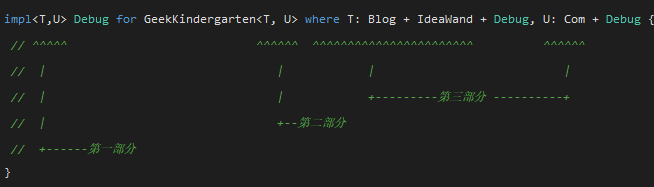
\includegraphics[width=\linewidth]{rust_impl_split.png}
  \caption{泛型类型的解析}
  \label{fig:rust_impl_split}
\end{figure}

基于以上的基础,现在,我们添加上对于泛型参数的支持:
\begin{code-block}{rust}
fn get_generics(st: &syn::DeriveInput) -> syn::Generics {
    let mut generics_params = st.generics.clone();
    for param in generics_params.params.iter_mut() {
        // 如果是泛型参数T,则要求T必须满足本身实现了Debug Trait
        if let syn::GenericParam::Type(t) = param {
            // 对类型的末尾追加内容,即将std::fmt::Debug格式化成语法树节点
            t.bounds.push(parse_quote!(std::fmt::Debug));
        }
    }
    generics_params
}
fn generate_debug_trait(st: &syn::DeriveInput) -> syn::Result<proc_macro2::TokenStream> {
    ...
    let generics = get_generics(&st);
    let (impl_block, generic_block, where_block) = generics.split_for_impl();
    let ret = quote! {
        impl #impl_block std::fmt::Debug for #struct_name_ident #generic_block #where_block {
            fn fmt(&self, ft: &mut std::fmt::Formatter) -> std::fmt::Result {
                #debug_body
            }
        }
    };

    Ok(ret)
}
\end{code-block}
其余的代码保持不变。接下来,使用示例代码进行测试:
\begin{code-block}{rust}
#[derive(CustomDebug)]
pub struct Custom {
    name: String,
    #[debug = "0b{:08b}"]
    age: u8,
}
\end{code-block}
这种没有泛型参数的,不会有什么变化,通过\codeinline{bash}{cargo expand}展开之后
的结果基本和之前是相同的;如果将代码进行修改,添加上泛型参数:
\begin{code-block}{rust}
#[derive(CustomDebug)]
pub struct Custom<T, U> {
    name: T,
    #[debug = "0b{:08b}"]
    age: U,
}
\end{code-block}
则展开之后的代码大致如下:
\begin{figure}[H]
  \centering
  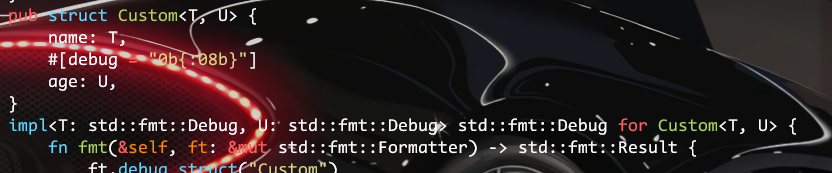
\includegraphics[width=\linewidth]{rust_with_generic.png}
  \caption{泛型参数的展开}
  \label{fig:rust_with_generic}
\end{figure}
而如果结构体当中包含了生命周期:
\begin{code-block}{rust}
#[derive(CustomDebug)]
pub struct Custom<'a, T> {
    name: &'a str,
    #[debug = "0b{:08b}"]
    age: u8,
    other: T,
}
\end{code-block}
则展开之后的结果大致如下:
\begin{figure}[H]
  \centering
  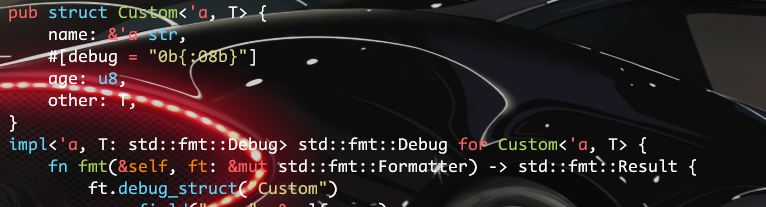
\includegraphics[width=\linewidth]{rust_with_generic_and_lifetime.png}
  \caption{泛型参数和生命周期的展开}
  \label{fig:rust_with_generic_and_lifetime}
\end{figure}

在上面的处理当中,泛型参数默认都是普通类型,并且没有进行嵌套。考虑下面的情况:
\begin{code-block}{rust}
pub struct GeekKindergarten<T, U> {
    blog: Foo<U>,
    ideawand: PhantomData<T>,
}
\end{code-block}
如果按照之前的处理方式,那我们的过程宏对泛型参数的处理,生成的限定条件应该是
\codeinline{rust}{T: Debug, U: Debug}。但是,由于在Rust当中,\codeinline{rust}{PhantomData}
本身就已经实现了Debug Trait,因此,从实际上讲,是没有必要对U或者\codeinline{rust}{PhantomData<U>}做
Trait限定的。面对这类本身已经实现了Debug的泛型结构体,有一种应对办法,即在生成Trait限定时,
不是针对每一个泛型参数去限制,而是对结构体中每一个字段的类型来添加限制,简而言之,
限定条件应该修改为\codeinline{rust}{Foo<U>: Debug, PhantomData<T>: Debug}。
\begin{critical}
但是这种方式的副作用非常大,因此,在实际的生产环境当中,几乎无人使用。
\end{critical}

由于\codeinline{rust}{PhantomData}在Rust当中使用非常频繁,通常的做法是:判断是否
包含\codeinline{rust}{PhantomData}类型的字段,如果有,则查看被其包裹的泛型参数
是否只是在\codeinline{rust}{PhantomData}当中出现过,如果是,则不对相关的泛型参数添加Debug Trait限定了。
以下面的代码为例:
\begin{code-block}{rust}
struct GeekKindergarten<T, U, V, W> {
    blog: T,
    ideawand: PhantomData<U>,
    com: U,
    foo: PhantomData<V>,
    bar: Baz<W>,
}
\end{code-block}

\begin{note}
\begin{enumerate}
  \item 泛型参数\codeinline{rust}{T}没有出现在\codeinline{rust}{PhantomData}的类型当中,因此,需要添加Debug Trait限定
  \item 泛型参数\codeinline{rust}{U}出现在了\codeinline{rust}{PhantomData}当中,但是,由于其同时作为了结构体的其他字段,因此,仍然需要添加Debug限定
  \item \codeinline{rust}{V}只出现在了\codeinline{rust}{PhantomData}当中,无需添加Debug限定
  \item \codeinline{rust}{W}虽然被其他的类型包裹,但是并没有出现在\codeinline{rust}{PhantomData},因此,同样需要增加Debug限定
\end{enumerate}
\end{note}

根据这些提示,需要首先针对\codeinline{rust}{PhantomData}进行处理,即将其包裹的
数据类型提取出来,在处理之前,首先看看包含了\codeinline{rust}{PhantomData}的
结构体字段的语法树结构:
\begin{code-block}{rust}
#[derive(CustomDebug)]
pub struct Custom<'a, T, U> {
    name: &'a str,
    #[debug = "0b{:08b}"]
    age: u8,
    other: T,
    phd: PhantomData<U>,
}
\end{code-block}
以上述代码为例,其phd字段的语法树结构如下:
\begin{code-block}{json}
Field {
    attrs: [],
    vis: Inherited,
    ident: Some(
        Ident {
            ident: "phd",
            span: #0 bytes(2201..2204),
        },
    ),
    colon_token: Some(
        Colon,
    ),
    ty: Path(
        TypePath {
            qself: None,
            path: Path {
                leading_colon: None,
                segments: [
                    PathSegment {
                        ident: Ident {
                            ident: "PhantomData",
                            span: #0 bytes(2206..2217),
                        },
                        arguments: AngleBracketed(
                            AngleBracketedGenericArguments {
                                colon2_token: None,
                                lt_token: Lt,
                                args: [
                                    Type(
                                        Path(
                                            TypePath {
                                                qself: None,
                                                path: Path {
                                                    leading_colon: None,
                                                    segments: [
                                                        PathSegment {
                                                            ident: Ident {
                                                                ident: "U",
                                                                span: #0 bytes(2218..2219),
                                                            },
                                                            arguments: None,
                                                        },
                                                    ],
                                                },
                                            },
                                        ),
                                    ),
                                ],
                                gt_token: Gt,
                            },
                        ),
                    },
                ],
            },
        },
    ),
}
\end{code-block}
因此,提取\codeinline{rust}{PhantomData}字段的包裹数据类型操作大致如下:
\begin{code-block}{rust}
fn get_phantomdata_generic_type_name(
    filed: &syn::Field,
) -> syn::Result<Option<String>> {
    if let syn::Type::Path(syn::TypePath {
        path: syn::Path { ref segments, .. },
        ..
    }) = filed.ty {
        if let Some(syn::PathSegment {
            ref ident,
            ref arguments,
        }) = segments.last()
        {
            if ident == "PhantomData" {
                if let syn::PathArguments::AngleBracketed(
                    syn::AngleBracketedGenericArguments {
                        args, .. }) = arguments
                {
                    if let Some(syn::GenericArgument::Type(
                        syn::Type::Path(ref arg_path))) = args.first()
                    {
                        if let Some(generic_ident) =
                                arg_path.path.segments.first() {
                            return Ok(Some(generic_ident.ident.to_string()));
                        }
                    }
                }
            }
        }
    }
    Ok(None)
}
\end{code-block}
同样的,也需要将其他字段的类型提取出来,需要注意类似\codeinline{rust}{bar: Baz<W>}这种,
只需要将其中的Baz类型提取出来。这种字段的语法树结构和上面的类似,只是\codeinline{rust}{PhantomData}
被其他的数据类型所替换而已,因此,其处理函数非常类似:
\begin{code-block}{rust}
fn get_field_type_name(
    field: &syn::Field,
) -> syn::Result<Option<String>> {

    if let syn::Type::Path(
        syn::TypePath {
            path: syn::Path { ref segments, .. },
            ..
    }) = field.ty
    {
        if let Some(syn::PathSegment {
            ref ident, .. }) = segments.last() {
            return Ok(Some(ident.to_string()));
        }
    }
    Ok(None)
}
\end{code-block}

有了上述的基础之后,接下来修改其他函数:
\begin{code-block}{rust}
fn get_generics(
    st: &syn::DeriveInput,
) -> syn::Result<syn::Generics> {
    let fields = get_filed_from_derive_input_debug(st)?;
    let mut generics_params = st.generics.clone();
    let mut field_type_name = Vec::new();
    let mut phantomdata_type_param_names = Vec::new();

    for field in fields {
        if let Some(name) = get_field_type_name(&field)? {
            field_type_name.push(name);
        }
        if let Some(phd) = get_phantomdata_generic_type_name(&field)? {
            phantomdata_type_param_names.push(phd);
        }
    }

    for param in generics_params.params.iter_mut() {
        if let syn::GenericParam::Type(t) = param {
            let type_name = t.ident.to_string();
            // 如果PhantomData类型包裹了对应的类型,
            // 并且,结构体的原始字段并不包含对应的类型
            // 则不追加Debug限定
            if phantomdata_type_param_names.contains(&type_name)
                && !field_type_name.contains(&type_name)
            {
                continue;
            }
            t.bounds.push(parse_quote!(std::fmt::Debug));
        }
    }
    Ok(generics_params)
}
\end{code-block}

然后对示例代码进行展开:
\begin{code-block}{rust}
#[derive(CustomDebug)]
pub struct Custom<'a, T, U, W, X> {
    name: &'a str,

    #[debug = "0b{:08b}"]
    age: u8,
    other: T,
    phd: PhantomData<U>,
    www: Bar<W>,
    phd2: PhantomData<X>,
    xxx: X,
}
\end{code-block}
则得到的结果如下:
\begin{figure}[H]
  \centering
  
\includegraphics[width=\linewidth]{rust_with_generic_and_phantomdata.png}
  \caption{包含嵌套泛型参数的CustomDebug}
  \label{fig:rust_with_generic_and_phantomdata}
\end{figure}
可以看到,展开的结果完全符合之前的需求和条件。

\subsection{过程宏案例-深度嵌套泛型与Visitor模式}
Trait在Rust当中使用非常广泛,也经常用于泛型嵌套当中。比如,\colorblock{Rust当中的关联类型},就
经常和Trait以及泛型结合在一起:
\begin{code-block}{rust}
trait Contains {
    type A; // Trait Contains的关联类型
    type B; // Trait Contains的关联类型
    fn contains(&self, _: &Self::A, _: &Self::B) -> bool;
    fn first(&self) -> Self::A;
    fn last(&self) -> Self::B;
}

struct Container(i32, i32);

impl Contains for Container {
    // 指出 `A` 和 `B` 是什么类型。如果 `input`(输入)类型
    // 为 `Container(i32, i32)`,那么 `output`(输出)类型
    // 会被确定为 `i32` 和 `i32`。
    type A = i32;
    type B = i32;

    fn contains(&self, number_1: &Self::A, number_2: &Self::B) -> bool {
        (&self.0 == number_1) && (&self.1 == number_2)
    }

    fn first(&self) -> Self::A { self.0 }

    fn last(&self) -> Self::B { self.1 }
}
\end{code-block}

假设有下面的代码:
\begin{code-block}{rust}
pub trait Trait {
    type Value;
}

pub struct Geek<T:Trait> {
    blog: T::Value,
    ideawand: PhantomData<T::Value>,
    com: Foo<Bar<Baz<T::Value>>>,
}
\end{code-block}
如果我们需要对上述的结构体\codeinline{rust}{Geek}进行语法树节点的解析,比如,针对
\codeinline{rust}{com: Foo<Bar<Baz<T::Value>>>}当中的\codeinline{rust}{T::Value}
进行解析和提取,就比较麻烦,按照之前的介绍,则需要使用很多层的\codeinline{rust}{if-let}
进行解构。比较幸运的是,\codeinline{rust}{syn}提供了一种\colorblock{Visit访问模式}。

Visitor模式的核心原理在于定义了一个名为Visit的Trait,这个Trait包含了上百个类型的语法树
节点各自所对应的回调函数,当其遍历语法树时,每遍历到一个节点,就会调用相关的回调函数。
比如上面的需求,只需要筛选出\codeinline{rust}{syn::TypePath}类型的节点,所以只需要
实现这个节点所对应的回调函数即可,如果需要实现对其他类型的visit访问,则需要参考syn的
官方文档\footnote{\url{https://docs.rs/syn/1.0.64/syn/visit/index.html}}:
\begin{code-block}{rust}
use syn::visit::{self, Visit};

struct TypePathVisitor {
    generic_type_names: Vec<String>,
    associated_types: HashMap<String, Vec<syn::TypePath>>,
}

// 使用该结构体实现Visit Trait
impl<'ast> Visit<'ast> for TypePathVisitor {
    // 只实现对TypePath的访问回调
    fn visit_type_path(&mut self, node: &'ast syn::TypePath) {
        // 该示例当中,专门针对 T::Value这种类型的节点
        if node.path.segments.len() >= 2 {
            let generic_type_name = node.path.segments[0].ident.to_string();
            if self.generic_type_names.contains(&generic_type_name) {
                self.associated_types.entry(
                    generic_type_name).or_insert(
                        Vec::new()).push(node.clone());
            }
        }

        // 进行递归式的访问,否则,无法遍历所有满足条件的语法树节点
        visit::visit_type_path(self, node);
    }
}
\end{code-block}
然后对其他的结构体语法树进行visit模式的访问:
\begin{code-block}{rust}
fn get_generic_associated_types(
    st: &syn::DeriveInput,
) -> HashMap<String, Vec<syn::TypePath>> {
    let origin_generic_param_names: Vec<String> =
        st.generics.params.iter().filter_map(|f| {
            if let syn::GenericParam::Type(ty) = f {
                return Some(ty.ident.to_string());
            }

            return None;
        }).collect();

    // 构造visit模式的访问器
    let mut visitor = TypePathVisitor {
        generic_type_names: origin_generic_param_names,
        associated_types: HashMap::new(),
    };

    // 对语法树节点进行遍历访问
    visitor.visit_derive_input(st);

    return visitor.associated_types;
}
\end{code-block}
针对下列的代码:
\begin{code-block}{rust}
trait TraitA {
    type Value;
}

#[derive(CustomDebug)]
pub struct Custom<'a, T, U: TraitA> {
    name: &'a str,
    other: T,
    complex: PhantomData<U::Value>,
}
\end{code-block}
Visitor访问模式得到的结果大致如下:
\begin{figure}[H]
  \centering
  
\includegraphics[width=\linewidth]{rust_syn_visitor.png}
  \caption{Visitor模式访问语法树结构}
  \label{fig:rust_syn_visitor}
\end{figure}

有了上述的基础,可以对原有的代码进行修改了:针对关联数据类型,就不要对泛型参数T本身再添加约束了,
同时,关联类型的约束要放到where子句当中:
\begin{code-block}{rust}
fn get_generics(st: &syn::DeriveInput) -> syn::Result<syn::Generics> {
    ...
    let associated_types_map = get_generic_associated_types(st);
    for param in generics_params.params.iter_mut() {
        if let syn::GenericParam::Type(t) = param {
            let type_name = t.ident.to_string();
            if phantomdata_type_param_names.contains(&type_name)
                && !field_type_name.contains(&type_name)
            {
                continue;
            }
            // 针对关联数据类型,不对泛型参数`T`本身再添加约束了
            // 除非`T`本身也被直接使用了
            if associated_types_map.contains_key(&type_name)
                && !field_type_name.contains(&type_name)
            {
                continue;
            }
            t.bounds.push(parse_quote!(std::fmt::Debug));
        }
    }
    // 在where字句当中,增加对关联数据类型的约束
    generics_params.make_where_clause();
    for (_, associated_types) in associated_types_map {
        for associated_type in associated_types {
            generics_params.where_clause.as_mut().unwrap().predicates
                .push(parse_quote!(#associated_type:std::fmt::Debug));
        }
    }
    Ok(generics_params)
}
\end{code-block}

到此,针对如下的代码进行展开:
\begin{code-block}{rust}
trait TraitA { type Value; }
#[derive(CustomDebug)]
pub struct Custom<'a, T, U: TraitA> {
    name: &'a str,
    #[debug = "0b{:08b}"]
    age: u8,
    other: T,
    complex: PhantomData<U::Value>,
}
\end{code-block}
则展开之后的结果大致如下:
\begin{figure}[H]
  \centering
  
\includegraphics[width=\linewidth]{rust_associate_debug.png}
  \caption{包含关联数据类型的Debug展开}
  \label{fig:rust_associate_debug}
\end{figure}

\section{多线程}
Rust也同样支持常见的并行和并发操作,也同样分为进程,线程以及消息通信等等。

\subsection{线程}
Rust的线程操作必须使用闭包完成。在之前看到的闭包当中,通常采用的都是有参的闭包,
而在Rust的线程操作当中,则经常会遇到无参数的闭包;Rust的线程使用thread::spawn函数
进行实现:
\begin{code-block}{rust}
use std::thread;
use std::time::Duration;

fn main() {
    thread::spawn(|| {
        for i in 1..10 {
            println!("hi number {} from the spawned thread!", i);
            thread::sleep(Duration::from_millis(1));
        }
    });

    for i in 1..5 {
        println!("hi number {} from the main thread!", i);
        thread::sleep(Duration::from_millis(1));
    }

}
\end{code-block}
和其他语言的线程概念一样,当主线程结束时,所有的线程都会被终止。因此上述代码当中,
子线程(spawn)无法将所有的循环执行完成。为了达成所有进/线程执行完成之后才退出主
进/线程的目的,和其他的开发语言相同,需要在主进程当中调用join函数:
\begin{code-block}{rust}
fn main() {

    let handle = thread::spawn(|| {
        for i in 1..10 {
            println!("hi number {} from the spawned thread!", i);
            thread::sleep(Duration::from_millis(1));
        }
    });

    for i in 1..5 {
        println!("hi number {} from the main thread!", i);
        thread::sleep(Duration::from_millis(1));
    }

    handle.join().unwrap();
}
\end{code-block}
Thread::spawn的返回值是JoinHandle,是一个拥有所有权的值,当对其调用join方法时,
它会等待对应线程结束;而join的返回值是一个Result,可以按照之前介绍的方式进行处理。
同时,Join函数是一个阻塞式函数,只有当该函数运行结束之后,才会继续进行后续的操作。

多数情况下,Rust的线程不可能只会在内部运行,而和外部没有数据交互。但是,如果我们
直接使用外部数据,则会出现错误,比如下方的代码:
\begin{code-block}{rust}
fn main() {
    let v = vec![1, 2, 3];

    let handle = thread::spawn(|| {
        println!("Here's a vector: {:?}", v);
    });

    handle.join().unwrap();
}
\end{code-block}
\begin{figure}[H]
  \centering
  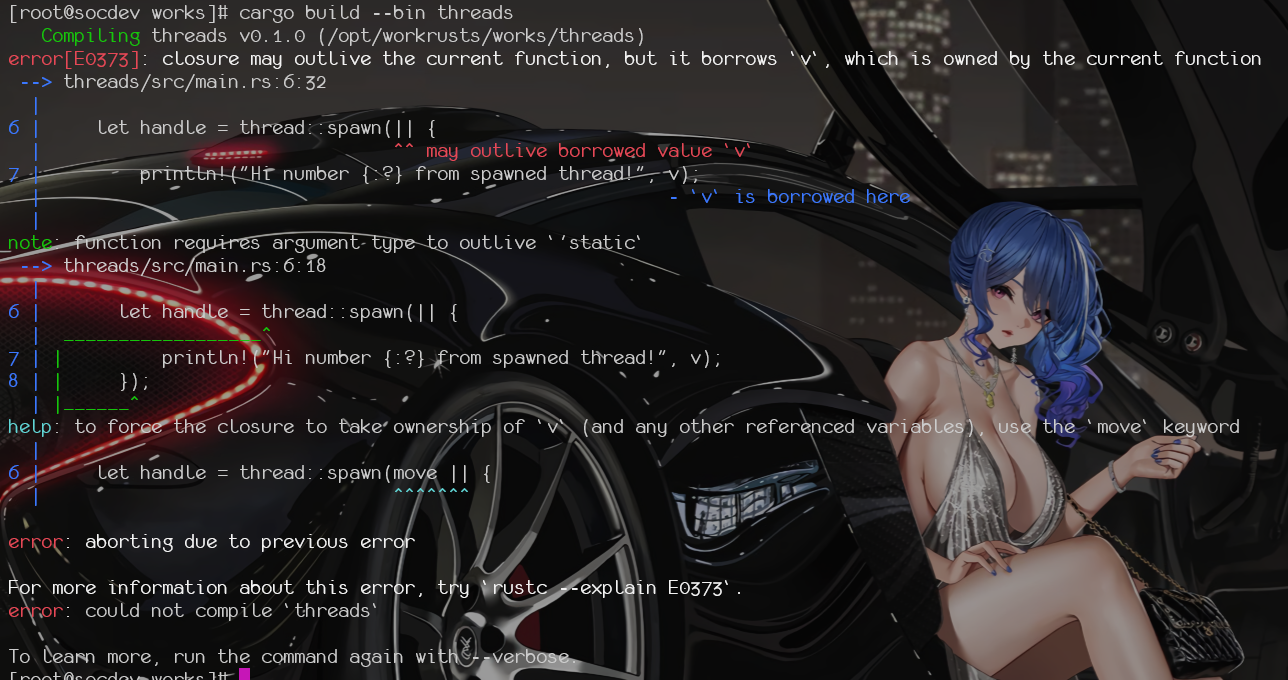
\includegraphics[width=\linewidth]{rust_thread_out_params.png}
  \caption{试图访问线程外部资源}
  \label{fig:rust_thread_out_params}
\end{figure}
线程使用的是闭包,从闭包的定义来说,是可以捕获并使用外部变量和数据的;但是,Rust
不知道这个线程到底会运行多长时间,因此无法知道对外部变量的引用是否一直有效,比如
下方的代码:
\begin{code-block}{rust}
fn main() {

    let v = vec![1, 2, 3];

    let handle = thread::spawn(|| {
        println!("Here's a vector: {:?}", v);
    });

    drop(v);

    handle.join().unwrap();
}
\end{code-block}
启动线程的同时,立即将v进行丢弃,线程内部无法知道v在运行阶段是否继续有效,就会
出现错误,因此,如果在线程当中使用默认的闭包模式,则无法对应的闭包是无法捕获以及
使用外部的变量和数据的。此时,则需要使用move闭包进行替换,即强制闭包获取外部变量
的所有权,而不是由Rust进行借用推断。但是需要注意,一旦使用move之后,在线程之外,
变量将无法再进行使用:
\begin{code-block}{rust}
fn main() {
    let v = vec![1, 2, 3];

    let handle = thread::spawn(move || {
        println!("Here's a vector: {:?}", v);
    });

    // 下方代码无法再进行执行
    // println!("{:?}", v);

    handle.join().unwrap();
}
\end{code-block}

\subsection{消息通信和消息传递}
每个线程做自己的事情,但是,不管什么编程语言,都需要考虑线程之间的数据交互问题。
Rust向Golang进行了学习,使用通信替换共享内存,来进行线程之间的数据传输。同样的,
Rust当中用于消息传递并发的主要工具是通道,该概念和Golang的通道概念相同。Rust的通道
分为2个角色:发送者和接收者,发送者发送消息,接收者接收消息,当发送者或者接收者任一
被丢弃时,则对应的通道被视为关闭。

Rust的通道采用mpsc::channel函数实现,mpsc表示多个生产者,单个消费者,因此,Rust
标准库实现通道的方式意味着一个通道可以有多个产生值的发送(sending)端,但只能有
一个消费这些值的接收(receiving)端。通道的实现示例如下:
\begin{code-block}{rust}
use std::sync::mpsc;

fn main() {
    let (sender, recevier) = mpsc::channel();
}
\end{code-block}
其中,函数的第一个返回值为发送者,第二个参数为接收者。使用通道发送数据通信的示例
如下:
\begin{code-block}{rust}
use std::sync::mpsc;
use std::thread;

fn main() {
    let (sender, recevier) = mpsc::channel();

    thread::spawn(move || {
        let val = "lucifer".to_string();

        match sender.send(val) {
            Ok(_) => println!("Send success"),
            Err(error) => println!("Send failed :{:?}", error),
        }

    });

    let res = match recevier.recv() {
        Ok(s) => s,
        Err(error) => {
            println!("Cannot recevie anything from sender: {:?}", error);
            "".to_string()
        }
    };

    println!("The result of channel is {}", res);
}
\end{code-block}
接收者接收消息有2种模式:默认的recv是阻塞式,返回一个Result<T, E>,当通道关闭时,
将返回Result当中的Error;而try\_recv是非阻塞式,同样是返回一个Result<T, E>,但是,
Result当中的Error表示没有接收到任何消息,可以使用for循环进行反复的尝试读取操作。
另外需要注意的是,Send函数会改变变量的所有权,当该函数执行之后,被发送的消息
(变量)将无法再使用。

但是,通道可以反复使用,而且和Golang的类似,Rust的通道也是可以进行迭代的,特别
是在接收消息时,通常采用for循环进行操作,减少了错误处理的代码,使得代码更具可读性:
\begin{code-block}{rust}
use std::sync::mpsc;
use std::thread;

fn main() {
    let (sender, recevier) = mpsc::channel();

    let handler = thread::spawn(move || {

        let vals = vec!["lucifer", "titans", "garuda"];

        for val in vals {
            match sender.send(val) {
                Ok(_) => println!("Send success"),
                Err(error) => println!("Send failed :{:?}", error),
            }
        }

    });

    for msg in recevier {
        println!("The msg is {}", msg);
    }

    match handler.join() {
        Err(error) => println!("Error{:?}", error),
        _ => (),
    }
}
\end{code-block}

同样的,由于Rust的通道默认是多生产者/单消费者,因此,可以通过多个发送端向单个接
收端发送消息。实际使用当中的多个发送端,则通常是某个发送端的克隆对象,如下:
\begin{code-block}{rust}
use std::sync::mpsc;
use std::thread;

fn main() {
    let (sender, recevier) = mpsc::channel();
    let sender_copy = sender.clone();

    let handler = thread::spawn(move || {
        let vals = vec!["lucifer", "titans", "garuda"];

        for val in vals {
            match sender.send(val) {
                Ok(_) => println!("Send success"),
                Err(error) => println!("Send failed :{:?}", error),
            }
        }
    });

    let handler_copy = thread::spawn(move || {
        let vals = vec!["zhangjl", "luoyan", "zhangzz"];

        for val in vals {
            match sender_copy.send(val) {
                Err(error) => println!("Send failed :{:?}", error),
                _ => (),
            }
        }
    });

    for msg in recevier {
        println!("The msg is {}", msg);
    }

    match handler_copy.join() {
        Err(error) => println!("Error{:?}", error),
        _ => (),
    }

    match handler.join() {
        Err(error) => println!("Error{:?}", error),
        _ => (),
    }
}
\end{code-block}

\subsection{共享状态}
在其他语言当中,有些特殊的场景,还是必须使用原有的线程并发概念——锁——来进行资源的
访问/读写控制。Rust当中同样存在锁,比较常见的就是互斥锁(互斥器,Mutex)以及原子
计数器(Arc)。在基本的操作上,互斥锁的使用和其他语言当中没有太大的区别:
\begin{code-block}{rust}
use std::sync::Mutex;

fn main() {

    let m = Mutex::new(5);
    {
        let mut num = m.lock().unwrap();
        *num = 6;
    }

    println!("m = {:?}", m);
}
\end{code-block}
注意,上述代码如果将内部大括号去除,则运行结束之后,m的状态还是锁定状态;但是,
有大括号,则表示大括号内部的段是一个有效的生命周期,当该生命周期结束之后,互斥
锁将自动释放。一旦获取了锁,就可以将返回值(在这里是num)视为一个其内部数据的
\colorblock{可变引用}。类型系统确保了我们在使用m中的值之前
获取锁:Mutex<i32>并不是一个i32,所以必须获取锁才能使用这个i32值。

实质上,Mutex是一个智能指针,lock调用返回一个叫做MutexGuard的智能指针。这个智能
指针实现了Deref来指向其内部数据;同时也提供了一个Drop实现,使得MutexGuard离开作
用域时自动释放锁,即锁的释放是自动发生的。

但是默认情况下,Mutex是无法用于进行线程间的数据共享,如下:
\begin{code-block}{rust}
use std::rc::Rc;
use std::sync::Mutex;
use std::thread;

fn main() {
    let counter = Rc::new(Mutex::new(0));
    let mut handles = vec![];

    for _ in 0..10 {
        let counter = Rc::clone(&counter);
        let handle = thread::spawn(move || {
            let mut num = counter.lock().unwrap();
            *num += 1;
        });

        handles.push(handle);
    }

    for handle in handles {
        handle.join().unwrap();
    }

    println!("Result: {}", *counter.lock().unwrap());
}
\end{code-block}
上述代码会出现下面的类似错误:
\begin{figure}[H]
  \centering
  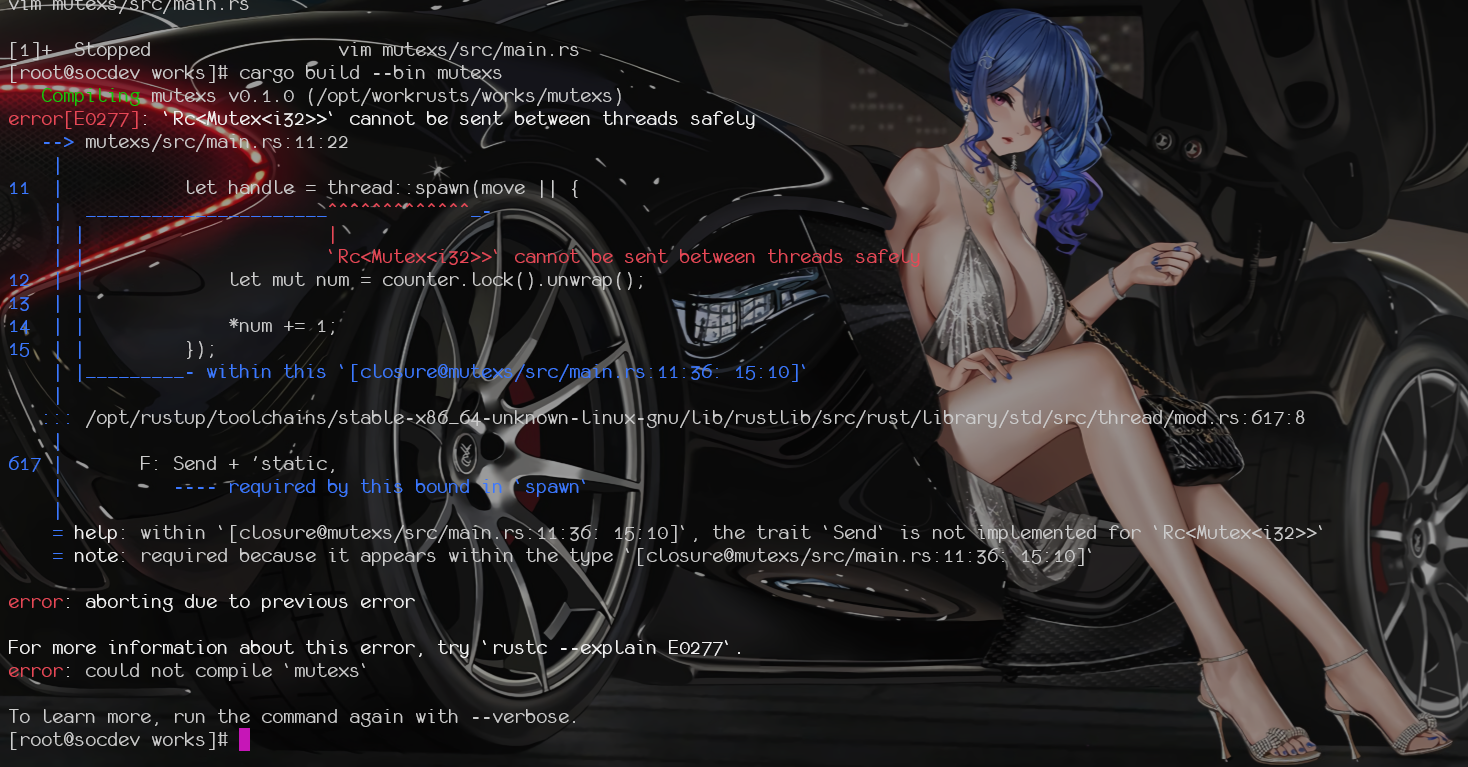
\includegraphics[width=\linewidth]{rust_mutex_share_error.png}
  \caption{试图通过Rc共享Mutex的数据}
  \label{fig:rust_mutex_share_error}
\end{figure}
即之前提到的,Rc类型只能用于单线程/单进程环境。

而共享引用计数则需要使用Arc,它是可以安全的用于并发环境的类型,即原子引用计数,
可以在线程间进行共享所有权。Arc和Rc有相同的API,基本使用方法上类似。所有,可以直
接对上述代码进行修改:
\begin{code-block}{rust}
use std::sync::{Arc, Mutex};
use std::thread;

fn main() {
    let counter = Arc::new(Mutex::new(0));
    let mut handles = vec![];

    for _ in 0..10 {
        let counter = Arc::clone(&counter);
        let handle = thread::spawn(move || {
            let mut num = counter.lock().unwrap();
            *num += 1;
        });

        handles.push(handle);
    }

    for handle in handles {
        handle.join().unwrap();
    }

    println!("Result: {}", *counter.lock().unwrap());
}
\end{code-block}
通过这样简单的修改,成功实现了10个进程当中对同一个数值进行加法操作的功能。

虽然Rust本身的线程/进程管理非常完善,但是,thread::spawn产生的线程没有名称,并且
其栈空间大小默认为2M,如果需要需要针对线程/进程进行粒度更细的操作,比如自定义
线程名称,自定义线程的资源等等,此时,就需要使用thread::Builder进行修改,具体示例
如下:
\begin{code-block}{rust}
let mut v_thread = vec![];

for id in 1..5 {
    let thread_name = format!("child-{}", id);
    let size: usize = 1024;

    // 定义线程的名称,设置线程占用的栈大小为1M(1024)
    let builder = Builder::new().name(thread_name).stack_size(size);

    // builder.spawn返回的是Result<JoinHander, std::io::Error>
    // 需要进行处理,取出真正的线程句柄
    match builder.spawn(move || {
        info!(
            "In the child: {}, and the child name is {}",
            id,
            current().name().unwrap()
        );
    }) {
        Ok(child) => v_thread.push(child),
        Err(error) => error!(
            "Cannot create the thread {} because: {:?}", id, error),
    };
}

// 其他的同普通的线程,
for child in v_thread {
    child.join().unwrap();
}

\end{code-block}

由于线程包含自己的资源空间,因此,存在一个特殊的存储空间——线程本地存储(Thread Local Storage,TLS),
存放在该区域的资源,其他线程无法访问,而是每个线程独占的数据:
\begin{code-block}{rust}
use std::cell::RefCell;
use std::thread;

fn main() {
    // 在线程本地存储定义一个FOO变量,最终的类型是thread::LocalKey
    thread_local!(static FOO: RefCell<u32> = RefCell::new(1));

    // 提供了一个with方法,可以通过给该方法传入闭包
    // 来操作线程本地存储中包含的变量
    FOO.with(|f| {
        info!("The f borrow is {}", *f.borrow());
        *f.borrow_mut() = 2;
    });

    let handler = thread::spawn(move || {

        // 子线程也有一个线程本地存储实例FOO,为主线程的副本
        // 也可以使用thread_local!宏在该子线程中重新创建一个LocalKey实例
        FOO.with(|f| {
            info!("In the handler thread The f borrow is {}", *f.borrow());
            *f.borrow_mut() = 3;
        });
    });

    // 主线程当中FOO实例并没有被子线程修改为3
    // thread local!宏定义单个线程内的一些独享数据
    FOO.with(|f| {
        info!("The f borrow is {}", *f.borrow());
    });

    handler.join().unwrap();
}
\end{code-block}

在同步原语支持方面,Rust也有自己的实现方式,通过使用std::thread当中的park函数提供
阻塞线程的能力,但并不能永久的阻塞线程,存在时间限制;而\codeinline{rust}{std::thread::part_timeout}
则可以显式的指定阻塞的超时时间;std::thread::Thread::unpark则可以将阻塞的线程重启;
如果需要让出当前线程的时间片,则需要使用std::thread::yeild\_now,让其他线程进行执行。
简单的阻塞例子如下:
\begin{code-block}{rust}
use std::thread::{self, Builder};
use std::time::Duration;

fn main() {
    let parked_thread = Builder::new()
        .spawn(|| {
            info!("Parking the thread ...");
            // 阻塞当前线程
            thread::park();
            info!("Thread parked");
        })
        .unwrap();

    thread::sleep(Duration::from_secs(5));

    info!("Unparking the thread");

    // 从JoinHandle中得到具体的线程
    parked_thread.thread().unpark();

    // 将该线程重新启动,该线程会继续沿着之前暂停的上下文执行
    parked_thread.join().unwrap();
}
\end{code-block}

除了常见的互斥锁(Mutex)之外,Rust也支持读写锁(RwLock)。读写锁的基本示例如下:
\begin{code-block}{rust}
use std::sync::RwLock;

fn main() {
    let rw_lock = RwLock::new(5);

    // 读写锁的使用必须使用{}进行区分,即便是单独使用读或者写也是一样
    // 通过代码块{},让读写锁自动释放,否则会出现死锁
    {
        let read_1 = rw_lock.read().unwrap();
        let read_2 = rw_lock.read().unwrap();
        info!("The read_1 is {}, and read_2 is {}", read_1, read_2);
    }

    {
        let mut write = rw_lock.write().unwrap();
        *write = 100;
    }

    info!("The data is {:?}", rw_lock);
}
\end{code-block}

而针对于同步的需求,Rust提供了屏障(Barrier)和条件变量(Condition Variable)原语。
屏障,是要求所有的条件全部满足之后,再进行后续操作,即在满足某个条件前,阻塞全部的
线程,通常用于线程同步,如下:
\begin{code-block}{rust}
use std::sync::{Arc, Barrier};
use std::thread;

fn main() {
    let mut vec = vec![];

    let barrier = Arc::new(Barrier::new(5));

    for id in 0..5 {
        let barrier_copy = barrier.clone();
        vec.push(thread::spawn(move || {
            info!("Thread {} Waiting the other threads...", id);
            // wait阻塞了所有的线程,当所有线程的wait之前部分全部执行完成之后
            // wait操作才算执行完成,才会执行每个线程后续的操作
            barrier_copy.wait();

            info!("{} After wait...", id);
        }));
    }
    for handler in vec {
        handler.join().unwrap();
    }
}
\end{code-block}

而条件变量与屏障稍微的区别在于,它不是阻塞所有的线程,而是在满足特定条件前,阻塞
一个得到了互斥锁的线程,如下:
\begin{code-block}{rust}
use std::sync::{Arc, Condvar, Mutex};
use std::thread;
use std::time::Duration;
fn main() {
    // 生成包含互斥锁的条件变量condvar
    let pair = Arc::new(((Mutex::new(false)), Condvar::new()));
    let pair_clone = pair.clone();
    let handler = thread::spawn(move || {
        let &(ref lock, ref cvar) = &*pair_clone;
        // 获得互斥锁
        let mut started = lock.lock().unwrap();
        info!("In the child thread");
        thread::sleep(Duration::from_secs(5));
        *started = true;
        // 通知主线程
        cvar.notify_one();
    });
    let &(ref lock, ref cvar) = &*pair;
    let mut started = lock.lock().unwrap();
    while !*started {
        info!("Waiting for the started singal {} ...", started);
        // 使用条件变量的wait阻塞当前线程,一直到cvar退出
        started = cvar.wait(started).unwrap();
        info!("Started singal finished {} ...", started);
    }
    handler.join().unwrap();
}
\end{code-block}
相比于单纯的互斥锁必须多次出入临界区才能获取到某个状态的信息,条件变量减少了系统
资源的浪费,但是需要注意,每个条件变量每次只能和一个互斥锁(体)一起使用。

除了使用锁、屏障以及条件变量,关于同步的问题,还可以使用原子操作。Rust目前只提供了
4个原子操作类型:AtomicBool、Atomiclsize、AtomicPtr和AtomicUsize。需要注意,虽然原子
操作类型本身可以保证操作的原子性,但是其本身并没有提供跨线程的共享方法,如果需要
使得原子数据类型也可以在线程间共享,则应当使用Arc进行封装,比如下面,使用原子类型
实现一个自旋锁:
\begin{code-block}{rust}
use std::sync::atomic::{AtomicUsize, Ordering};
use std::sync::Arc;
fn main() {
    let spinlock = Arc::new(AtomicUsize::new(1));
    let spinlock_clone = spinlock.clone();
    let handler = thread::spawn(move || {
        // 将原子类型的数据设置为0
        spinlock_clone.store(0, Ordering::SeqCst);
    });
    // 使用spinlock的load方法读取其内部原子类型的值,如果不为0,
    // 则不停地循环测试锁的状态,直到其状态被置为0为止
    // 所谓“自旋”就是指在语义上表示这种不断循环获取锁状态的行为
    while spinlock.load(Ordering::SeqCst) != 0 {}
    handler.join().unwrap();
}
\end{code-block}
代码当中的Ordering表示内存参数顺序,可以通过该参数来控制底层线程执行顺序。默认的,
Rust支持5种内存顺序,归为3大类:
\begin{itemize}
  \item 排序一致性顺序——SeqCst:最简单直观,要求必须先存储,后读取,在多线程环境下,所有的原子写操作都必须在读操作之前完成,强行指定了线程的执行顺序,保证了多线程中所有操作的全局一致性,但是存在性能损耗,其实质类似于餐厅点餐,相当于强制要求所有需要结账的客人,必须等所有点单的客户完成之后才可以结账
  \item 自由顺序——Relaxed:和SeqCst相反,完全不会对线程的顺序进行干涉,线程只进行原子操作,但是,线程之间会存在竞态条件,使用这种内存顺序会比较危险,只有在明确了解当前使用场景且必须使用它的情况下(比如只有读操作),才可使用自由顺序
  \item 获取-释放顺序——Release,Acquire和AcqRel: 是除排序一致性顺序之外的优先选择,默认情况下,不会对全部线程进行统一强制性的执行顺序要求,store表示释放(release),而load表示获取(acquire),通过这2种操作的协作实现线程同步。Release表示使用该顺序的store操作,之前所有的操作对于使用Acquire顺序的load操作都可见;反之,使用使用Aquire顺序的load操作,对于使用Release的store操作都是可见的;AcqRel表示读时使用Acquire顺序的load操作,写时使用Release顺序的store操作。获取释放顺序虽然不像排序一致性顺序那样对全局线程统一排序,但是它让每个线程都能接固定的顺序执行。
\end{itemize}

在此之前,已经谈到Rust支持channel通信来解决多线程环境所遇到的问题,比如之前的小例子:
\begin{code-block}{rust}
use std::thread;
use std::sync::mpsc::channel;
fn main() {
    let (tx, rx) = channel();
    let handler = thread::spawn(move || {
        tx.send(10).unwrap();
    });
    let res = rx.recv().unwrap();
    handler.join().unwrap();
}
\end{code-block}
像这种只有2个线程间通信的channel,称之为流通道,在流通道的内部,默认使用的是单生产者
单消费者的模式来提升性能。在此之前,我们看到多个发送者(生产者)单个接收者(消费者)
模式的通道,则称之为共享通道。而由于统一使用的channel函数生成通道,这样的通道又
称之为异步通道,即所有的操作都可以异步的进行处理,不会出现线程阻塞的情况。

同步通道的例子则如下:
\begin{code-block}{rust}
use std::thread;
use std::sync::mpsc::sync_channel;
fn main() {
    // 创建缓冲区为1的同步通道
    let (tx, rx) = sync_channel(1);
    tx.send(1).unwrap();
    let handler = thread::spawn(move || {
        tx.send(2).unwrap();
    });
    let res1 = rx.recv().unwrap();
    info!("The result is {}", res1);
    let res2 = rx.recv().unwrap();
    info!("The result2 is {}", res2);
    handler.join().unwrap();
}
\end{code-block}
在上述代码当中,由于channel的缓冲区设置为1,所以,当第一条信息被消费(recv)之前,
后续的消息发送会被一直阻塞,直到缓冲区可用为止。

虽然channel解决了很多的多线程同步和共享问题,但是,channel并没有解决死锁的问题,
当设计不周到的时候,channel同样会出现死锁的问题:
\begin{code-block}{rust}
use std::thread;
use std::sync::mpsc::channel;
fn main() {
    let (tx, rx) = channel();
    let mut handlers = vec![];
    for i in 0..5 {
        let tc = tx.clone();
        let handler = thread::spawn(move || {
            tc.send(i).unwrap();
        });
        handlers.push(handler);
    }
    // 如果注释下面代码,主线程将一直不退出
    // drop(tx);
    for j in rx.iter() {
        info!("{:?}", j);
    }
    for handler in handlers {
        handler.join().unwrap();
    }
}
\end{code-block}
因为rx的iter方法会阻塞线程,只要tx还没有被析构,该迭代器就会一直等待新的消息,
只有tx被析构之后,迭代器才能返回None,从而结束退出main主线程。由于上述代码的tx
一直没有析构,所以迭代器依旧会进行等待,但是tx也没有发送信息,从而造成死锁的状态。
显式调用drop之后,死锁将不会存在。

\section{异步编程(Future)的基本原理}
Rust目前的版本当中,异步/同步的支持比较完善,通常需要使用Future进行实现,
其中futures\footnote{\url{https://github.com/rust-lang/futures-rs}}提供了一个比较基本的异步编程实现,
Tokio\footnote{\url{https://github.com/tokio-rs/tokio}}也提供了比较完整的平台支持,
Async-Std\footnote{\url{https://github.com/async-rs/async-std}}也提供了
相关的支持。多线程的劣势主要体现在操作系统调度开销,难度较大,线程切换以及
跨线程共享数据会产生很多的额外开销,这些就是异步并发(async/await)发挥作用的
重要场景。

\subsection{Future的基本原理与实现机制}
所谓的Futrue,从字面上讲,就是一些将来完成的操作,也就是一些并不是当前立即结束
的操作,以此指代Rust的异步操作。Rust的异步操作实现基于轮询机制,每个异步任务分成
了3个阶段:
\begin{enumerate}
  \item 轮询阶段(Poll):一个Future被轮询之后,会开始执行,直到被阻塞。轮询Future通常被称为执行器(executor)
  \item 等待阶段:事件源(即需要使用Future的对象,通常称为reactor)注册等待事件发生,并确保当对应的事件发生或准备好时唤醒对应的Future
  \item 唤醒阶段:事件发生,相应的Future被唤醒,执行器执行,直至完成
\end{enumerate}

例如对大文件进行操作,如果采用普通的文件打开方式,操作大文件,需要将文件内容打开
(全部在内存展开)之后,才能操作;而异步的文件打开,则相当于将文件句柄返回给调用
者,而后续的内容,在调用者需要进行使用时,再加载到内存当中。两者的具体的情况如下
所示:
\begin{figure}[H]
  \centering
  % 禁止svg当中的特殊文字转换
  \includesvg[inkscapelatex=false, width=\linewidth]{rust_async}
  \caption{同步与异步执行的区别\protect\footnotemark}
  \label{fig:rust_async}
\end{figure}
\footnotetext{同/异步:\url{https://os.phil-opp.com/async-await/async-example.svg}}
上述例子当中,轮询阶段就相当于询问文件是否被打开,而等待阶段,则相当于等待文件的
内容加载内存当中,唤醒,则是调用者访问文件内容。

Rust的异步实现依赖于Future。在标准库当中,Rust提供了Future的
Trait以及\codeinline{rust}{async}和\codeinline{rust}{await}2个异步并发的关键字,
但是并没有提供具体的实现(即运行时),运行时则是由其他的库提供的,常见的就包括
上面提到的Async-Std和Tokio,以及Rust官方提供的futures(不在Rust的标准库当中)。
Rust的异步运行时可以分为2部分:执行器(executor)和反应器(reactor),
这2部分则是由Waker(唤醒器)进行交互。

以futures为例,一个简单的异步应用大致如下:
\begin{code-block}{rust}
extern crate futures;
async fn foo() -> u8 { 8 }
async fn hello() {
    let res = foo().await;
    println!("The res is {}", res);
}

fn main() {
    let future = hello();
    futures::executor::block_on(future);
}
\end{code-block}
在上述的例子当中,使用关键字\codeinline{rust}{async}修饰的函数都是异步函数,这些
函数都会返回一个Future Trait,如果不使用\codeinline{rust}{async}关键字,实际上
也是可以实现异步函数的定义的,只不过,会相对比较麻烦,并且需要显式的使用Future,
比如下面的代码:
\begin{code-block}{rust}
use futures::future::{self, Future};
fn async_read_file(name: &str) -> impl Future<Output = String> {
    future::ready(String::from(name))
}
fn async_with_lifetime<'a>(input: &'a u8) -> impl Future<Output = u8> + 'a {
    future::ready(*input)
}
\end{code-block}

Rust的Future Trait的定义如下\footnote{定义:\url{https://doc.rust-lang.org/std/future/trait.Future.html}}:
\begin{code-block}{rust}
pub trait Future {
    type Output;
    fn poll(self: Pin<&mut Self>, cx: &mut Context) -> Poll<Self::Output>;
}
\end{code-block}
其中,Output指的是异步函数的返回数据类型,而\codeinline{rust}{poll}函数则是整个
Future工作机制的核心。该函数的实质是一个有限状态机,返回的Poll实际上是状态的描述。
Poll的定义如下:
\begin{code-block}{rust}
pub enum Poll<T> {
    Ready(T),
    Pending,
}
\end{code-block}
当异步函数的执行结果完成并且可用时,\codeinline{rust}{poll}函数将返回一个Ready
包裹的结果,表示完成;如果执行还没有结束,则会返回一个Pending,表示执行还将继续,
相关的数据还没有准备完成,需要继续等待或者轮询,并且从当前的context当中,克隆一个
waker,一旦future状态有新的变化,waker函数将被唤醒。注意,如果状态不是Ready,poll函数
会被再次调用(间隔一定时间),直到返回Ready之后,poll函数将不再被调用。如果用普通的
Rust代码进行表示,其内在的逻辑可以模拟如下(但是性能非常差):
\begin{code-block}{rust}
let future = async_read_file("foo.txt");
let file_content = loop {
    match future.poll(…) {
        Poll::Ready(value) => break value,
        Poll::Pending => {}, // do something
    }
}
\end{code-block}

而另一种思路,则是使用future的组合,比如下方的例子:
\begin{code-block}{rust}
use std::future::{self,Future};
use std::task::{Context, Poll};
use std::pin::Pin;
fn main() {
    let _ = file_len();
}
struct StringLen<F> {
    inner_future: F,
}
impl<F> Future for StringLen<F> where F: Future<Output = String>{
    type Output = usize;
    fn poll(mut self: Pin<&mut Self>, cx: &mut Context<'_>) -> Poll<Self::Output> {
        match self.inner_future.poll(cx) {
            Poll::Ready(s) => Poll::Ready(s.len()),
            Poll::Pending => Poll::Pending,
        }
    }
}
fn string_len(string: impl Future<Output = String>)
    -> impl Future<Output = usize>
{
    StringLen {
        inner_future: string,
    }
}
fn file_len() -> impl Future<Output = usize> {
    let file_content_future = async_read_file("foo.txt");
    string_len(file_content_future)
}
fn async_read_file(name: &str) -> impl Future<Output = String> {
    future::ready(String::from(name))
}
\end{code-block}
\begin{attention}
上述代码只是演示了一种Future可能的处理方式,但是,代码本身不可使用,原因在于在
上述代码当中还没有处理pin(固定)。
\end{attention}

通过future的组合,可以实现非常高效的代码,但是,在某些情况下,由于Rust的类型系统
以及基于闭包的接口,会使得future的组合使用起来比较难,比如下面的代码:
\begin{code-block}{rust}
use futures::future::{self, Either, Future, FutureExt};
fn main() {
    let _ = example(100);
}
fn example(min_len: usize) -> impl Future<Output = String> {
    async_read_file("foo.txt").then(move |content| {
        if content.len() < min_len {
            Either::Left(async_read_file("bar.txt").map(|s| content + &s))
        } else {
            Either::Right(future::ready(content))
        }
    })
}
fn async_read_file(name: &str) -> impl Future<Output = String> {
    future::ready(String::from(name))
}
\end{code-block}
上述代码的功能很简单,读取foo.txt文件,然后使用\codeinline{rust}{then}连接第二个
future:如果foo.txt的内容长度小于给定的最小值,则读取另一个文件bar.txt的内容,并将
其长度追加到返回结果当中,否则,只返回foo.txt的内容。上述操作当中,必须使用\codeinline{rust}{move}
关键字,否则会存在一个生命周期的错误;另外,if/else必须返回相同的类型,但是,
上述代码当中,if返回的是\codeinline{rust}{futures::future::Map},而else返回的是\codeinline{rust}{futures::future::Ready},
必须使用\codeinline{rust}{Either}将结果进行封装,转换成所期望的future。

\subsection{Future的async/await模式}
从上面的各种例子都可以看到,使用普通的方式实现Rust的异步编程可能会涉及到非常复杂的
代码,于是,Rust官方使用\codeinline{rust}{async/await}等关键字,来简化异步编程的实现,
屏蔽了繁琐的实现细节。使用上述两个关键字之后,Rust的编译器会在编译过程当中进行
自动转换,转换成Future的模式,比如:
\begin{code-block}{rust}
async fn foo() -> u32 {
    0
}
// 编译器内部会自动转换成这种模式
fn foo() -> impl Future<Output = u32> {
    future::ready(0)
}
\end{code-block}

但是,这个转换过程对于开发者而言是透明无感的,以上面代码为例,使用async/await
进行改写之后的结果大致如下:
\begin{code-block}{rust}
async fn example(min_len: usize) -> String {
    let content = async_read_file("foo.txt").await;
    if content.len() < min_len {
        content + &async_read_file("bar.txt").await
    } else {
        content
    }
}
\end{code-block}
可以看到,代码更加的简练,并且逻辑上也是非常清晰。

但是,不管怎么变换,Future的内在还是一个有限状态机。\codeinline{rust}{async}负责
将对应的函数转换成有限状态机,而\codeinline{rust}{await}调用代表了不同的状态。
在上述代码当中,编译器将创建一个具有4个状态的状态机:
\begin{figure}[H]
  \centering
  \includesvg[inkscapelatex=false, width=\linewidth]{async-state-machine-states}
  \caption{异步状态机\protect\footnotemark}
  \label{fig:async-state-machine-states}
\end{figure}
\footnotetext{状态机:\url{https://os.phil-opp.com/async-await/async-state-machine-states.svg}}
\begin{enumerate}
  \item Start/End表示函数执行的开始和结束
  \item \colorblock{Waiting on foo.txt}状态表示该函数当前正在等待第一个async\_read\_file结果,表示一个暂停点
  \item \colorblock{Waiting on bar.txt}状态表示函数等待第二个async\_read\_file结果,同样也是一个暂停点
\end{enumerate}

有限状态机通过调用\codeinline{rust}{poll}函数实现状态的切换,从而实现Future Trait:
\begin{figure}[H]
  \centering
  \begin{minipage}{\textwidth}
  \includesvg[inkscapelatex=false, width=\linewidth]{async-state-machine-basic}
  \caption{状态机切换\protect\footnotemark}
  \label{fig:async-state-machine-basic}
  \end{minipage}
\end{figure}
\footnotetext{状态转换:\url{https://os.phil-opp.com/async-await/async-state-machine-basic.svg}}

为了从最后一个等待状态继续,状态机必须在自身内部保持对当前状态的跟踪。此外,还必须
保存将在下一次poll调用当中需要被使用到的全部变量。幸运的是Rust编译器知道什么时候
使用哪些变量,因此,它可以自动生成包含了所需变量的结构体,注意,是\colorblock{自动生成}。
同样以上面的代码为例,如果深入到Rust编译器内部,看到的代码可能会是下面的样子:
\begin{code-block}{rust}
async fn example(min_len: usize) -> String {
    let content = async_read_file("foo.txt").await;
    if content.len() < min_len {
        content + &async_read_file("bar.txt").await
    } else {
        content
    }
}
// 注意,下面的代码是编译器自动生成的,不是开发者手动编写的
struct StartState {
    min_len: usize,
}
struct WaitingOnFooTxtState {
    min_len: usize,
    foo_txt_future: impl Future<Output = String>,
}
struct WaitingOnBarTxtState {
    content: String,
    bar_txt_future: impl Future<Output = String>,
}
struct EndState {}
\end{code-block}

在\colorblock{start}和\colorblock{Waiting on foo.txt}状态下,需要保存min\_len参数,
是因为在后面需要和content的长度进行比较,\colorblock{Waiting on foo.txt}状态保存
了另外一个foo\_txt\_future,代表了async\_read\_file的调用所返回的future,而这个
future会被状态机继续轮询,因此需要保留;\colorblock{Waiting on bar.txt}状态包含
内容变量,因为在bar.txt准备好后,字符串连接操作需要它。它还存储一个bar\_txt\_future,
表示bar.txt的正在进行的加载。该结构不包含min\_len变量,因为在content.len()比较之
后不再需要它。 在\colorblock{stop}状态下,不存储任何变量,因为该函数已经运行完成。

同样的,编译器也会自动生成状态机相关的代码,以上面的代码为例,Rust编译器会在内部
生成类似如下的状态机代码:
\begin{code-block}{rust}
enum ExampleStateMachine {
    Start(StartState),
    WaitingOnFooTxt(WaitingOnFooTxtState),
    WaitingOnBarTxt(WaitingOnBarTxtState),
    End(EndState),
}
\end{code-block}

使用编译器已经生成的各种状态结构体,利用enum将其进行封装成顶层的状态机,在此基础上,
为了完成/实现状态之前的切换,Rust编译器会根据上面的example函数自动生成其Future Trait
的实现,注意,下列代码也是Rust自动生成的,但并不代表编译器生成的代码就一定是下面
的样子:
\begin{code-block}{rust}
impl Future for ExampleStateMachine {
    type Output = String; // return type of `example`
    fn poll(self: Pin<&mut Self>, cx: &mut Context) -> Poll<Self::Output> {
        loop {
            match self { // TODO: handle pinning
                ExampleStateMachine::Start(state) => {…}
                ExampleStateMachine::WaitingOnFooTxt(state) => {…}
                ExampleStateMachine::WaitingOnBarTxt(state) => {…}
                ExampleStateMachine::End(state) => {…}
            }
        }
    }
}
\end{code-block}

状态机的Future实现关联数据类型Output为String,原因是异步函数example的返回类型是
String;同样的,由于Future Trait的定义当中包含了poll函数,因此,编译器又不辞辛劳
的生成或者说是实现了poll函数,在该函数体当中,使用loop-match对当前的状态进行轮询
和切换。当然,为了简单起见,这些编译器生成的代码都没有包含pin(固定,后续会专门
进行讲解),所有权以及生命周期等,因此,这些代码应当被视为不可运行的伪代码,而
编译器生成的真实代码,毫无疑问是可以处理上述的所有特性和问题的。

为了更进一步的理解Future Trait的内部实现机制,接下来会针对match的不同分支进行分析:
\begin{outline}[enumerate]
\1 Start分支

Rust编译器生成的Start分支的代码可能如下:
\begin{code-block}{rust}
ExampleStateMachine::Start(state) => {
    // from body of `example`
    let foo_txt_future = async_read_file("foo.txt");

    // `.await` operation
    let state = WaitingOnFooTxtState {
        min_len: state.min_len,
        foo_txt_future,
    };

    *self = ExampleStateMachine::WaitingOnFooTxt(state);
}
\end{code-block}
在example函数开始的时候,状态机实际上处于Start状态,在这种状态下,会执行example函数
体当中的代码,直到遇到第一个await关键字,即执行\codeinline{rust}{async_read_file("foo.txt")}
这句,而为了处理该函数后面的await操作,编译器需要将状态机的状态修改为WaitingOnFooTxtState。
由于loop-match操作,状态机会跳入到WaitingOnFooTxtState分支。

\1 WaitingOnFooTxtState分支

同样的,该分支的代码(编译器自动生成)的可能如下:
\begin{code-block}{rust}
ExampleStateMachine::WaitingOnFooTxt(state) => {
    match state.foo_txt_future.poll(cx) {
        Poll::Pending => return Poll::Pending,
        Poll::Ready(content) => {
            // from body of `example`
            if content.len() < state.min_len {
                let bar_txt_future = async_read_file("bar.txt");
                // `.await` operation
                let state = WaitingOnBarTxtState {
                    content,
                    bar_txt_future,
                };
                *self = ExampleStateMachine::WaitingOnBarTxt(state);
            } else {
                *self = ExampleStateMachine::End(EndState));
                return Poll::Ready(content);
            }
        }
    }
}
\end{code-block}
注意,从该分支开始,poll函数被第一次调用,这是因为我们要获得foo\_txt\_future这个
future的真实结果,如果该结果没有准备好,则退出循环,返回pending状态;由于本次
循环当中,状态机实例(self)还是处于WaitingOnFooTxt状态,因此,下一次的轮询调用
仍然会执行当前的分支,不会进行状态切换(即进入其他的分支)。当foo\_txt\_future
准备就绪之后,结果将赋给content变量,如果content的长度满足最小长度,则状态机的
状态将被切换成EndState,直接返回一个Ready,结束轮询;否则,将异步读取bar.txt文件,
并再次通过await关键字将状态进行切换成为WaitingOnBarTxtState,而后续的轮询操作将进入
WaitingOnBarTxt这个分支。该分支的执行情况与本分支的类似。

\1 End分支

End分支应该是最为简单的分支,编译器生成的代码可能如下:
\begin{code-block}{rust}
ExampleStateMachine::End(_) => {
    panic!("poll called after Poll::Ready was returned");
}
\end{code-block}

实际上,一旦状态机变成了End状态,或者返回了Ready状态,就不能也不应该再次进行轮询,
而是直接退出循环和轮询,因此,如果是在End状态再次调用了poll函数,应当直接进行panic
处理。
\end{outline}

通过上述的模拟和分析大致理解编译器生成的状态机以及Future Trait的实现机制可能是
什么样的,实际上,编译器可以使用多种不同的方式实现或者生成Futrure Trait的代码,
目前看到的例子是基于生成器实现的。

目前还缺少异步函数本身的处理,要知道,原始的异步函数定义本身是下面的样式:
\begin{code-block}{rust}
async fn example(min_len: usize) -> String
\end{code-block}
由于完整的函数体是由状态机实现的(编译器内部/编译器视角),因此,编译器目前对原始
的异步函数做的唯一事情就是初始化状态机并返回它。编译器自动生成的相关代码可能如下:
\begin{code-block}{rust}
fn example(min_len: usize) -> ExampleStateMachine {
    ExampleStateMachine::Start(StartState { min_len, })
}
\end{code-block}
这个函数不再包含async关键字,取而代之的,则是返回状态机类型(ExampleStateMachine),
毫无疑问这个类型实现了Future Trait。如同上面的示例显示的一样,状态机在Start状态
当中被构造,并且使用min\_len参数初始化相应的状态结构体,一个Future在Rust编译器当
中是如何实现以及转换的大致过程就如同上述描述的过程。

\subsection{Future的pinning(锚点/固定)}
在之前的介绍当中已经提到了pinning,那pinning到底是什么。不过,先决条件是,需要了解
自引用结构(Self-Referential Structs)。所谓自引用结构,就是一个结构体当中包含了一个
字段,该字段直接引用了当前结构体当中的其他字段,或者该字段直接指向了当前结构体当中
的某个字段。

比如上面的Rust编译器实现的状态机,当其进行状态转换需要将每个暂停点的局部变量存储
在一个结构中,就属于一种简单的自引用结构的实际应用。对于类似于example这样的小函数,
一般不会出现问题,然而,当出现变量相互引用时,情况会变得更加的复杂,比如下面的代码:
\begin{code-block}{rust}
async fn pin_example() -> i32 {
    let array = [1, 2, 3];
    let element = &array[2];
    async_write_file("foo.txt", element.to_string()).await;
    *element
}
\end{code-block}

该函数创建了一个数组,然后创建了一个对数组最后一个元素的引用(地址),将其存储
在一个变量当中,并将该变量转换成字符串异步的写入一个文件当中,最后再返回该变量
所引用的数据。由于该函数只使用了一个await操作,因此,Rust编译器生成的状态机只有
3种:start,end和“wait on write”;由于该函数无参数传入,因此,start状态的结构体
是空的,与end状态的结构体类似,但是,“wait on write”的状态结构体会存在比较大的变化:
\begin{code-block}{rust}
struct WaitingOnWriteState {
    array: [1, 2, 3],
    element: 0x1001c, // array数组最后一个元素的地址
}
\end{code-block}

因为要返回array的元素值,并且返回的元素由element所代表的地址所引用,因此编译器
需要同时存储结构体的array和element。由于element本身代表了一个地址引用,存储的是
一个指向被引用元素的指针(内存地址),在这里使用0x1001c作为示例内存地址。该地址
指向数组array的最后一个元素,因此,它的实际内容取决于结构体在内存当中的位置。像
这种具有这种指向内部的结构体被称为\colorblock{自引用结构},这种结构体可以使用自身的一个字段
来引用或者指向自己。

一般情况下,自引用结构在使用时和普通的结构并没有太大的区别,但是它在内存排列和管理
上,会带来一些问题,下图是上面的自引用结构体的内存示意图:
\begin{figure}[H]
  \centering
  \includesvg[inkscapelatex=false, width=\linewidth]{self-referential-struct}
  \caption{自引用结构的内存分布示意图\protect\footnotemark}
  \label{fig:self-referential-struct}
\end{figure}
\footnotetext{内存分布:\url{https://os.phil-opp.com/async-await/self-referential-struct.svg}}
如图,结构体当中的array的首地址是0x10014(每个元素4个长度),而element字段的地址
是0x10020,但是element存储的地址是0x1001c(即array最后一个元素的地址)。一切都表现
得很好。不过,一旦结构体在内存当中的地址发生了变化(比如将该结构体当作参数传递,
或者赋值给其他变量),结果就不一样了:
\begin{figure}[H]
  \centering
  \includesvg[inkscapelatex=false, width=\linewidth]{self-referential-struct-moved}
  \caption{移动后的内存分布示意图\protect\footnotemark}
  \label{fig:self-referential-struct-moved}
\end{figure}
\footnotetext{移动后的内存分布:\url{https://os.phil-opp.com/async-await/self-referential-struct-moved.svg}}
字段array的首地址已经变成了0x10024,但是,element字段当中存储的地址还是0x1001c,
这就导致使用element字段引用array的元素时,指向的地址是一个未经初始化的地址,即
指针悬空(相当于C/C++当中常见的野指针),这会直接导致在状态机的下一次轮询的时候
发生未定义的行为。

很显然,这种行为在Rust当中是不安全的,也是编译器严格禁止的,因此需要解决这种不
安全的行为。从现有的理论和实践当中,主要的做法有3种:
\begin{itemize}
  \item 移动时更新内部的指针

  其思想是在结构体在内存中移动时更新内部指针,以便在移动后它仍然有效,比较类似于
  C/C++当中对链表的删除/插入操作。但是,这种做法需要对Rust进行大量的修改,并且会
  造成较大的性能损失,其原因就在于需要跟踪所有结构字段的类型,并检查每个移动操作
  是否需要进行指针更新。

  \item 存储偏移地址而非绝对地址

  即不进行内部指针的更新,内部指针存储的不再是绝对的地址,而是从结构体首地址开始的
  偏移量。由于整体移动结构时,结构内部的地址排列和偏移并不会发生改变,因此,无需
  进行内部指针的更新。但是,这种实现方式要求编译器检查所有的自引用,因为引用的值
  可能来自于用户的输入,因此,这种检查方式几乎是不可能的。

  \item 禁止结构体移动

  如同上面所说,只有在内存当中发生了自引用结构体的移动才会出现悬空指针,当完全
  禁用了自引用结构上的移动操作,自然就避免了悬空指针的出现。这种方式可以在类型
  系统上直接实现。
\end{itemize}

由于第三种方式提供了零成本的抽象,没有增加额外的运行成本,因此被Rust采用,这就是
所谓的\colorblock{Pining(固定/锚点)}。

禁止内存地址移动,或者说固定内存地址,通常可以采取的一种方式是将其放在内存的堆区(heap),
因为堆区分配的值在大多数情况下已经有一个固定的内存地址,在调用allocate时被创建,
直到调用deacllocate将其释放,在此之间,指针指向的堆值将保持在相同的内存地址,
因此可以利用该特性在堆区上创建自引用数据结构:
\begin{code-block}{rust}
fn main() {

    let mut heap_value = Box::new(SelfReferential {
        // 使用0x00当作初始的地址
        self_ptr: 0 as *const _,
    });

    // *heap_value表示从Box指针当中取出真正的元素
    // &*heap_value表示对Box当中的真正元素进行引用(取地址)操作
    // as *const 表示将其转换成对应类型的指针
    let ptr = &*heap_value as *const SelfReferential;

    // 将自身的地址赋给自己的字段
    heap_value.self_ptr = ptr;
    println!("heap value at: {:p}", heap_value);
    println!("internal reference: {:p}", heap_value.self_ptr);
}

struct SelfReferential {
    self_ptr: *const Self,
}
\end{code-block}

结构体SelfReferential包含了一个字段self\_ptr,该字段指向实例本身的地址,构成了
一个自己对自己的引用,如果执行上述代码,可以发现,结构体实例(self)和结构体字段
(self\_ptr)的地址实际上是一样的:
\begin{figure}[H]
  \centering
  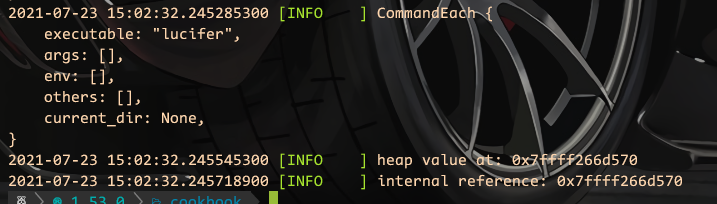
\includegraphics[width=\linewidth]{self_ref_on_heap.png}
  \caption{堆区实现自引用结构}
  \label{fig:self_ref_on_heap}
\end{figure}

这是一个有效的自引用结构,并且,由于heap\_value只是一个指针,对它的移动操作(
比如赋值给其他变量,或者作为参数传递)并不会改变结构本身的地址,所以,self\_ptr
会一直保持有效。但是,这种“固定效果”很容易被打破或者破坏,比如将Box包裹的数据解引用
或者直接替换:
\begin{code-block}{rust}
use std::mem;

fn main() {

    let mut heap_value = Box::new(SelfReferential {
        self_ptr: 0 as *const _,
    });

    let ptr = &*heap_value as *const SelfReferential;
    heap_value.self_ptr = ptr;

    println!("heap value at: {:p}", heap_value);
    println!("internal reference: {:p}", heap_value.self_ptr);

    // break it
    let stack_value = mem::replace(&mut *heap_value, SelfReferential {
        self_ptr: 0 as *const _,
    });

    println!("value at: {:p}", &stack_value);
    println!("internal reference: {:p}", stack_value.self_ptr);

    let hp = *heap_value;
    println!("heap value at: {:p}", &hp);
    println!("internal reference: {:p}", &(hp.self_ptr));
}

struct SelfReferential {
    self_ptr: *const Self,
}
\end{code-block}
则可以观察到,对应的结构体的内存地址全部发生了变化:
\begin{figure}[H]
  \centering
  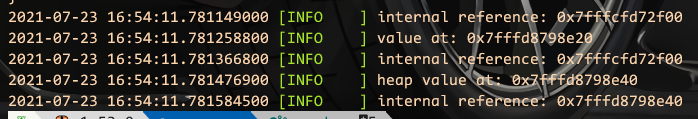
\includegraphics[width=\linewidth]{self_ref_on_heap_break.png}
  \caption{自引用结构的内存破坏}
  \label{fig:self_ref_on_heap_break}
\end{figure}

\begin{warn}
这种操作是比较危险的,利用mem::replace函数,将原本由堆分配的值替换成新的结构体实例,
即将原始的heap\_value移动到了栈区,此时,self\_ptr变成了悬空指针,仍然指向了原始的
堆区地址,因此,使用堆区分配的方式,并不足以保障自引用结构的安全。
\end{warn}

造成上述问题的根本原因在于Box<T>允许开发者获得一个针对在堆上分配的T的\&mut T的引用,
这使得利用诸如mem::replace/mem::swap这样的函数通过\&mut T实现对堆区数据进行修改
成为可能,从而使得在堆区分配的值失效。为此,针对自引用结构,禁止创建\&mut T这样
的引用是必须的。

Rust的Pinging API通过使用Pin Wrapper类型以及Unpin这个标记型Trait来提供了一种可靠
的解决方案。这种解决方案背后的思路是,搜集所有Pin或者需要进行固定的结构体/类型的
特定方法——这些特定的方法可以通过获取可变的引用(\&mut)来获取被Pin Wrapper包括的
实际类型的值——并将这些方法在Unpin Trait上进行实现;Unpin Trait是一个自动的Trait,
除了那些需要进行显式的选择退出类型,其他所有的类型都实现了它;通过标记自引用结构是
实现的显式选择退出Unpin,这将导致没有任何一个安全(safe)的方法可以从Pin<Box<T>>
类型当中获取一个合法有效的可变引用(\&mut T),因此,这种方式实现的自引用结构,
其内部可以保证内部的自引用一直有效。

利用这种思路,我们可以将之前编写的自引用结构进行改写:
\begin{code-block}{rust}
use core::marker::PhantomPinned;

struct SelfReferential {
    self_ptr: *const Self,
    _pin: PhantomPinned,
}
\end{code-block}

通过在结构体当中插入一个类型为PhantomPinned的字段,我们实现了结构体的选择退出。
PhantomPinned类型是一个零字节大小(不占据内存空间)的标记类型,其作用在于标记对应
的数据类型不实现Unpin Trait。由于Auto Trait的工作机制,该类型(PhantomPinned,
即没有实现Unpin)的标记字段足以影响整个结构体,使之不受Unpin Trait的影响。另外
需要改动的地方,则是将上述的Box<SelfReferential>修改为Pin<Box<SelfReferential>>
类型,实现这个改动,最简单的方式就是用Box::pin,如下:
\begin{code-block}{rust}
let mut heap_value = Box::pin(SelfReferential {
    self_ptr: 0 as *const _,
    _pin: PhantomPinned,
});
\end{code-block}
由于PhantomPinned是零字节大小的类型,因此只需要使用类型名初始化对应的字段即可。
再来看看修正之后的完整代码:
\begin{code-block}{rust}
use std::mem;
use std::marker::PhantomPinned;

fn main() {

    let mut heap_value = Box::pin(SelfReferential {
        self_ptr: 0 as *const _,
        _pin: PhantomPinned,
    });

    let ptr = &*heap_value as *const SelfReferential;
    heap_value.self_ptr = ptr;

    println!("heap value at: {:p}", heap_value);
    println!("internal reference: {:p}", heap_value.self_ptr);

    // break it
    let stack_value = mem::replace(&mut *heap_value, SelfReferential {
        self_ptr: 0 as *const _,
        _pin: PhantomPinned,
    });

    println!("value at: {:p}", &stack_value);
    println!("internal reference: {:p}", stack_value.self_ptr);
}

struct SelfReferential {
    self_ptr: *const Self,
    _pin: PhantomPinned,
}
\end{code-block}
如果对上述代码进行编译,编译器将提示下列的错误:
\begin{figure}[H]
  \centering
  
\includegraphics[width=\linewidth]{self_ref_pinned.png}
  \caption{Pinned的自引用结构}
  \label{fig:self_ref_pinned}
\end{figure}

这些错误实际上都是由于Pin<Box<SelfReferential>>这种数据类型包含了PhantomPinned这种
特殊的标记数据类型,从而使得整个类型不再实现DerefMut这个Trait,进而导致了错误的发生。
但这实际上正是我们想要的结果:因为DerefMut Trait本身就会返回一个\&mut T的可变引用,
现实的需求要求这种情况的发生。

但是,这也带来了一个额外的负面作用:无法对结构体当中的self\_ptr进行有效的初始化。
这是因为编译器无法区分\&mut引用的有效和无效使用。为了让初始化操作正常进行,使用不安
全的get\_unchecked\_mut方法便成了不多的选择之一:
\begin{code-block}{rust}
unsafe {
    let mut_ref = Pin::as_mut(&mut heap_value);
    // mut_ref.get_unchecked_mut().self_ptr = ptr; 效果和下面相同
    Pin::get_unchecked_mut(mut_ref).self_ptr = ptr;
}
\end{code-block}

get\_unchecked\_mut函数是Pin<\&mut T>而不是Pin<Box<T>>上的函数,因此需要进行一次
转换(as\_mut),并且该函数返回一个\&mut T,因此,可以利用其返回结果进行修改。
到目前为止,还剩下的错误则是replace操作,但该操作试图将在堆区上分配的值移动到栈区,
这会直接破坏存储在self\_ptr当中的自引用。使用Pin以及退出Unpin则可以防止这个移动操作,
从而安全的使用自引用结构。不过,也应当看到,在目前的Rust版本当中,由于编译器还不能
证明或者解决自引用的创建/初始化是安全的,因此,还需要上述的unsafe操作块。

虽然上述的方式可以很好的解决我们所面临的问题,不过由于所有的操作都是在堆上进行,
而堆区内存的分配显而易见的带来了性能损耗。所幸,Rust的Pinning API也允许创建Pin<\&mut T>
这种在内存栈上分配的实例。和Pin<Box<T>>拥有T类型的所有权不同,Pin<\&mut T>只是
针对T的一个临时引用,这使得在内存栈上的Pin变得更加复杂。更重要的是,一个Pin<\&mut T>
必须保证被引用的T在整个生命周期当中都保持固定,但是,这对于基于栈内存的变量是难以
验证的,因此,通常情况下,\colorblock{并不推荐在栈内存上使用Pinning API进行变量固定}。

有了以上的了解之后,利用Pin对之前的示例进行改写:
\begin{code-block}{rust}
use std::mem;
use std::marker::PhantomPinned;
use std::pin::Pin;
use std::future::{self,Future};
use std::task::{Context, Poll};
struct StringLen<F> {
    inner_future: F,
    _pin: PhantomPinned,
}
impl<F> Future for StringLen<F> where F: Future<Output = String> {
    type Output = usize;
    fn poll(mut self: Pin<&mut Self>, cx: &mut Context<'_>) -> Poll<Self::Output> {
        match self.as_mut().poll(cx) {
            Poll::Ready(s) => Poll::Ready(s),
            Poll::Pending => Poll::Pending,
        }
    }
}
fn string_len(string: impl Future<Output = String>)
    -> impl Future<Output = usize>
{
    StringLen {
        inner_future: string,
        _pin: PhantomPinned,
    }
}
fn file_len() -> impl Future<Output = usize> {
    let file_content_future = async_read_file("foo.txt");
    string_len(file_content_future)
}
fn async_read_file(name: &str) -> impl Future<Output = String> {
    future::ready(String::from(name))
}
\end{code-block}
虽然这只是一个对Future的简单模拟,但总算是可以编译通过了。正如在上面看到的一样,
async/await创建的实例通常是自引用结构,通过将实例(self)封装在Pin当中,使之退出
Unpin,可以确保对应的Future在轮询调用当中不会在内存当中发生移动,从而确保了所有
的内部引用仍然有效。

不过需要注意的是,在第一次调用轮询poll之前对future进行移动是可以的。这是因为Future
属于懒加载的一种模式,在第一次调用轮询前什么也不会做。因此,编译器生成的状态机
通常情况下只包含了函数参数,但是不包括内部引用。为了轮询调用poll,首先需要将Future
封装到Pin当中,来保证其在内存当中不会发生移动。另外,由于栈区的pinning更加难以操作,
通常情况下,使用Box::Pin配合Pin::as\_mut是一个最优选择。

\subsection{执行器(Executors)与唤醒器(Wakers)}
使用async/await,可以以完全异步的方式处理Future。不过,正如上面所介绍的,Future
在被轮询之前什么也不做。这意味着我们必须在某些时候对它们调用轮询(即唤醒),否则
异步代码永远也不会执行。

对于单个Future,我们总是可以使用上面描述的循环手动等待每个future。然而,这种方法
效率非常低,并且对于包含了大量Future的程序来说也不实用。这个问题最常见的解决方案
是定义一个全局执行器,该执行器负责轮询系统中的所有后续操作,直到它们完成为止。

执行器的目的在于允许Future成为一个独立的任务,然后对这些Future进行轮询,直到这些
Future(任务)全部完成为止。因此,全局的执行器最大的优点在于:当Future返回Poll::Pending
时,执行器可以在不同的Future之间进行切换。由于异步操作总是以并行/并发的方式执行的,
因此CPU通常一直处于忙碌状态,提高了资源的利用率。

由于Rust的标准库并没有提供Future的标准执行器,因此,执行器绝大部分是第三方的类库
进行实现的。这些类库在实现执行器时,通常利用了现代的多核技术,一般是创建一个线程
池来充分利用所有的CPU核。为了避免一次次轮询Future带来的开销,执行器通常和Future
支持的唤醒器(Waker)一起工作。

唤醒器的思路是,一个特殊的waker类型当作参数封装在Context类型当中传递给poll调用,
并且这个类型由执行器创建,异步任务可以使用这个waker表示任务结束。因此执行器可以
不再针对Poll::Pending的Future调用poll操作,而是等待相应的waker通知,比如之前的
简单例子:
\begin{code-block}{rust}
async fn write_file() {
    async_write_file("foo.txt", "Hello").await;
}
\end{code-block}
函数async\_write\_file异步地将字符串“Hello”写入foo.txt文件,由于硬盘写入需要一些
时间,因此针对Future的第一个poll调用可能会返回poll::Pending。不过,硬盘驱动程序
可以在内部存储传递给poll调用的Waker,并在文件被写入磁盘时使用它通知执行程序(执行者,Executor)。
通过这种方式,执行器在收到唤醒器通知之前就不需要浪费任何时间再次对Future进行poll调用。

虽然Rust并没有自己提供的标准执行器和唤醒器,但是可以利用Rust提供的标准库,自己
实现一个简单的执行器和唤醒器!在实现自己的执行器和唤醒器之前,我们需要了解一下多任务。
在操作系统当中,并行/并发都涉及到了多任务处理。而多任务处理主要有2种方式:抢占式
多任务以及协作式多任务。抢占式多任务依赖于操作系统在运行的任务之间强制切换,而
协作式多任务则要求任务通过yield或者同类型的操作定期自动放弃对CPU的控制。协作方法
的最大优点是任务可以自己保存状态,从而实现更有效的上下文切换,并使任务之间共享
相同的调用堆栈成为可能。而Rust的Future和async/await是合作多任务模式,因此,在实
现自己的执行器和唤醒器时,需要注意下列的需求:
\begin{itemize}
  \item 每一个添加到执行器当中future都是协作式任务(task,有些时候会将future直接当作task看待)
  \item Future不是通过yield操作,而是通过返回Poll::Pending或Poll::Ready来放弃对CPU的控制权
  \begin{itemize}
    \item 没有任何操作可以强制future放弃CPU的控制权,除非future永远不从poll操作返回,比如在无限循环当中自旋(spinning lock)
    \item 每一个future都可以或者可能阻塞执行器当中的其他future的执行过程,需要保证每个future都不是“恶意的”
  \end{itemize}
  \item Future会在内部存储所有在下一次poll调用时会被使用到的状态/状态。通过async/await,编译器会自动检测所需要的所有变量,并将其存储在生成的状态机当中
  \begin{itemize}
    \item 通常只保存所需要的最少变量
    \item 由于poll操作返回时会放弃对应的堆栈区,因此可以使用相同的堆栈区去轮询其他的future
  \end{itemize}
\end{itemize}

在接下来的示例当中将使用标准库(std)来实现一个Future的完成运行流程,包括执行器和
唤醒器的实现。首先编写我们的异步函数:
\begin{code-block}{rust}
async fn async_number() -> u32 {
    42
}
async fn example_task() {
    let number = async_number().await;
    println!("async number: {}", number);
}
\end{code-block}

async\_number是一个异步函数,Rust编译器会将其在内部转换成状态机。由于该函数只是
返回一个数字,所以在第一次轮询操作(poll)结束时该函数最终会直接返回一个Poll::Ready(42)。
example\_task类似,只是该函数需要等待async\_number的返回结果。Future已经通过async/await
生成好了(example\_task返回的),如果想要运行这个future,则需要对它调用poll操作,
直到接收到Poll::Ready所代表的完成信号为止。因此,现在需要一个任务管理器:
\begin{code-block}{rust}
use std::future::Future;
use std::pin::Pin;
pub struct Task {
    future: Pin<Box<dyn Future<Output = ()>>>,
}
\end{code-block}
该任务(task)结构体是一个包裹类型,包裹了一个具有Pinned属性的、在堆上动态分配的动态Future
类型,并且,这个Future类型的输出类型(即关联类型Output)为空类型。该结构体有如下特点:
\begin{itemize}
  \item Future的关联类型返回(),表示任务(即future)不会返回任何结果,我们的目的仅仅只是使得这个future可以正常运行
  \item dyn关键字表示存储在Box当中的是一个Trait对象,意味着future的方法是动态分配的,这使得在Task类型当中存储不同类型的Future成为可能,也使得可以创建多个不同的任务(future)
  \item Pin保证包裹的对象不能在内存当中移动,防止状态机产生的自引用结构失效
\end{itemize}

接下来实现Task结构体的初始化(new)方法以及poll方法,由于需要使用Task结构体轮询
存储在内存当中的future,因此,poll方法是必需的:
\begin{code-block}{rust}
impl Task {
    pub fn new(future: impl Future<Output = ()> + 'static) -> Task {
        Task {
            future: Box::pin(future),
        }
    }
    fn poll(&mut self, context: &mut Context) -> Poll<()> {
        self.future.as_mut().poll(context)
    }
}
\end{code-block}
new方法接收一个关联类型为()的任意Future,并且通过Box::pin将其在内存当中固定,然后
封装在Task结构体当中进行返回。需要注意,这里需要一个static的生命周期,因为返回的
Task可以在任意时间存在,所以,Future也需要在任意时间内有效。

由于Future Trait的poll方法定义为\codeinline{rust}{fn poll(self: Pin<&mut Self>, cx: &mut Context<'_>) -> Poll<Self::Output>;},
因此,首先需要通过as\_mut方法将self.future从\codeinline{rust}{Pin<Box<T>>}(Box::pin的返回)转换成
Pin<\&mut T>,然后对转换之后的future调用poll函数。由于Task::poll方法应该只由稍后
创建的执行器调用,因此需要将该函数设置为私有模式。

接下来构造一个简单的执行器:
\begin{code-block}{rust}
pub struct SimpleExecutor {
    task_queue: VecDeque<Task>,
}

impl SimpleExecutor {
    pub fn new() -> SimpleExecutor {
        SimpleExecutor {
            task_queue: VecDeque::new(),
        }
    }
    pub fn spawn(&mut self, task: Task) {
        self.task_queue.push_back(task)
    }
}
\end{code-block}
该执行器包含了一个双端队列,通过spawn方法在队列尾部插入新的任务,从队列头部弹出下一个
任务进行执行。

为了调用Future的poll方法,接下来需要创建一个Context类型的对象,这个对象封装了一个
唤醒器(Waker)来监听Future的完成状态。为此,首先创建一个RawWaker实例,它定义了
不同Waker方法的实现,然后使用Waker::from\_raw函数将其转换为Waker。
\begin{code-block}{rust}
fn dummy_waker() -> Waker {
    unsafe { Waker::from_raw(dummy_raw_waker()) }
}

fn dummy_raw_waker() -> RawWaker {
    fn no_op(_: *const ()) {}
    fn clone(_: *const ()) -> RawWaker {
        dummy_raw_waker()
    }
    let vtable = &RawWakerVTable::new(clone, no_op, no_op, no_op);
    RawWaker::new(0 as *const (), vtable)
}
\end{code-block}

RawWaker类型需要显式地定义一个函数虚表(vtable),这个虚表当中需要包含RawWaker被
复制(clone),唤醒(woken)以及销毁(dropped)时应该被调用的函数。这几个函数的
形式应当如下:
\begin{code-block}{rust}
clone: unsafe fn(*const ()) -> RawWaker,
wake: unsafe fn(*const ()),
wake_by_ref: unsafe fn(*const ()),
drop: unsafe fn(*const ()),
\end{code-block}
这个虚表的布局是由RawWakerVTable类型定义的,每个函数都接收一个*const()参数,它
基本上是一个类型擦除(不关心)的\&self指针,指向某个结构体,例如分配在堆上。使用*const()
指针而不是正确的引用的原因是RawWaker类型应该是非泛型的,但仍然应该支持任意类型。

一般情况下,RawWaker是为包装在Box或Arc类型中的某些在堆区分配的结构所创建的。
对于这类类型,可以使用Box::into\_raw之类的方法将Box<T>转换成*const T指针,而这种
类型的指针可以被转换为一个匿名*const()指针,并传递给RawWaker::new方法。由于每个
虚表函数都接收相同的*const()作为实参,因此函数可以安全地将指针强制转换回Box<T>
或者是一个\&T来操作它。但是这样的操作会涉及到指针的强制转换,因此整个
过程实际上是非常危险的,非常容易导致错误的行为。\colorblock{除非必要,不建议手动
创建RawWaker}。

在上述的代码当中,首先定义了2个内部函数no\_op和clone。这2个函数都接收一个*const()指针
作为参数,不同的是,no\_op不做任何处理和操作,而clone函数通过调用dummy\_raw\_waker
返回一个新的RawWaker。接下来使用这两个函数来创建一个最小的RawWakerVTable:clone函数
用于clone操作,no\_op函数用于所有其他操作。

虚表创建成功之后,再使用RawWaker::new函数来创建RawWaker。由于虚表函数并没有使用第一个
参数,因此,在创建RawWaker时,第一个参数使用了空指针作为代替(0 as *const())。

有了唤醒器,我们就可以在执行器上实现一个run方法来调用这个唤醒器。最简单的运行方法
就是在循环中反复轮询所有排队的任务,直到全部完成。注意,这并不是很有效,因为它没
有利用Waker类型的通知机制,不过这并不影响它的正常运行,如下代码所示:
\begin{code-block}{rust}
impl SimpleExecutor {
    pub fn run(&mut self) {
        while let Some(mut task) = self.task_queue.pop_front() {
            let waker = dummy_waker();
            let mut context = Context::from_waker(&waker);
            match task.poll(&mut context) {
                Poll::Ready(()) => {} // task done
                Poll::Pending => self.task_queue.push_back(task),
            }
        }
    }
}
\end{code-block}
该函数使用while-loop来处理task\_queue中的所有任务。对于每个任务,它首先通过
由dummy\_waker函数返回的Waker实例来创建一个Context类型的实例,然后对每个任务
调用poll进行轮询,如果poll方法返回poll::Ready,则任务结束,接着下一个任务;
如果任务仍然是Poll::Pending,我们将它再次添加到队列的后面,以便在后续循环迭代中
再次轮询它,直到该任务执行完毕。

接下来看一下完整的代码:
\begin{code-block}{rust}
use std::collections::VecDeque;
use std::future::Future;
use std::pin::Pin;
use std::task::{Context, Poll,Waker, RawWaker,RawWakerVTable};
pub struct Task {
    future: Pin<Box<dyn Future<Output = ()>>>,
}
impl Task {
    pub fn new(future: impl Future<Output = ()> + 'static) -> Task {
        Task { future: Box::pin(future), }
    }
    fn poll(&mut self, context: &mut Context) -> Poll<()> {
        self.future.as_mut().poll(context)
    }
}
pub struct SimpleExecutor { task_queue: VecDeque<Task>, }
impl SimpleExecutor {
    pub fn new() -> SimpleExecutor {
        SimpleExecutor { task_queue: VecDeque::new(), }
    }
    pub fn spawn(&mut self, task: Task) {
        self.task_queue.push_back(task)
    }
    pub fn run(&mut self) {
        while let Some(mut task) = self.task_queue.pop_front() {
            let waker = dummy_waker();
            let mut context = Context::from_waker(&waker);
            match task.poll(&mut context) {
                Poll::Ready(()) => {} // task done
                Poll::Pending => self.task_queue.push_back(task),
            }
        }
    }
}
fn dummy_waker() -> Waker {
    unsafe { Waker::from_raw(dummy_raw_waker()) }
}
fn dummy_raw_waker() -> RawWaker {
    fn no_op(_: *const ()) {}
    fn clone(_: *const ()) -> RawWaker { dummy_raw_waker() }
    let vtable = &RawWakerVTable::new(clone, no_op, no_op, no_op);
    RawWaker::new(0 as *const (), vtable)
}
async fn async_number() -> u32 { 42 }
async fn example_task() {
    let number = async_number().await;
    println!("async number: {}", number);
}
fn main() {
    let mut executor = SimpleExecutor::new();
    executor.spawn(Task::new(example_task()));
    executor.run();
}
\end{code-block}

到此为止,Future的整体运行机制以及执行器的实现思路已经明白无误的剖析在了面前,
并且上述代码全部使用Rust的标准库(std)实现的。从上面的例子可以看到,Rust的标准
库针对Future只保证下列的必需条件:
\begin{itemize}
  \item 标准的Future Trait
  \item 一个合乎常理的方法创建任务,并且可以通过async/await对Future进行暂停/恢复
  \item 标准的Waker Trait,可以唤醒暂停的Future
\end{itemize}
但是,\colorblock{并不包含异步任务的执行}。

\begin{note}
Future,Waker以及相关的Task,在标准库(std)当中存在,在核心库(core)当中也存在,
并且,std和core当中的定义和实现是一模一样的,因此,async/await以及Future等异步
操作不仅可以用于普通的Rust开发,也同样可以用于没有std模式的嵌入式开发,甚至是操作
系统开发。除此之外,其他常用的异步开发框架,比如futures,async-std等,其内部定义
的Future,Waker以及Task等Trait,和Rust std都是完全相同的。这些类库当中的相关Trait
完全等价,使用时无需进行转换。不过,确切的说,除了core当中的Future定义,
Future的定义只有2类:一种是std当中的,而另外一种则是future-rs提供的futures::future::Future,
其中future-rs当中的是最原始的定义,而为了给Rust提供异步支持,才将future-rs当中的
相关定义移入到了std当中,也就是说,std当中的Future实际上是future-rs的最小子集。
而同样的,async-std、tokio等类库当中的Future实现,实际上也是future-rs的重新导出。
\end{note}
\subsection{Future补遗}
\subsubsection{胖指针与虚表}
Rust当中也存在指针,但是存在一些特殊的指针,比如下面的代码:
\begin{code-block}{rust}
use std::mem::size_of;
trait SomeTrait {}
fn main() {
    info!("======== The size of different pointers in Rust: ========");
    info!("&dyn Trait:-----{}", size_of::<&dyn SomeTrait>());
    info!("&[&dyn Trait]:--{}", size_of::<&[&dyn SomeTrait]>());
    info!("Box<Trait>:-----{}", size_of::<Box<dyn SomeTrait>>());
    info!("&i32:-----------{}", size_of::<&i32>());
    info!("&[i32]:---------{}", size_of::<&[i32]>());
    info!("Box<i32>:-------{}", size_of::<Box<i32>>());
    info!("&Box<i32>:------{}", size_of::<&Box<i32>>());
    info!("[&dyn Trait;4]:-{}", size_of::<[&dyn SomeTrait; 4]>());
    info!("[i32;4]:--------{}", size_of::<[i32; 4]>());
}
\end{code-block}
如果执行上述代码,我们会发现每个指针的大小都不一样:
\begin{figure}[H]
  \centering
  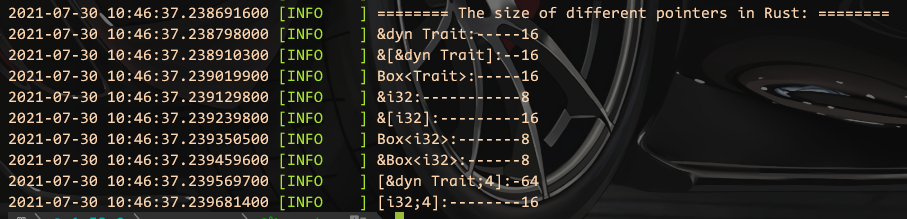
\includegraphics[width=\linewidth]{fat_pointer.png}
  \caption{不同类型的指针}
  \label{fig:fat_pointer}
\end{figure}
有的是8字节大小(64位系统的默认指针大小),而有的则是16字节。这些16字节的指针,就是
所谓的胖指针(Fat Pointer)。胖指针通常携带了额外的信息:
\begin{itemize}
  \item \&[i32]以及[i32;4]
  \begin{itemize}
    \item 前8个字节是指向数组中第一个元素的实际指针,或 slice 引用的数组的一部分
    \item 后8个字节,则表示的是切片以及数组的长度
  \end{itemize}
  \item \&dyn Trait
  \begin{itemize}
    \item 前8个字节指向Trait对象的数据段(data)
    \item 后8个字节指向Trait对象的虚表(vtable)
  \end{itemize}
\end{itemize}
正是由于虚表和胖指针的存在,才使得Rust的Trait如同Java的Interface、C++的虚函数、
C的函数指针一样,可以针对不同的类型进行操作。我们可以直接使用代码来模拟Trait是如何
使用胖指针和虚表来实现动态分发(针对不同的类型使用相同的方法定义)的:
\begin{code-block}{rust}
use std::mem::transmute;
trait SomeTrait {
    fn add(&self) -> i32;
    fn sub(&self) -> i32;
    fn mul(&self) -> i32;
}
// 结构体的内存布局和对齐方式采用兼容C语言的模式进行
#[repr(C)]
struct FatPointer<'a> {
    // 使用data指向Trait的数据段
    data: &'a mut Data,
    // 指向Trait的vtable段。由于需要传入长度和对齐等字面值,
    // 因此最容易的方法是使用无符号数的指针
    vtable: *const usize,
}
struct Data {
    a: i32,
    b: i32,
}
fn add(s: &Data) -> i32 {
    s.a + s.b
}
fn sub(s: &Data) -> i32 {
    s.a - s.b
}
fn mul(s: &Data) -> i32 {
    s.a * s.b
}
fn main() {
    let mut data = Data { a: 3, b: 4 };
    // 使用vec构造一个类似的虚表结构
    // 虚表(vtable)是具有固定格式的特殊用途的指针数组,
    // 每个元素都有特殊的含义
    let vtable = vec![
        0,  // 指向Drop的指针,这里的0表示NULL/None,即在这个虚表当中没有实现drop函数
        6,  // 虚表的长度
        8,  // 虚表当中元素的对其方式,此处表示按照8字节对齐

        // 从第4个元素开始,表示的是Trait当中定义的字段/方法
        // 这里的字段顺序必须和Trait当中定义的顺序相同
        add as usize, // 函数指针
        sub as usize,
        mul as usize
    ];
    let fat_pointer = FatPointer {
        data: &mut data,
        // 将vtable转换成指针
        vtable: vtable.as_ptr(),
    };
    // 使用transmute将fat_pointer转换成 dyn SomeTrait的对象
    // 等同于 let res: &dyn SomeTrait = unsafe { transmute(fat_pointer) };
    let res = unsafe { transmute::<FatPointer, &dyn SomeTrait>(fat_pointer) };
    info!("{}", res.add());
    info!("{}", res.sub());
    info!("{}", res.mul());
}
\end{code-block}

实际上,上述代码的模拟与Rust标准库的Trait非常类似,可以参考TraitOjbect的定义
\footnote{TraitObject:\url{https://doc.rust-lang.org/std/raw/struct.TraitObject.html}}。
虽然Rust的源代码实现有些区别,但Trait的实现方式,其工作机制和模式,可以通过上述
的代码全部展现出来。

\subsubsection{Future的基本使用方式}
虽然对Future的原理和实现方式有了大致的了解,但是Future的使用方式,还没有进行介绍。
Future基本分为2大类:async/await修饰的普通函数,以及实现Future Trait的结构体。这
2种的类型的使用方式类似,唯一有区别的是,结构体需要实现Future Trait的相关方法,
如下的代码所示:
\begin{code-block}{rust}
use std::task::{Context,Poll};
use std::pin::Pin;
use futures::future::Future;
use futures::executor::block_on;

pub struct Number {
    number: u8,
    polled: bool,
}

impl Number {
    pub fn new(number: u8) -> Self {
       Self {
            number: number,
            polled: false,
       }
    }
}

// 结构体实现Future Trait
impl Future for Number {
    type Output = u8;
    fn poll(
       self: Pin<&mut Self>,
       cx: &mut Context<'_>,
    ) -> Poll<Self::Output> {
        let mut this = self.get_mut();
        if this.polled {
            Poll::Ready(this.number)
        } else {
            // 调用唤醒器,否则调用poll时会直接进入死循环
            cx.waker().wake_by_ref();
            this.polled = true;
            Poll::Pending
        }
    }
}

async fn get_num() -> u8 {
    18
}

async fn outer() -> u8 {
    get_num().await
}

fn main(){
    let num = Number::new(98);
    // 将num对象当作一个future使用
    let res = block_on(num);
    println!("{}", res);
    // 同上
    let num = async { Number::new(100).await };
    let res = block_on(num);
    println!("{}", res);
    // 将异步函数当作future使用,2种不同的使用方式
    //let num = async {get_num().await};
    let num = get_num();
    let res = block_on(num);
    println!("{}", res);
    // 将异步函数当作future使用,2种不同的使用方式
    //let res = async {outer().await};
    let res = outer();
    let res = block_on(res);
    println!("{}", res);
}
\end{code-block}

\section{异步编程的实现方案-async-std}
Async-std是一种Future执行器的实现方案。其基本的使用于futures类似,都是使用block\_on
设置异步任务的阻塞运行。相比于futures,async-std提供了一些扩展功能,比如异步的
计时器等。

常见的使用方式都是相同的:
\begin{code-block}{rust}
use async_std::task::block_on;
pub async fn async_hello() {
    info!("This is the async hello");
}

fn main() {
    let _ = block_on(async_hello());
}

\end{code-block}

不过,async-std也还提供了一种简便的方式,这种方式不再要求使用block\_on进行显式的
阻塞执行,但是,使用这种方式,要求启用async-std的特性
\footnote{关于async-std的特性说明:\url{https://docs.rs/async-std/1.9.0/async_std/\#features}}:
\begin{code-block}{toml}
[dependencies]
async-std = {version = "1.9.0", features = ["attributes"]}
\end{code-block}
只用启用了上述的特性,才可以如下进行使用:
\begin{code-block}{rust}
pub async fn async_hello() {
    info!("This is the async hello");
}

#[async_std::main]
async fn main() {
    async_hello().await;
}
\end{code-block}
上述方式相当于将main函数也当作一个异步函数,而该函数的执行,则是由async-std这个
运行时自己进行相关任务的调度。同样的,如果是在测试函数或者测试用例当中,也可以使用
这种方式:
\begin{code-block}{rust}
pub async fn async_hello() {
    info!("This is the async hello");
}

// 注意,同样需要启用attributes属性,并且,main需要修改为test
#[async_std::test]
async fn test_units() {
    async_hello().await;
}
\end{code-block}

如果是多个异步函数的执行,同样可以使用block\_on或者直接的await方式进行操作,但是,
需要注意的是,如果不加控制,不同的异步操作,默认情况下是串行执行的,比如下面的代码:
\begin{code-block}{rust}
use std::time::Duration;
use async_std;
pub async fn connect_db_fake() -> String {
    async_std::task::sleep(Duration::from_secs(1)).await;
    info!("This is the async connect_db_fake function");
    "connect_db_fake".to_owned()
}

pub async fn open_file_fake() -> String {
    async_std::task::sleep(Duration::from_secs(2)).await;
    info!("This is the async open_file_fake function");
    "open_file".to_owned()
}

fn main() {
    let db_fake = async_std::task::block_on(connect_db_fake());
    let file_fake = async_std::task::block_on(open_file_fake());
    ...
}
\end{code-block}
上述代码当中db\_fake和file\_fake并没有什么直接的关系,二者是完全可以并行执行的,
但是,实际的执行结果是,两行代码总计耗时3秒左右,并没有并行起来。如果想让这些
并没有关联关系的操作完全并行起来,则需要使用futures-rs提供的功能:
\begin{code-block}{toml}
[dependencies]
futures = "0.3.15"
async-std = {version = "1.9.0", features = ["attributes"]}
\end{code-block}
并行的代码修改如下:
\begin{code-block}{rust}
use futures;
fn main() {
    let now = time::Instant::now();
    let (fake_db, fake_file) =
        block_on(futures::future::join(connect_db_fake(), open_file_fake()));
    let elapsed = now.elapsed();
    assert_eq!("open_file", fake_file);
    assert_eq!("connect_db_fake", fake_db);
    println!("All of async function used {:#?} ", elapsed);
    assert!(elapsed > Duration::from_secs(1));
    assert!(elapsed < Duration::from_secs(3));
}
\end{code-block}
并行之后的代码,总体的执行时间取决于耗时最长的任务。当然,如果需要并行多个任务,
可以使用join2,join3,join4和join5等函数。针对常见的函数式编程,比如map-reduce
操作,则可以使用join\_all等方法:
\begin{code-block}{rust}
use futures::future::join_all;
use std::time::{self, Duration};
use std::sync::{Arc, Mutex};
use async_std;
pub async fn get_cities() -> Vec<String> {
    let cities = vec![
        "shanghai".to_owned(),
        "beijing".to_owned(),
        "chongqing".to_owned(),
    ];
    let city_vec = Arc::new(Mutex::new(vec![]));
    let _ = join_all(
        cities
            .into_iter()
            .map(|city| build_city(city_vec.clone(), city)),
    )
    .await;
    return city_vec.lock().unwrap().clone();
}

async fn build_city(city_vec: Arc<Mutex<Vec<String>>>, city: String) {
    async_std::task::sleep(Duration::from_secs(1)).await;
    city_vec
        .lock()
        .unwrap()
        .push(format!("Super City {}", city))
}

fn main() {
    let now = time::Instant::now();
    let res = block_on(get_cities());
    assert_eq!(
        vec![
            "Super City shanghai".to_owned(),
            "Super City beijing".to_owned(),
            "Super City chongqing".to_owned()
        ],
        res
    );
    let used = now.elapsed();
    assert!(used < Duration::from_secs(2));
}
\end{code-block}
注意,join\_all也是并行执行的,其耗费的时间同样取决于耗时最长的任务。

而如果只是需要并行任务当中的某一个或者某几个完成,则需要使用select操作:
\begin{code-block}{rust}
pub async fn fake_select_two() -> u8 {
    let future1 = async {
        // 该future一直是pending状态,永远不会返回
        future::pending::<()>().await;
        1
    };
    let future2 = async { future::ready(2).await };
    // 针对select操作,所有的future都必须使用pin_mut
    pin_mut!(future1);
    pin_mut!(future2);
    match future::select(future1, future2).await {
        // select返回(future的Output,另一个future)
        Either::Left((value1, _ignore_future)) => value1,
        Either::Right((value2, _ignore_future)) => value2,
    }
}
\end{code-block}

\begin{note}
Join,join\_all以及join系列的函数和join!这个宏,以及select函数和select!宏,都
包含在futures-rs这个类库当中(tokio当中也有),但是,这些函数以及宏定义,是兼容
目前所有的异步类库的。因此,可以在async-std以及tokio当中使用。
\end{note}

需要注意的是,异步任务(包括async-std、futures以及tokio等)通常是并行运行,但是
这个“并行”的基础是\colorblock{通过共享一个执行线程实现的}。这就意味着阻塞一个操作系统(std)
线程的操作,比如std::thread::sleep将停止所有共享该线程的任务的执行,无法和
async-std的并行模型很好的配合。因此,下列代码在执行过程当中,实际上是串行阻塞式
的运行的:
\begin{code-block}{rust}
task::block_on(async {
    // this is std::fs, which blocks
    std::fs::read_to_string("test_file");
})
\end{code-block}

针对文件系统的异步io,async-std提供了与std::fs兼容的async\_std::fs进行异步化:
\begin{code-block}{rust}
use async_std::fs::File;
use async_std::{io::{self, prelude::WriteExt}};
pub async fn async_file_opts() -> io::Result<()> {
    let mut file = File::create("a.txt").await?;
    Ok(file.write_all(b"hello world").await?)
}
\end{code-block}

同样是由于Rust的异步实现都是通过共享线程实现的,因此,必然会带来这样的问题:
有的异步任务属于定时任务,需要定期的执行,如果通过普通的sleep操作进行控制权
让出,必然会阻塞当前线程的运行,使得异步操作失败。针对这种问题,async-std提供
了自己的定时器解决方案,只不过,这个定时器方案需要启用async-std的unstable特性:
\begin{code-block}{rust}
[dependencies]
async-std = {version = "1.9.0", features = ["attributes", "unstable"]}
\end{code-block}
而代码则需要进行如下的变化:
\begin{code-block}{rust}
use std::time::Duration;
use async_std::stream::{self, StreamExt};

fn main() {
    // 生成一个定时器stream,用于定时发送提示
    let mut intvl = stream::interval(Duration::from_secs(1));
    let mut count = 0;
    // while let Some(_) = intvl.next().await {
    while let Some(_) = block_on(intvl.next()) {
        count += 1;
        if count > 5 {
            break;
        }
        println!("{} seconds elapsed ", count);
    }
}
\end{code-block}
通过在async-std的运行时内部利用stream实现一个定时器,可以很好的和当前线程进行
合理的分离,使得异步的定时任务成为可能。而在上面的代码当中,出现了一个关键字,
或者说是新的概念:stream。Stream实际上对应的是Rust当中迭代器的概念。在目前通用的
Rust异步编程类库当中,Stream的定义和实现上都是类似的,以futures-rs为例,其定义
大致如下\footnote{来源:\url{https://docs.rs/futures/0.3.16/futures/stream/trait.Stream.html}}
\begin{code-block}{rust}
pub trait Stream {

    type Item;

    fn poll_next(
        self: Pin<&mut Self>,
        cx: &mut Context<'_>
    ) -> Poll<Option<Self::Item>>;

    fn size_hint(&self) -> (usize, Option<usize>) { ... }
}
\end{code-block}
而async-std当中的Stream定义则稍微有些不同,不过,核心部分是类似的\footnote{async:\url{https://docs.rs/async-std/1.9.0/async_std/stream/trait.Stream.html}}:
\begin{code-block}{rust}
pub fn poll_next(
    self: Pin<&mut Self>,
    cx: &mut Context<'_>
) -> Poll<Option<Self::Item>>
\end{code-block}
并且,async-std也特意说明了,async-std当中的Stream实际上是对futures-rs当中的Stream的重新
导出(re-export),因此,二者在本质上并没有什么区别。和普通future相比,Stream在实现
上实际上并没有太大的区别,在编译器内部也是通过状态机或者生成器实现的。比如,一个
简单的Stream实现如下:
\begin{code-block}{rust}
use std::pin::Pin;

use async_std::prelude::*;
use async_std::stream;
use async_std::task::{Context, Poll};

fn increment(
    s: impl Stream<Item = i32> + Unpin,
) -> impl Stream<Item = i32> + Unpin {

    struct Increment<S>(S);

    impl<S: Stream<Item = i32> + Unpin> Stream for Increment<S> {

        type Item = S::Item;

        fn poll_next(
            mut self: Pin<&mut Self>,
            cx: &mut Context<'_>,
        ) -> Poll<Option<Self::Item>> {

            match Pin::new(&mut self.0).poll_next(cx) {
                Poll::Pending => Poll::Pending,
                Poll::Ready(None) => Poll::Ready(None),
                Poll::Ready(Some(item)) => Poll::Ready(Some(item + 1)),
            }
        }
    }

    Increment(s)
}

let mut s = increment(stream::once(7));
\end{code-block}
只不过,在真实的生产环境当中,stream的使用并没有这么复杂:
\begin{code-block}{rust}
// 下列2行任选其一即可
// use futures::stream::{self, StreamExt};
use async_std::stream::{self, StreamExt};

fn test_stream_future() {
    // futures-rs的用法
    //let mut streamf = stream::iter(1..=10);

    // async-std的用法
    let mut streamf = stream::from_iter(1..=10);

    let res = block_on(streamf.next());
    assert_eq!(Some(1), res);

    // 迭代器消费了一个元素
    let all_item = block_on(streamf.collect::<Vec<u8>>());
    assert_eq!(vec![2, 3, 4, 5, 6, 7, 8, 9, 10], all_item);
}
\end{code-block}
可以看到,futures-rs/async-std的stream和普通的迭代器基本没有太大的差别。而上面
的定时器,可以看作是async-std实现的一个stream特例。
\begin{critical}
默认情况下,针对有限的stream(即数据有限的迭代器),标准迭代器的所有方法都可以
使用,但是,针对无限的stream(即数据无限的迭代器),那些需要遍历所有stream当中
的元素的方法或者函数,则应当禁止使用,否则可能造成用于无法返回,比如下面的例子:
\begin{code-block}{rust}
// 构造一个无限的流,流当中的每个元素都是1
let ones = async_std::stream::repeat(1);
// 无法结束,因为min函数需要迭代流当中的所有元素
// 这是无法完成的操作
let least = ones.min().await.unwrap();
println!("The smallest number one is {}.", least);
\end{code-block}
\end{critical}

针对Rust常用的多线程通信方案channel,async-std以及futures-rs同样提供了对应的异步方案:
\begin{code-block}{rust}
use async_std::channel::{unbounded, RecvError, TryRecvError};
async fn test_async_channel() {
    let (sender, recver) = unbounded(); // 创建无缓冲的channel,如果是有缓冲
                                        // let (sender, recver) = bounded(2);
    assert_eq!(sender.send(1).await, Ok(()));
    assert_eq!(recver.recv().await, Ok(1));
    assert_eq!(recver.try_recv(), Err(TryRecvError::Empty));
    // 不管是unbounded还是bounded的channel,如果sender
    // 没有继续发送消息,也没有进行关闭,但是,继续使用
    // recver.recv() 操作,会导致对应的任务进入死锁状态
    // 无法继续向后执行,因此,下面的代码需要注意
    // assert_eq!(recver.recv().await, Ok(_));
    drop(sender);
    assert_eq!(recver.try_recv(), Err(TryRecvError::Closed));
    assert_eq!(recver.recv().await, Err(RecvError));
}
\end{code-block}
这些channel的使用方式和标准库当中的channel基本类似,唯一的区别可能就是他们是异步
方式。

\begin{note}
在async-std以及其他的异步执行器出来之前,使用最多的是future-rs。Future-rs提供了
Rust异步编程的所有完整实现,包括贡献了async/await关键字。不过,由于其他的异步执行器
发展比较快,生态比较完善,因此,相比较而言,future-rs使用并不是特别多。尤其是,
针对执行器,迭代器以及channel等的实现上,async-std以及tokio等都非常灵活和完善,
并且和future-rs的使用方式相兼容,因此,直接使用future-rs当作异步执行器并不是特别
常见,而是使用future-rs的其他功能。而async-std的目的是提供一个异步的Rust标准库(std)
的实现方案,在目前的版本当中,Rust的std方法,大部分都可以在\colorblock{async-std当中
找到对应的异步实现},因此可以考虑在大多数的异步环境当中,直接使用async-std替换
对应的标准库。
\end{note}

\section{异步编程的实现方案-tokio}
作为目前使用最为广泛的异步开发库之一,Tokio和async-std类似,但更多是被async-std
所借鉴,包括直接异步的方式使用,以及显式的block方式使用,都是tokio首创的。使用
使用tokio也需要在项目的Cargo.toml当中引入相关的依赖:
\begin{code-block}{toml}
[dependencies]
futures = "0.3.15"
tokio = { version = "1.10.0", features = ["full"]}
\end{code-block}

Tokio常见的用法和async-std类似,比如直接使用block的方式:
\begin{code-block}{rust}
let rt = tokio::runtime::Runtime::new().unwrap();
rt.block_on(open_file_fake());
\end{code-block}
注意,和async-std以及futures-rs稍有不同,tokio具有明确的运行时的概念。

当然,也可以使用宏定义的方式:
\begin{code-block}{rust}
#[tokio::main]
async fn main() {
    let blocking_task = tokio::task::spawn_blocking(|| {
    });
    blocking_task.await.unwrap();
}
\end{code-block}
同样的,针对于测试,tokio也提供了对应的宏定义支持:
\begin{code-block}{rust}
#[tokio::test]
async fn test_block() {
    let block_task = tokio::task::spawn_blocking(|| {});
    block_task.await.unwrap();
}
\end{code-block}
Tokio不仅可以用于标准的Rust开发,同样可以应用于嵌入式开发;不仅可以用于普通的异步
功能开发,同样可以用于异步文件IO操作;不仅可以用于网络开发,同样可以应用于多线程
开发。
\subsection{异步文件IO}
同async-std类似,tokio同样提供了文件系统的异步io支持,包括文件/夹的创建、删除
以及其他的操作,tokio都提供了同std库相同或者相近的功能。在实际的异步开发当中,
可以直接使用这些tokio所提供的函数或者功能替代std的相关函数或者功能。

比如遍历指定路径下的所有内容(非递归):
\begin{code-block}{rust}
use tokio::fs;
use tokio::io::{AsyncBufReadExt, AsyncReadExt, AsyncWriteExt, BufReader};
pub async fn fs_direntry_tokio(
    path: &str
) -> Result<Vec<OsString>, std::io::Error> {
    let mut vec_path = vec![];
    let mut entries = fs::read_dir(path).await?;
    while let Some(entry) = entries.next_entry().await? {
        vec_path.push(entry.file_name());
    }
    Ok(vec_path)
}
\end{code-block}

比如递归方式创建指定路径:
\begin{code-block}{rust}
use tokio::fs;
use tokio::io::{AsyncBufReadExt, AsyncReadExt, AsyncWriteExt, BufReader};
async fn test_tokio_fs() {
    let mut builder = fs::DirBuilder::new();
    builder.recursive(true);
    let res = builder.create("/tmp/zhangjl/luoyan/zhangzz").await.unwrap();
    assert_eq!((), res);
}
\end{code-block}

文件的读取操作,tokio也提供了异步操作的方式:
\begin{code-block}{rust}
use tokio::fs;
use tokio::io::{AsyncBufReadExt, AsyncReadExt, AsyncWriteExt, BufReader};
pub async fn read_file_to_bytes(
    path: &str
) -> Result<Vec<u8>, std::io::Error> {
    let mut file = fs::File::open(path).await?;
    let mut buffer = [0; 10];
    let len = file.read(&mut buffer).await?;
    Ok(buffer[0..len].to_owned())
}
\end{code-block}

如果是直接读取文件为可读的字符类型,则可以如下操作:
\begin{code-block}{rust}
use tokio::io::{AsyncBufReadExt, AsyncReadExt, AsyncWriteExt, BufReader};
pub async fn read_file_to_string(
    path: &str, read_all: bool
) -> Result<String, std::io::Error> {
    let file = fs::File::open(path).await?;
    let mut reader = BufReader::new(file);
    let mut buffer = String::new();
    if read_all {
        // 读取所有内容
        reader.read_to_string(&mut buffer).await?;
    } else {
        // 只读取一行
        reader.read_line(&mut buffer).await?;
    }
    Ok(buffer)
}
\end{code-block}

而文件的写操作,更是tokio异步io必须支持的操作:
\begin{code-block}{rust}
use tokio::io::{AsyncBufReadExt, AsyncReadExt, AsyncWriteExt, BufReader};
pub async fn write_to_file(
    path: &str, content: &str
) -> std::io::Result<()> {
    let mut file = fs::File::create(path).await?;
    file.write_all(content.as_bytes()).await?;
    file.sync_all().await?;
    Ok(())
}
\end{code-block}
上述操作只是tokio异步io的很小一部分,在实际的实现当中,tokio基本上将std当中的io和
文件操作全部实现了一遍。因此,针对异步编程的需求,使用tokio替换std当中的io和文件
操作,是一个非常不错的选择。

\subsection{异步网络}
网络是目前应用最为广泛的部分,异步化的网络应用,可以极大的提高整体应用的性能。
毫无疑问,tokio也提供了关于TCP/UDP以及文件套接字的异步支持。

最常见的TCP服务器,如果使用tokio进行异步化,则基本的示例可能如下:
\begin{code-block}{rust}
use tokio::io::{AsyncBufReadExt, AsyncReadExt, AsyncWriteExt, BufReader};
use tokio::net::TcpListener;

pub async fn tokio_tcp_server() {
    // quit\n\r的字节表示
    let quit = [113, 117, 105, 116, 13, 10];
    // 监听在8080端口
    if let Ok(listerner) = TcpListener::bind("0.0.0.0:8080").await {
        loop {
            if let Ok((mut socket, addr)) = listerner.accept().await {
                info!("Recived new Client : {}", addr);
                tokio::spawn(async move {
                    let mut buf = [0; 24];
                    loop {
                        let n = match socket.read(&mut buf).await {
                            Ok(n) if n == 0 => return,
                            Ok(n) => {
                                info!("TCP server received {} bytes from {}",
                                    n, addr);
                                n
                            }
                            Err(e) => {
                                error!(
                                    "Failed to read from client {} , ERROR: {:#?}",
                                    addr, e
                                );
                                return;
                            }
                        };
                        if buf[0..n].as_ref() == quit {
                            info!("Recived quit command, disconnect the cline {}",
                                addr);
                            // 关闭客户端的连接
                            if let Ok(_) = socket.shutdown().await {}
                            return;
                        }

                        info!("Write message to client {}", addr);
                        if let Err(e) = socket.write_all(&buf[0..n]).await {
                            error!("Failed to write to socket, ERROR:{:#?}", e);
                            return;
                        }
                    }
                });
            }
        }
    }
}
\end{code-block}

很明显的,TCP的client也可以使用异步的方式对服务器进行访问,比如简单的发送一些消息:
\begin{code-block}{rust}
async fn test_tokio_tcp_connect() {
    if let Ok(mut stream) = TcpStream::connect("127.0.0.1:8080").await {
        // 向服务端发送的是字节数组,而不是字符串
        if let Ok(_) = stream.write_all(b"hello tcp server").await {
            // 客户端主动关闭与服务器的连接
            if let Ok(_) = stream.shutdown().await {}
        }
    }
}
\end{code-block}

如果需要从server端读取信息,则应当如下操作,比如一次性读取定量的数据:
\begin{code-block}{rust}
async fn test_tokio_tcp_connect() {
    if let Ok(mut stream) = TcpStream::connect("127.0.0.1:8080").await {
        // 向服务端发送的是字节数组,而不是字符串
        if let Ok(_) = stream.write_all(b"hello tcp server").await {
            let mut buffer = [0; 20];
            let mut buffer = tokio::io::ReadBuf::new(&mut buffer);
            if let Ok(_) =
                futures::future::poll_fn(
                    |ctx| stream.poll_peek(ctx, &mut buffer)).await
            {
                println!(
                    "Client recevied message: {:?}",
                    str::from_utf8(buffer.filled()).unwrap()
                );
            }
            // 客户端主动关闭与服务器的连接
            if let Ok(_) = stream.shutdown().await {}
        }
    }
}
\end{code-block}
\begin{critical}
上述代码使用的\codeinline{rust}{poll_peek}通常不用于多次调用,如果将上述代码进行
改写,则代码将一直不会结束:
\begin{code-block}{rust}
// 将缓冲区变小
let mut buffer = [0; 10];
let mut buffer = tokio::io::ReadBuf::new(&mut buffer);
// 如果服务器发送的消息超过了10个字节
// 尝试通过while let的方式进行分片读取
// 但实际结果是,只会输出服务器发送消息
// 的前10个字节内容,后续内容会被忽略
// 并且,该循环不会结束。即不能满足
// 我们分片读取的需求
while let Ok(_) =
    futures::future::poll_fn(
        |ctx| stream.poll_peek(ctx, &mut buffer)).await
{
    println!(
        "Client recevied message: {:?}",
        str::from_utf8(buffer.filled()).unwrap()
    );
}
\end{code-block}
\end{critical}

和普通的tcp server相同,tokio也支持双工读写模式:
\begin{code-block}{rust}
if let Ok(stream) = TcpStream::connect("127.0.0.1:8080").await {
    //loop {
    if let Ok(ready) = stream.ready(
        Interest::READABLE | Interest::WRITABLE).await {
        // 判断连接是否可读,即连接当中是否有内容
        if ready.is_readable() {
            let mut data = vec![0; 1024];
            match stream.try_read(&mut data) {
                Ok(n) => println!("read {} bytes", n),
                Err(ref err) if err.kind() == std::io::ErrorKind::WouldBlock => {
                    return;
                }
                Err(err) => println!("Error: {:?}", err),
            }
        }

        // 判断连接是否可写,即是否可以进行消息的发送
        if ready.is_writable() {
            match stream.try_write(b"let`s rock") {
                Ok(n) => println!("write {} bytes", n),
                Err(ref err) if err.kind() == std::io::ErrorKind::WouldBlock => {
                    return;
                }
                Err(err) => println!("Error: {:?}", err),
            }
        }
    }
    //}
}
\end{code-block}
当然,tokio的异步网络同样支持单工模式,比如只接收数据:
\begin{code-block}{rust}
let stream = TcpStream::connect("127.0.0.1:8080").await?;
let mut msg = vec![0; 1024];
loop {
    // 判断socket是否可读
    stream.readable().await?;

    // 注意,使用的是try_read
    match stream.try_read(&mut msg) {
        Ok(n) => {
            msg.truncate(n);
            break;
        }
        Err(ref e) if e.kind() == io::ErrorKind::WouldBlock => {
            continue;
        }
        Err(e) => {
            return Err(e.into());
        }
    }
}
\end{code-block}

不仅支持只读,也支持只写;不仅支持TCP协议,同样支持UDP协议。由于相关内容比较类似,
故不再赘述。针对Unix/Linux,常用的网络协议还包括文件socket,这一部分,tokio也提供
了相关的支持:
\begin{code-block}{rust}
use tokio::io::{AsyncBufReadExt, AsyncReadExt, AsyncWriteExt, BufReader};
use tokio::net::{TcpListener, TcpStream, UnixListener, UnixStream};
pub async fn tokio_unix_socket_server(socket_path: &str) {
    let quit = [113, 117, 105, 116, 13, 10];
    // 创建临时文件
    let parent_path = temp_dir();
    let bind_path = parent_path.as_path().join(socket_path);
    // 将socket绑定到临时文件
    if let Ok(filesocks) = UnixListener::bind(&bind_path) {
        loop {
            if let Ok((mut socket, client)) = filesocks.accept().await {
                info!("Client {:?} connected", client);
                if let Err(err) = socket.write_all(b"hello unix socket").await {
                    error!("failed to write to client , ERROR:{:?}", err);
                    return;
                }
                if let Ok(_) = socket.readable().await {
                    let mut buffer = [0; 24];
                    if let Ok(size) = socket.try_read(&mut buffer) {
                        info!("Socket server recevied message :{:?}",
                                &buffer[0..size]);
                        if buffer[0..size].as_ref() == quit {
                            break;
                        }
                    }
                }
            }
        }
        drop(filesocks);
        if let Ok(_) = tokio::fs::remove_file(bind_path).await {}
    }
}

#[tokio::main]
async fn main() {
    let quit = [113, 117, 105, 116, 13, 10];
    if let Ok(mut stream) = UnixStream::connect("/tmp/zhangjl.socket").await {
        if let Ok(_) = stream.readable().await {
            let mut buf = Vec::with_capacity(4096);
            if let Ok(size) = stream.try_read_buf(&mut buf) {
                println!("Read {} bytes of message: {:?}", size, buf);
            }
            if let Ok(_) = stream.write_all(&quit).await {}
        }
    }
}
\end{code-block}

\subsection{运行时runtime}
在之前的内容当中提到了,tokio和future-rs以及async-std的显著不同在于提供了自己的
runtime,如果不是使用宏定义的方式,必须显式的生成runtime,否则,异步任务将不会
得到任何的执行。
默认情况下,使用宏定义方式得到的runtime是多线程的模式,该模式会生成一个线程池,通常
这是针对绝大多数场景的最佳模式。其使用方式大致如下:
\begin{code-block}{rust}
use tokio::runtime;

fn main() {
    if let Ok(multi_rt) = runtime::Runtime::new() {
        let mut init = 10;
        multi_rt.block_on(async {
            init += 100;
        });
        assert_eq!(init, 110);
        drop(multi_rt);
    }
}
\end{code-block}

如果还需要对多线程模式的runtime进行细节上的调整,比如,设置运行时的最大线程(线程池数量),
或者设置启动前/后的动作,则需要使用另外的方式:
\begin{code-block}{rust}
if let Ok(multi_rt) = runtime::Builder::new_multi_thread()
    .enable_all()
    // 设置工作线程池数量
    .worker_threads(8)
    // 设置线程启动时的动作
    .on_thread_start(|| println!("hello multi"))
    // 设置线程结束时的动作
    .on_thread_stop(|| println!("goodbye"))
    .build()
{
    let mut init = 10;
    multi_rt.block_on(async {
        init += 100;
    });
    assert_eq!(init, 110);
    drop(multi_rt);
}
\end{code-block}
需要注意,默认模式的runtime(多线程模式)在启动的时候,会创建一系列可用的线程形成
线程池,而异步函数或者任务,会被runtime的调度器调度到合适的线程上进行运行。由于任务数
和线程数量并不相同,在某些场景下,会造成资源浪费,因此,tokio也提供了单线程的runtime,
即只在当前线程当中生成runtime:
\begin{code-block}{rust}
use tokio::runtime;

fn test_tokio_runtime_current_thread() {
    if let Ok(current_rt) = runtime::Builder::new_current_thread()
        .enable_all()
        // 由于是单线程模式,因此下列两行不会被执行
        // .on_thread_stop(|| println!("Exit..."))
        // .on_thread_start(|| println!("Staring..."))
        // 并且,也不会执行worker_thread函数
        // .worker_threads(8)
        .build()
    {
        let mut init = 10;
        let mut str_owned = String::new();
        current_rt.block_on(async {
            println!("Using the current runtime");
            init += 200;
            str_owned = hello_tokio().await;
        });
        assert_eq!(init, 210);
        assert_eq!("hello tokio", str_owned);
        drop(current_rt);
    }
}
\end{code-block}

不管是多线程还是单线程模式,Tokio的runtime不仅可以执行异步的任务,同样可以执行
同步阻塞任务,只需要将默认的\codeinline{rust}{spawn}替换成\codeinline{rust}{spawn_blocking}即可:
\begin{code-block}{rust}
// 生成异步任务
current_rt.spawn(||{
    println!("Using the current runtime");
}).await;

// 生成并执行同步任务
current_rt.spawn_blocking(||{
    println!("Using the current runtime");
});
\end{code-block}

默认情况下,使用Builder手工生成的runtime没有其他资源的驱动,这些资源包括io,时间(time)
以及网络等。因此,如果直接在这些手工生成的runtime当中使用io/time/network的功能会失败。
为了解决这个问题,则需要使用\codeinline{rust}{Builder::enable_io}或者\codeinline{rust}{Builder::enable_time},
当然,也可以直接全部引入\codeinline{rust}{Builder::enable_all}。

相比于默认的方式,Builder提供了更为灵活的处理方式,比如针对线程池进行名称设置(\codeinline{rust}{thread_name}),
设置线程的堆栈大小(\codeinline{rust}{thread_stack_size},字节为单位)等等。

Runtime也存在生命周期,当其处于活动状态时,其中的线程可能在空闲一段时间之后被关闭,
而当runtime被销毁(drop)时,该runtime上所有的线程都会被销毁,任何在该runtime的
线程上运行的任务,不管是否结束,都会被强制终止。

\subsection{Tokio的同步原语}
由于Tokio使用的是线程池的方式(默认情况下)执行的任务,当存在任务之间需要进行通信
的需求时,就需要一些其他的机制,这就是Tokio的同步原语所解决的问题。2个任务之间
相互发送消息进行状态的同步,可以很好的避免状态共享所带来的问题。

所有的消息发送和接收都是通过tokio的通道(channel)实现的。在tokio当中存在不同类型
的channel,包括一对一的通道(oneshot channel),多对一的通道(多个生产者,一个消费者,mpsc channel),
多对多通道(多个生产者,多个消费者,broadcast channel)以及一对多的通道(单个生产者,多个消费者,watch channel)。
不同类型的通道适用于不同的应用场景。

Oneshot类型的channel使用方式大致如下:
\begin{code-block}{rust}
use tokio::sync

async fn test_tokio_oneshot() {
    let (sender, recevier) = sync::oneshot::channel();
    tokio::spawn(async move {
        let res = hello_tokio().await;
        if let Ok(_) = sender.send(res) {}
    });

    if let Ok(res) = recevier.await {
        println!("The result is {}", res);
        assert_eq!("hello tokio", res);
    }
}
\end{code-block}

如果是使用runtime的block方式,则大致可以修改为如下的模式:
\begin{code-block}{rust}
fn test_tokio_oneshot_block_on() {
    if let Ok(rt) = runtime::Builder::new_multi_thread().enable_all().build() {
        let (sender, recevier) = sync::oneshot::channel();
        let send_task = async {
            let res = hello_tokio().await;
            if let Ok(_) = sender.send(res) {}
        };
        let recv_task = async {
            if let Ok(res) = recevier.await {
                println!("The result in test_tokio_oneshot_block_on is {}", res);
                assert_eq!("hello tokio", res);
            }
        };

        rt.block_on(async { tokio::join!(send_task, recv_task) });
    }
}
\end{code-block}
或者另外一种模式:
\begin{code-block}{rust}
fn test_tokio_oneshot_block_on_all() {
    if let Ok(rt) = runtime::Builder::new_multi_thread().enable_all().build() {
        let (sender, recevier) = sync::oneshot::channel();
        rt.block_on(async move {
            tokio::spawn(async move {
                let res = hello_tokio().await;
                if let Ok(_) = sender.send(res) {}
            });

            if let Ok(res) = recevier.await {
                println!("The result is {}", res);
                assert_eq!("hello tokio", res);
            }
        });
    }
}
\end{code-block}
不仅是Oneshot模式的channel,任意类型的tokio channel,都可以使用类似上述三种模式。

相比于一对一的通道,多对一通道(mpsc)和Rust本身的通道非常类似,可以如同流式一样的
接收多个结果:
\begin{code-block}{rust}
// async模式
async fn test_tokio_mpsc() {
    let (sender, mut receiver) = sync::mpsc::channel(24);
    tokio::spawn(async move {
        for i in 1..10 {
            let res = hello_index(i).await;
            if let Ok(_) = sender.send(res).await {
                println!("Send {} success", i);
            }
        }
    });

    let mut index = 1;
    while let Some(res) = receiver.recv().await {
        assert_eq!(format!("Hello, {}", index), res);
        index += 1;
    }
}

// 常见的block on模式
fn test_tokio_mpsc_block_on() {
    let (sender, mut receiver) = sync::mpsc::channel(24);
    if let Ok(rt) = runtime::Builder::new_multi_thread().enable_all().build() {
        rt.block_on(async move {
            tokio::spawn(async move {
                for i in 1..10 {
                    let res = hello_index(i).await;
                    if let Ok(_) = sender.send(res).await {
                        println!("Send {} success", i);
                    }
                }
            });

            let mut index = 1;
            while let Some(res) = receiver.recv().await {
                assert_eq!(format!("Hello, {}", index), res);
                index += 1;
            }
        });
    }
}
\end{code-block}

如果在mpsc当中对发送者使用了clone操作,则必须在适当的时候将其进行drop,否则会出现
死锁的问题:
\begin{code-block}{rust}
async fn test_tokio_mpsc_clone() {
    let (sender, mut receiver) = sync::mpsc::channel(24);
    for i in 1..10 {
        let sender_clone = sender.clone();
        tokio::spawn(async move { if let Ok(_) = sender_clone.send(i).await {} });
    }

    drop(sender);

    let mut index = 1;
    while let Some(res) = receiver.recv().await {
        assert_eq!(index, res);
        index += 1;
    }
}
\end{code-block}

通道不仅可以传递常见的数据类型,也可以传递符合数据类型,比如:
\begin{code-block}{rust}
struct Temp {
    age: u8,
}

async fn test_tokio_mpsc_clone_datatype() {
    // 明确指定通道的数据类型
    let (sender, mut receiver) = sync::mpsc::channel::<Temp>(24);
    for i in 1..10 {
        let sender_clone = sender.clone();
        tokio::spawn(async move {
            if let Ok(_) = sender_clone.send(Temp { age: i }).await {}
        });
    }

    drop(sender);

    let mut index = 1;
    while let Some(res) = receiver.recv().await {
        assert_eq!(index, res.age);
        index += 1;
    }
}
\end{code-block}

一对一通道(oneshot)与多对一通道(mpsc)通常结合起来,构造req/resp类型的同步模式,
以此来共享资源,比如:
\begin{code-block}{rust}
enum Commond {
    Increment,
}

async fn test_tokio_mpsc_oneshot_combine() {
    let (cmd_sender, mut cmd_receiver) =
        sync::mpsc::channel::<(Commond, sync::oneshot::Sender<u32>)>(32);

    tokio::spawn(async move {
        let mut counter: u32 = 0;
        while let Some((cmd, oneshot_sender)) = cmd_receiver.recv().await {
            match cmd {
                Commond::Increment => {
                    let prev = counter;
                    counter += 1;
                    if let Ok(_) = oneshot_sender.send(prev) {}
                }
            }
        }
    });

    let mut join_handlers: Vec<tokio::task::JoinHandle<Option<u32>>> = vec![];
    for _ in 0..10 {
        let cmd_sender_clone = cmd_sender.clone();
        let join_handler = tokio::spawn(async move {
            let (oneshot_sender, oneshot_receiver) =
                sync::oneshot::channel::<u32>();

            if let Some(_) = cmd_sender_clone
                .send((Commond::Increment, oneshot_sender))
                .await
                .ok()
            {
                if let Ok(res) = oneshot_receiver.await {
                    return Some(res);
                }
            }
            None
        });
        join_handlers.push(join_handler);
    }

    drop(cmd_sender);

    let mut res_number = vec![];
    for join_handler in join_handlers.drain(..) {
        if let Ok(Some(res)) = join_handler.await {
            res_number.push(res);
        }
    }

    assert_eq!(vec![0, 1, 2, 3, 4, 5, 6, 7, 8, 9], res_number);
}
\end{code-block}
在上述代码当中,mpsc通道负责产生数据,并且向接收者当中发送,而接收者是由一个标记以及
oneshot的发送者组成,当mpsc的接收者收到消息时,其oneshot发送者则将真实的数据进行
发送。另外,和之前的代码有所不同的是,\codeinline{rust}{tokio::spawn}的结果处理。
以前是没有进行任何处理,直接丢弃的,但是,实际上,该函数的结果是可以有真实意义的。
比如,我们可以用\codeinline{rust}{JoinHandle}(\codeinline{rust}{tokio::spawn}的返回结果)
进行结果数据的传递,正如在上述代码当中所做的一样。

广播通道(boardcast,多对多通道)和消息队列当中的广播机制相似,相当于多个生产者,
多个消费者,但是每个消费者接收到的信息是完全一致的。在一般的应用当中,广播通道
使用并不多,但是,在一些特殊的场景下,有非常大的作用,简单的广播通道如下:
\begin{code-block}{rust}
async fn test_tokio_boardcast_channel() {
    let (sender, mut recevier_first) = sync::broadcast::channel(16);
    let mut recevier_second = sender.subscribe();
    let mut recevier_third = sender.subscribe();

    println!(" In the boardcast channel");
    let mut handlers = vec![];

    handlers.push(tokio::spawn(async move {
        let mut resvec = vec![];
        while let Ok(res) = recevier_first.recv().await {
            println!("recevier_first recevied {}", res);
            resvec.push(res);
        }
        resvec
    }));

    handlers.push(tokio::spawn(async move {
        let mut resvec = vec![];
        while let Ok(res) = recevier_second.recv().await {
            println!("recevier_second recevied {}", res);
            resvec.push(res);
        }
        resvec
    }));

    handlers.push(tokio::spawn(async move {
        let mut resvec = vec![];
        while let Ok(res) = recevier_third.recv().await {
            println!("recevier_third recevied {}", res);
            resvec.push(res);
        }
        resvec
    }));

    for i in 0..10 {
        if let Ok(_) = sender.send(i) {}
    }

    drop(sender);

    for joinhandle in handlers {
        if let Ok(rev) = joinhandle.await {
            assert_eq!(Vec::from_iter(0..10), rev);
        }
    }
}
\end{code-block}

当然,上述代码有的地方还可以使用一些手段进行简化,使之更加简练:
\begin{code-block}{rust}
async fn test_tokio_boardcast_channel() {
    let (sender, mut recevier_first) = sync::broadcast::channel(16);
    let mut recevier_second = sender.subscribe();
    let mut recevier_third = sender.subscribe();
    ...
    for (mut recv, name) in [
        (recevier_first, stringify!(recevier_first)),
        (recevier_second, stringify!(recevier_second)),
        (recevier_third, stringify!(recevier_third)),
    ] {
        handlers.push(tokio::spawn(async move {
            let mut resvec = vec![];
            while let Ok(res) = recv.recv().await {
                println!("recevier {} recevied {}", name, res);
                resvec.push(res);
            }
            resvec
        }));
    }
    ...
}
\end{code-block}


还有一种通道,即一对多通道(watch channel,监视通道),这种通道和之前的广播通道比较类似,
但是存在区别:通道之中只会保存最近的数据,当新的数据被发送时,所有的消费者都会
收到通知,但并不是所有的消费者都能收到数据,和消息队列非常相似。另外,监视通道
实际上类似于容量为1的广播通道。通常,监视通道用于广播配置更改或者提示程序的状态变更,
比如用于关闭某个程序。比如,监控变量的变化:
\begin{code-block}{rust}
async fn test_tokio_watch_basic() {
    let (watch_sender, mut watch_receiver) = sync::watch::channel("hello");

    tokio::spawn(async move { if let Ok(_) = watch_sender.send("world") {} });

    while let Ok(()) = watch_receiver.changed().await {
        println!("{}", *watch_receiver.borrow());
    }
}
\end{code-block}

比如,使用监视通道定期检查配置文件,当文件内容发生变更时,向消费者发送配置更改的信号:
\begin{code-block}{rust}
#[derive(Debug, Clone, Eq, PartialEq)]
struct Config {
    timeout: Duration,
}

impl Config {
    async fn load_from_file() -> std::io::Result<Config> {
        Ok(Config {
            timeout: Duration::from_secs(5),
        })
    }
}

async fn async_operation() {
    println!("async operations");
}

async fn test_tokio_watch_second() {
    if let Ok(mut config) = Config::load_from_file().await {
        let (watch_sender, watch_receiver) = sync::watch::channel(config.clone());
        tokio::spawn(async move {
            loop {
                time::sleep(Duration::from_secs(5)).await;
                // 监控文件状态,一旦文件发生变化,则进行通知
                if let Ok(new_config) = Config::load_from_file().await {
                    if new_config != config {
                        if let Ok(_) = watch_sender.send(new_config.clone()) {
                            config = new_config;
                        }
                    }
                }
            }
        });

        let mut handlers = vec![];
        for _ in 0..5 {
            let mut watch_receiver_clone = watch_receiver.clone();
            let handler = tokio::spawn(async move {
                let op = async_operation();
                tokio::pin!(op);

                // 获取初始状态
                let mut conf = watch_receiver_clone.borrow().clone();
                let mut op_start = Instant::now();
                let sleep = time::sleep_until(op_start + conf.timeout);
                tokio::pin!(sleep);

                loop {
                    tokio::select! {
                        _ = &mut sleep => {
                            op.set(async_operation());
                            op_start = Instant::now();
                            sleep.set(time::sleep_until(op_start+conf.timeout));
                        }
                        // 如果监控到状态发生了变化
                        _ = watch_receiver_clone.changed() => {
                            conf = watch_receiver_clone.borrow().clone();
                            sleep.as_mut().reset(op_start + conf.timeout);
                        }
                        _ = &mut op => {
                            return
                        }
                    }
                }
            });
            handlers.push(handler);
        }

        for handle in handlers {
            if let Ok(_) = handle.await {}
        }
    }
}
\end{code-block}

不过上述例子稍微有些复杂,并且,出现了我们之前并没有使用过的\codeinline{rust}{pin!}
和\codeinline{rust}{select!}。关于这2个宏的定义以及具体使用将在后面内容当中进行详细
的展开。

除了使用上述的通道进行同步处理之外,tokio也提供了一些其他的方式保证数据的同步,
这些方式和标准库std对应的类似,但不同的是tokio提供的是异步等待,而标准库当中的
则是线程阻塞:
\begin{itemize}
  \item Barrier:可以确保多个任务等待彼此到达某一个设定的节点,然后再一起进行执行
  \item Mutex:互斥锁,确保共享数据在同一时刻只能被一个线程所访问
  \item Notify:基本的通知机制
  \item RwLock:读写锁,允许多读,但同一时间只能有一个写操作
  \item Semaphore:信号量,用于限制并发数的数量
\end{itemize}

比如,使用Barrier实现同步:
\begin{code-block}{rust}
use std::sync::Arc;
async fn test_tokio_barrier() {
    let mut handlers = Vec::with_capacity(10);
    let barrier = Arc::new(sync::Barrier::new(10));
    for _ in 0..10 {
        let barrier_clone = barrier.clone();
        handlers.push(tokio::spawn(async move {
            println!("Before wait");
            // 必须等到所有的线程都执行到此处,后续代码才会
            // 继续执行。
            let wait_result = barrier_clone.wait().await;
            println!("After wait");
            wait_result
        }));
    }

    let mut numbers = 0;
    for handle in handlers {
        if let Ok(wait_result) = handle.await {
            if wait_result.is_leader() {
                numbers += 1;
            }
        }
    }

    assert_eq!(1, numbers);
}
\end{code-block}

而tokio的Mutex更多的则是使用异步等待替换std的Mutex的线程阻塞,不过,tokio的Mutex
有一个非常明显的特点:\colorblock{Mutex的锁保护可以跨await进行使用}。和之前的固有
印象不同,在异步代码当中使用标准库的Mutex是非常推荐的一种方式。与标准的Mutex不同,
异步互斥锁的特性是在.await点上保持其锁定,但这通常导致其比标准的Mutex(阻塞互斥锁)
的开销更大。所以,在可以使用标准Mutex的情况下,应当优先使用std的Mutex。而异步互斥锁
(tokio的Mutex),则主要是提供于对连续性IO资源的共享可变访问。简而言之,如果
互斥锁锁定的是数据,而不是IO资源,则应当使用std的Mutex。


\subsection{信号与定时器与杂项}

\section{异步编程的实现方案-mio}

\section{优秀的并发-Crossbeam}
默认情况下,Rust标准库的多线程并发是非常安全和方便的,但是,也存在一些特殊情况,
会导致标准库的多线程使用起来受到诸多的限制,比如,在递归函数当中使用多线程:
\begin{code-block}{rust}
use std::thread;
const THRESHOLD: usize = 4;
// 由于Rust的跨线程通信的限制,要求input参数必须是static的生命周期
pub fn find_max(input: &'static [i32]) -> Option<i32> {
    if input.len() <= THRESHOLD {
        return input.iter().cloned().max();
    }
    let middle = input.len() / 2;
    let (left, right) = input.split_at(middle);
    // 由于thread限制,必须使用move关键字
    let thread_left = thread::spawn(move || find_max(left));
    let thread_right = thread::spawn(move || find_max(right));
    let max_left = thread_left.join().unwrap().unwrap();
    let max_right = thread_right.join().unwrap().unwrap();
    Some(max_left.max(max_right))
}
fn main() {
    static ARRAY_REF: &[i32] = &[12, 3, 45, 98, 100, 23, 878, 8765, 123, -897, 866666, 1241];
    let res = find_max(ARRAY_REF);
    info!("The res is {:?}", res);
}
\end{code-block}
由于诸多的限制,上述代码当中,如果需要对多个数组进行排序,则这些数组必须使用static
关键字进行标识,无法处理普通的数组,并且最终会导致生成的二进制文件比较大。

除此之外,比如Rust的通道,只存在多生产者单消费者这一种模式,这也并不符合现实生活
当中的多生产者多消费者的模型。为了改进Rust的并行/并发,目前大多数的开发者使用
Crossbeam\footnote{\url{https://github.com/crossbeam-rs/crossbeam}}替代标准库的thread,
比如,上述的递归函数当中使用多线程,就可以修改为如下的模式:
\begin{code-block}{rust}
extern crate crossbeam;
pub fn find_max_crossbeam(input: &[i32]) -> Option<i32> {
    if input.len() <= THRESHOLD {
        return input.iter().cloned().max();
    }
    let middle = input.len() / 2;
    let (left, right) = input.split_at(middle);
    crossbeam::scope(|s| {
        let thread_left = s.spawn(|_| find_max_crossbeam(left));
        let thread_right = s.spawn(|_| find_max_crossbeam(right));
        let max_left = thread_left.join().unwrap().unwrap();
        let max_right = thread_right.join().unwrap().unwrap();
        Some(max_left.max(max_right))
    })
    .unwrap()
}
fn main() {
    static ARRAY_REF: &[i32] = &[12, 3, 45, 98, 100, 23, 878, 8765, 123, -897, 866666, 1241];
    let res = short_lived::find_max_crossbeam(ARRAY_REF);
    info!("The res is {:?}", res);
    let array = [
        12, 3, 45, 98, 100, 23, 878, 8765, 123, -897, 866666, 12411234,
    ];
    let res = short_lived::find_max_crossbeam(&array);
    info!("The res is {:?}", res);
}
\end{code-block}
通过这样修改的函数,不管是针对static生命周期的还是普通生命周期的数据,都能够自如的处理。

同样的,也可以对Rust标准库的通道(Channel)进行优化,此时,则需要配合使用
\href{https://github.com/crossbeam-rs/crossbeam}{Crossbeam-Channel}。比如下面的例子:
启动2个并行的通道,一个通道负责消息的生产发送,一个通道负责消息的接收和处理。

\section{优秀的并发-Crossbeam}
默认情况下,Rust标准库的多线程并发是非常安全和方便的,但是,也存在一些特殊情况,
会导致标准库的多线程使用起来受到诸多的限制,比如,在递归函数当中使用多线程:
\begin{code-block}{rust}
use std::thread;
const THRESHOLD: usize = 4;
// 由于Rust的跨线程通信的限制,要求input参数必须是static的生命周期
pub fn find_max(input: &'static [i32]) -> Option<i32> {
    if input.len() <= THRESHOLD {
        return input.iter().cloned().max();
    }
    let middle = input.len() / 2;
    let (left, right) = input.split_at(middle);
    // 由于thread限制,必须使用move关键字
    let thread_left = thread::spawn(move || find_max(left));
    let thread_right = thread::spawn(move || find_max(right));
    let max_left = thread_left.join().unwrap().unwrap();
    let max_right = thread_right.join().unwrap().unwrap();
    Some(max_left.max(max_right))
}
fn main() {
    static ARRAY_REF: &[i32] = &[12, 3, 45, 98, 100, 23, 878, 8765, 123, -897, 866666, 1241];
    let res = find_max(ARRAY_REF);
    info!("The res is {:?}", res);
}
\end{code-block}
由于诸多的限制,上述代码当中,如果需要对多个数组进行排序,则这些数组必须使用static
关键字进行标识,无法处理普通的数组,并且最终会导致生成的二进制文件比较大。

除此之外,比如Rust的通道,只存在多生产者单消费者这一种模式,这也并不符合现实生活
当中的多生产者多消费者的模型。为了改进Rust的并行/并发,目前大多数的开发者使用
Crossbeam\footnote{\url{https://github.com/crossbeam-rs/crossbeam}}替代标准库的thread,
比如,上述的递归函数当中使用多线程,就可以修改为如下的模式:
\begin{code-block}{rust}
extern crate crossbeam;
pub fn find_max_crossbeam(input: &[i32]) -> Option<i32> {
    if input.len() <= THRESHOLD {
        return input.iter().cloned().max();
    }
    let middle = input.len() / 2;
    let (left, right) = input.split_at(middle);
    crossbeam::scope(|s| {
        let thread_left = s.spawn(|_| find_max_crossbeam(left));
        let thread_right = s.spawn(|_| find_max_crossbeam(right));
        let max_left = thread_left.join().unwrap().unwrap();
        let max_right = thread_right.join().unwrap().unwrap();
        Some(max_left.max(max_right))
    })
    .unwrap()
}
fn main() {
    static ARRAY_REF: &[i32] = &[12, 3, 45, 98, 100, 23, 878, 8765, 123, -897, 866666, 1241];
    let res = short_lived::find_max_crossbeam(ARRAY_REF);
    info!("The res is {:?}", res);
    let array = [
        12, 3, 45, 98, 100, 23, 878, 8765, 123, -897, 866666, 12411234,
    ];
    let res = short_lived::find_max_crossbeam(&array);
    info!("The res is {:?}", res);
}
\end{code-block}
通过这样修改的函数,不管是针对static生命周期的还是普通生命周期的数据,都能够自如的处理。

同样的,也可以对Rust标准库的通道(Channel)进行优化,此时,则需要配合使用
\href{https://github.com/crossbeam-rs/crossbeam}{Crossbeam-Channel}。比如下面的例子:
启动2个并行的通道,一个通道负责消息的生产发送,一个通道负责消息的接收和处理:
\begin{code-block}{rust}
use std::thread;
use std::time;

use crossbeam;
use crossbeam_channel;

pub fn channel_usage() {
    let (sender_first, recver_first) = crossbeam_channel::bounded(1);
    let (sender_second, recver_second) = crossbeam_channel::bounded(1);
    let msg_num = 4;
    let worker_number = 8;

    let res = crossbeam::scope(|task| {
        // 生产者
        task.spawn(|_| {
            for i in 0..msg_num {
                if let Ok(_) = sender_first.send(i) {
                    println!("Source send {}", i);
                } else {
                    println!("Faild to send msg from source");
                }
            }
            // 必须手动的将发送端drop
            drop(sender_first);
        });

        // 消费者
        for _ in 0..worker_number {
            let (sender_clone, recver_clone) = (
                sender_second.clone(), recver_first.clone());
            task.spawn(move |_| {
                thread::sleep(time::Duration::from_millis(50));
                for msg in recver_clone.iter() {
                    println!("Worker {:?} received {}",
                        thread::current().id(), msg);
                    if let Err(err) = sender_clone.send(msg * 2) {
                        println!("Failed to send complete message: {:?}", err);
                    }
                }
            });
        }

        // 同样,必须要将发送端drop
        drop(sender_second);

        for msg in recver_second.iter() {
            println!("The result is {}", msg);
        }
    });

    if let Ok(_) = res {}
}
\end{code-block}

在上述的代码当中,使用的是\codeinline{rust}{bounded}这种有缓冲的通道。这里的通道的
概念,和Rust当中本身的通道概念,以及Tokio当中的通道概念是相同的。同理,也可以crossbeam
也提供了无缓冲的通道:
\begin{code-block}{rust}
pub fn unbounded_channel() {
    let (sender, recevier) = crossbeam_channel::unbounded();
    let msg_number = 5;
    if let Ok(_) = crossbeam::scope(|task| {
        task.spawn(|_| {
            for i in 0..msg_number {
                if let Ok(_) = sender.send(i) {
                    thread::sleep(time::Duration::from_millis(100));
                }
            }
        });
    }) {
        for _ in 0..msg_number {
            if let Ok(msg) = recevier.recv() {
                println!("Received message :{}", msg);
            }
        }
    }
    drop(sender);
}
\end{code-block}

\begin{note}
虽然在上述代码当中,我们使用的是\codeinline{rust}{crossbeam_channel},但是
实际上它是\codeinline{rust}{crossbeam}的一部分,因此,实际使用当中,我们也可以使用
\codeinline{rust}{crossbeam::channel}来替代它。不仅仅是channel,crossbeam当中的很多模块都
被拆分成为了的独立的crate,可以单独使用。具体的对应关系可参考下表\colorunderlineref{table:crossbeam_crate}:
\begin{table}[H]
  \caption{crossbeam拆分的crate}
  \label{table:crossbeam_crate}
  \rowcolors{2}{gray!80!}{black!50!white}
  \vspace{-10pt}
  \begin{tabularx}{\textwidth}{
  |p{\dimexpr.50\linewidth-2\tabcolsep-1.3333\arrayrulewidth}% column 1
  |p{\dimexpr.50\linewidth-2\tabcolsep-1.3333\arrayrulewidth}% column 2
  |}
  \hline
  \centering origin path & \centering\arraybackslash crate\\ \hline
  \codeinline{rust}{crossbeam::channel} & \codeinline{rust}{crossbeam_channel} \\
  \codeinline{rust}{crossbeam::deque} & \codeinline{rust}{crossbeam_deque} \\
  \codeinline{rust}{crossbeam::epoch} & \codeinline{rust}{crossbeam_epoch} \\
  \codeinline{rust}{crossbeam::queue} & \codeinline{rust}{crossbeam_queue} \\
  \codeinline{rust}{crossbeam::utils} & \codeinline{rust}{crossbeam_utils} 包含:
  \begin{itemize}
      \item atomic
      \item sync
      \item thread
  \end{itemize}
  \\ \hline
  \end{tabularx}
\end{table}
\end{note}

不过,Crossbeam能够提供的功能和特性,远远不止上述的内容。

\subsection{线程安全的Cell}
Rust本身提供了一个\codeinline{rust}{Cell/RefCell}用于处理内部的可变性,但是,这
2个类型并不是线程安全的,也就是说,只能在单线程环境当中使用。而Crossbeam则提供了
线程安全的Cell:\codeinline{rust}{AtomicCell}。该类型和标准库当中的\codeinline{rust}{Cell}
的使用非常类似,但还有一些其他的用法:
\begin{code-block}{rust}
use crossbeam::atomic;

fn test_crossbeam_atomic_cell() {
    let instance = atomic::AtomicCell::new(21);

    // 获取cell当中的值
    let load_value = instance.load();
    assert_eq!(21, load_value);

    // 写入cell当中的值
    instance.store(128);
    assert_eq!(128, instance.load());

    // 与特定的值进行交换
    instance.swap(256);
    assert_eq!(256, instance.load());

    // 将cell当中的元素取出,cell当中替换为类型的默认值
    let take_value = instance.take();
    assert_eq!(0, instance.load());
    assert_eq!(256, take_value);

    // 将cell与0进行比较,如果相等,则将cell当中的值替换为100
    let res = instance.compare_exchange(0, 100);
    // 成功,则会返回Ok(cell的原始值)
    assert_eq!(res, Ok(0));
    let res = instance.compare_exchange(0, 200);
    // 失败,则返回Err(cell的原始值)
    assert_eq!(res, Err(100));

    let res = instance.compare_exchange(instance.load(), 300);
    assert_eq!(300, instance.load());
    assert_eq!(res, Ok(100));

    // 取出cell当中的值,并将cell消费掉
    let instance_value = instance.into_inner();
    // 后续无法在使用instance变量,该变量的生命周期已经结束
    assert_eq!(21, instance_value);
}
\end{code-block}

由于\codeinline{rust}{AtomicCell}的线程安全性,因此,可以直接在多线程当中进行使用:
\begin{code-block}{rust}
pub fn unbounded_channel() -> u32 {
    use crossbeam::atomic;
    // 需要指定cell的类型,便于后面的计算
    let instance = atomic::AtomicCell::<u32>::new(21);
    let (sender, recevier) = crossbeam_channel::unbounded();
    let msg_number = 5;
    if let Ok(_) = crossbeam::scope(|task| {
        task.spawn(|_| {
            for i in 0..msg_number {
                if let Ok(_) = sender.send(i) {
                    instance.fetch_add(i);
                    thread::sleep(time::Duration::from_millis(100));
                }
            }
        });
    }) {
        for _ in 0..msg_number {
            if let Ok(msg) = recevier.recv() {
                println!("Received message :{}", msg);
            }
        }
    }

    drop(sender);
    instance.into_inner()
}
\end{code-block}

在上述的代码当中,并没有看到常用的锁机制,这涉及到一个问题:哪些数据类型在被\codeinline{rust}{AtomicCell}
包裹之后,不需要使用锁,即\colorblock{无锁操作的}:
\begin{code-block}{rust}
fn test_crossbeam_atomic_lock() {
    assert_eq!(true, atomic::AtomicCell::<usize>::is_lock_free());
    assert_eq!(atomic::AtomicCell::<()>::is_lock_free(), true);
    struct Foo {
        bar: isize,
    }
    assert_eq!(atomic::AtomicCell::<Foo>::is_lock_free(), true);
    struct FooComplexe {
        bar: isize,
        status: bool,
    }
    assert_eq!(atomic::AtomicCell::<FooComplexe>::is_lock_free(), false);
    assert_eq!(atomic::AtomicCell::<[u8; 10]>::is_lock_free(), false);
}
\end{code-block}
也即是说,常见的普通类型基本都是无锁的,包含单个字段,且字段类型为基本类型的结构体
也是无锁的,但是多个字段的结构体就不是无锁了,同理,数组和切片,也都不是无锁类型。
无锁的数据类型,在操作时通常会使用原子锁;而有锁的数据类型,则只能使用全局锁,只是这个
全局锁的处理是由Crossbeam以及Rust来处理的,针对用户则是透明的,使用起来与无锁数据类型
的区别不大:
\begin{code-block}{rust}
pub fn unbounded_channel_lock() {
    use crossbeam::atomic;
    let array: [u8; 5] = [1, 2, 3, 4, 5];
    let instance = atomic::AtomicCell::new(array);
    let (sender, recevier) = crossbeam_channel::unbounded();
    let msg_number = 5;
    if let Ok(_) = crossbeam::scope(|task| {
        task.spawn(|_| {
            for i in 0..msg_number {
                if let Ok(_) = sender.send(i) {
                    let mut instance_value = instance.load();
                    instance_value[i] = instance_value[i] + 10 as u8;
                    instance.store(instance_value);
                    thread::sleep(time::Duration::from_millis(100));
                }
            }
        });
    }) {
        for _ in 0..msg_number {
            if let Ok(msg) = recevier.recv() {
                println!("Received message :{}", msg);
            }
        }
    }

    println!("{:?}", instance.load());

    drop(sender);
}
\end{code-block}

\section{超越Unsafe}
Rust屏蔽了一系列的不安全操作来换取应用程序的稳定性和可靠性,但是,可以通过关键字
unsafe,切换到不安全的运行环境当中,并且在unsafe的代码块当中运行。常见的不安全操作
如下:
\begin{enumerate}
  \item 解引用裸指针
  \item 使用不安全的方法/函数
  \item 访问/修改可变的静态变量
  \item 实现不安全的Trait
  \item 访问union的字段
\end{enumerate}
在使用的时候,原则需要明确:保持unsafe块尽可能小,将不安全代码封装进一个安全的
抽象并提供安全API是一种常见的安全操作和手段。

所谓的裸指针,和普通的指针和智能指针相比,存在如下的区别:
\begin{enumerate}
  \item 允许忽略借用规则,可以同时拥有不可变和可变的指针,或多个指向相同位置的可变指针
  \item 不保证指向有效的内存
  \item 允许为空
  \item 不能实现任何自动清理功能
\end{enumerate}
Rust当中存在2个裸指针:分别写作*const T(不可变)和*mut T(可变),其基本的定义方式
如下:
\begin{code-block}{rust}
let mut num = 5;
let r1 = &num as *const i32; // 不可变的裸指针
let r2 = &mut num as *mut i32; // 可变的裸指针
\end{code-block}

裸指针的定义是安全的,但是,它的使用是不安全的,因此裸指针的使用必须在unsafe块
当中:
\begin{code-block}{rust}
fn main() {
    let mut num = 5;
    let r1 = &num as *const i32;
    let r2 = &mut num as *mut i32;
    unsafe {
        *r2 = 10;
        // r1,r2和num都会变更为10
        println!("{},{}", *r1, *r2);
    }
}
\end{code-block}
同样的,unsafe也可以用于定义函数/方法,不过也需要在unsafe块当中使用;但是,unsafe
的方法可以作为安全方法进行导出,在使用时,则不需要使用unsafe进行标记:
\begin{code-block}{rust}
fn main() {
    let mut num = 5;
    // 定义裸指针
    let r1 = &num as *const i32;
    let r2 = &mut num as *mut i32;
    // 使用不安全的函数/方法
    unsafe {
        unsafe_change(r1, r2);
    }
    println!("{}", num);
    safe_change(r1, r2);
    println!("{}", num);
}
// 定义不安全的函数/方法
unsafe fn unsafe_change(r1: *const i32, r2: *mut i32) {
    *r2 = 10;
    println!("{},{}", *r1, *r2);
}
// 将不安全的函数/方法封装进安全的方法当中
fn safe_change(r1: *const i32, r2: *mut i32) {
    unsafe {
        *r2 = 100;
    }
}
\end{code-block}

作为不安全的一部分,某些时候直接在Rust当中调用C语言的类库可以获得更好的性能,此时,
则同样需要在unsafe块当中使用,比如在Rust当中调用标准C的abs(绝对值)函数:
\begin{code-block}{rust}
extern "C" {
    fn abs(input: i32) -> i32;
}
fn main() {
    unsafe {
        println!("The unsafe from C: {}", abs(-200));
    }
}
\end{code-block}
上述代码出现的extern关键字,有助于创建和使用外部函数接口(Foreign Function
Interface,FFI)。外部函数接口是一个编程语言用以定义函数的方式,其允许不同(外部)
编程语言调用这些函数。Extern块中声明的函数在Rust代码中总是不安全的,

特别需要注意的是,Rust当中的可变全局变量(static)同样是不安全的,需要在unsafe
代码块当中使用;而不可变的全局常量(const和static)则不需要在unsafe块当中;另外,
全局变量同样可以是任意数据类型的:
\begin{code-block}{rust}
use std::fmt;
struct Version {
    major: u8,
    minor: u8,
}
impl fmt::Display for Version {
    fn fmt(&self, f: &mut fmt::Formatter) -> fmt::Result {
        write!(
            f,
            "The version of this bin is {}.{}",
            self.major, self.minor
        )
    }
}
// 不可变的全局常量
const __CONST_NUM__: Version = Version { major: 1, minor: 4 };
const __VERSION__: &str = "v1.4.0";
static __NAME__: &str = "lucifer";
// 可变的全局变量
static mut __COUNTER__: u8 = 1;
fn main() {
    println!("{}", __CONST_NUM__);
    println!("{}", __NAME__);
    unsafe {
        println!("{}", __COUNTER__);
    }
}
\end{code-block}

但是,并不是所有情形都适合使用unsafe,Rust本身也无法从编译器层面,保证unsafe的
代码块是完全正确的,不会出现任何错误的。比如,我们在使用裸指针*const T和*mut T
的时候,如果不够仔细,非常容易造成错误的结果:
\begin{code-block}{rust}
let mut y: u32 = 1;
let x = 1_i32;
// 将y转换成u32的裸指针,再转换成i32的裸指针,最后转换成i64的裸指针
let raw_mut = &mut y as *mut u32 as *mut i32 as *mut i64;
unsafe {
    // 对裸指针进行修改,类似于C/C++当中对指针数据的操作
    *raw_mut = -1;
}
info!("The x is {:X} and y is {:X}", x, y);
\end{code-block}
按照我们本来的设想,x会保持不变,始终为1,而y则可能变换成其他的数值,但是,实际
的结果却如下:
\begin{figure}[H]
  \centering
  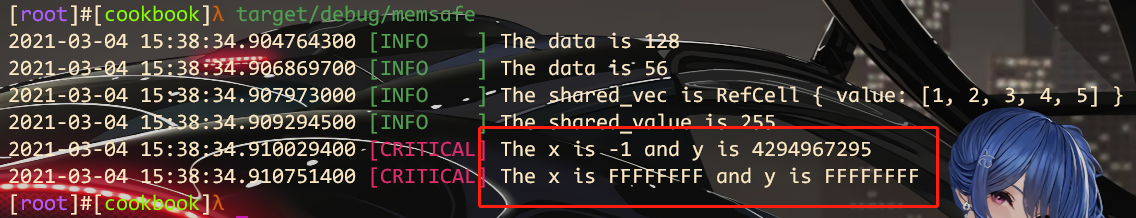
\includegraphics[width=\linewidth]{rust_raw_pointer.png}
  \caption{具有潜在错误的裸指针示例}
  \label{fig:rust_raw_pointer}
\end{figure}
x变成和y一样的值的原因在于:对指向y的指针类型做了转换,让它以为自己指向的是i64
类型,恰巧x就在y旁边,y被修改的同时,就顺带把x也修改了。因此,使用unsafe必须特别
小心。

在通常的情况下,虽然可以通过引用+mut的方式,可以阻止大部分的内存不安全问题,但是
由于引用+mut的强限制性,也为带来一些比较麻烦和无奈的问题,比如下面的代码:
\begin{code-block}{rust}
#[derive(Debug)]
struct Tuple {
    first: u8,
    second: u8,
    third: u8,
}
fn main() {
    let mut t = Tuple {
        first: 0,
        second: 1,
        third: 2,
    };
    let pa = &mut t.first;
    let pb = &mut t.second;
    let pc = &mut t.third;
    *pc += 10;
    info!("{:?}", t);
}
\end{code-block}
上述代码是正确无误的,可以正常编译和运行,但是,如果我们将结构体变成数组,问题就
出现了:
\begin{code-block}{rust}
fn main() {
    let mut array_x = [1_i32, 2, 8];
    let pa = &mut array_x[0];
    let pb = &mut array_x[1];
    *pb += 10;
    info!("{:?}", t);
}
\end{code-block}
上述代码在Rust 1.50.0版本之前就会出现错误:
\begin{code-block}{bash}
error: cannot borrow `x[..]` as mutable more than once at a time
\end{code-block}
原因在于,在Rust 1.50.0版本之前的结构体当中,pa,pb和pc指向不同的内存区域;
但是在数据当中,Rust编译器会将[\_]识别为一个整体,而\&[0], \&[1]之间都属于重叠,
将pa和pb判断为存在别名关系,即pa和pb实质上相同,违反了借用规则,因此无法通过编译。
采用引用分割才能进行解决:
\begin{code-block}{bash}
let mut array_x = [1_i32, 2, 3];
// 通过split_at_mut将数组切分成2个一定不会重叠的切片
let (first, rest): (&mut [i32], &mut [i32]) = array_x.split_at_mut(1);
let (second, third): (&mut [i32], &mut [i32]) = rest.split_at_mut(1);
first[0] += 100;
second[0] += 200;
third[0] += 300;
info!("{:?}", array_x);
\end{code-block}

由于Rust的目标是系统级的语言,必然需要具备操作硬件,以及裸设备的能力。而这些能力,
在C/C++的表述当中,通常是采用共用体(Union)实现的。为了与之兼容,Rust当中也引入了
Union数据结构,其主要的使用形式如下:
\begin{code-block}{rust}
#[repr(C)]
pub union U {
    pub i: u32,
    pub f: f32,
}

#[repr(C)]
pub struct Value {
    pub tag: u8,
    pub value: U,
}
\end{code-block}
其中,\#[repr(C)]必须使用,因为union的使用场景本身就是为了和C/C++进行对接,表示
该联合体使用和C/C++一样的内存布局。由于在字段当中使用了union,因此,结构体Value
也必须添加repr属性,否则会出现未定义的错误。而在使用的时候,则更加需要注意,只要
是涉及到读取联合体的字段,则必须使用unsafe:
\begin{code-block}{rust}
// 禁用illegal_floating_point_literal_pattern警告
#[allow(illegal_floating_point_literal_pattern)]
pub fn is_zero(v: &Value) -> bool {
    unsafe {
        match &v {
            Value {
                tag: Tag::I,
                value: U { i: 0 },
            } => true,
            Value {
                tag: Tag::F,
                // 会出现#[warn(illegal_floating_point_literal_pattern)]警告
                // 目前rust正在修复该问题
                value: U { f: 0.0 },
            } => true,
            _ => false,
        }
    }
}
\end{code-block}

Rust所有的unsafe实际都来源于性能和C的结合(比如写linux内核模块),因此原生指针
在unsafe当中最为常用。其主要的用途如下:
\begin{itemize}
  \item 在必要的时候跳过Rust安全检查:有的情况下,程序逻辑不会有任何内存安全的问题,原生指针可以跳过安全检查,提升性能
  \item 与C语言进行交互,必须使用原生指针
\end{itemize}

空指针在C语言当中非常常见,Rust当中也可以创建原生的空指针,也可以利用原生指针修改
数据:
\begin{code-block}{rust}
// 创建一个指向unsigned char的原生null指针
let pointer: *const u8 = std::ptr::null();
// 判断指针是否为空
assert!(pointer.is_null());

let mut s = [1, 2, 3];
// 创建一个可变的指针,该指针指向一个unsigned int的数组
let pointer: *mut u32 = s.as_mut_ptr();
assert!(!pointer.is_null());

unsafe {
    // 访问s[1]
    info!("The offset 1 is {}", *pointer.offset(1));
    // 访问s[2]
    info!("The offset 2 is {}", *pointer.offset(2));
    // 修改s[2]
    *pointer.offset(2) = 4;
    info!("The offset 2 is {}", *pointer.offset(2));
    // 将s[2]先转换成u8,然后再转换成char
    info!("The offset 2 is {}", *pointer.offset(2) as u8 as char);
}

info!("The final result of s is {:?}", s);
\end{code-block}

\section{杂项与技巧}

\subsection{预处理脚本与依赖关系}
在Rust当中,有的时候需要传递环境变量(编译期间)给源代码,生成特定的内容,此时
如果是直接在源代码当中进行环境变量的获取,则有可能获取到的是错误的信息。这种情况下
可以使用\colorblock{build.rs}脚本进行预处理。包含了该脚本的Rust工程结构大致如下:
\begin{figure}[H]
  \centering
  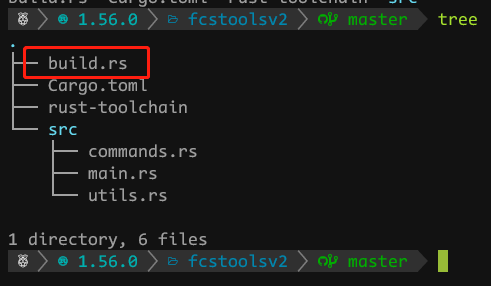
\includegraphics[width=\linewidth]{rust_build_rs.png}
  \caption{包含build.rs的工程结构}
  \label{fig:rust_build_rs}
\end{figure}

一个具体的build.rs实例如下:
\begin{code-block}{rust}
use std::process::Command;

fn main() {
    let output = Command::new("git")
        .args(&["rev-parse", "HEAD"])
        .output()
        .unwrap();
    let git_hash = String::from_utf8(output.stdout).unwrap();

    let __status__ = Command::new("git")
        .args(&["status", "--short"])
        .output()
        .unwrap();

    if "" != String::from_utf8(__status__.stdout).unwrap() {
        println!(
            "cargo:rustc-env=GIT_HASH={}-dirty",
            git_hash.trim_end_matches('\n')
        );
    } else {
        println!("cargo:rustc-env=GIT_HASH={}", git_hash);
    }
}
\end{code-block}

而在真正的源代码当中,使用则类似如下:
\begin{code-block}{rust}
...
let msg = format!(
    "For maintenance the AI Edge Platform, \nbuilt githash {}",
    env!("GIT_HASH"),
);
...
\end{code-block}

默认情况下,build.rs只会使用Rust标准库当中的所有函数和方法,即使是工程的Cargo.toml
文件的\codeinline{toml}{[dependencies]}引入了需要的依赖关系,build.rs仍然无法识别
相关的依赖包。如果需要在build.rs当中使用第三方的开发库,则需要修改工程的Cargo.toml
文件,添加如下的内容:
\begin{code-block}{rust}
# 表示给build.rs使用的依赖库
[build-dependencies]
chrono = "0.4.19"
\end{code-block}

注意,\codeinline{toml}{[dependencies]}和\codeinline{rust}{[build-dependencies]}当中
的依赖库是相互独立不影响的。如果build.rs当中的执行结果和预期的不一致,则可以直接
使用\codeinline{rust}{println!}进行输出打印,但是,这些信息不会在控制台上显示出来,
而是在\codeinline{bash}{target/xxx/build/yyy/output}当中,可以直接进行查看。

\section{常见错误处理方法}
由于很多代码都是第三方的,而Rust本身也在不断的发展,有可能出现版本不兼容或者特性
不兼容的情况,此时,则需要进行相关的修改。比如下面的一种错误:
\begin{figure}[H]
  \centering
  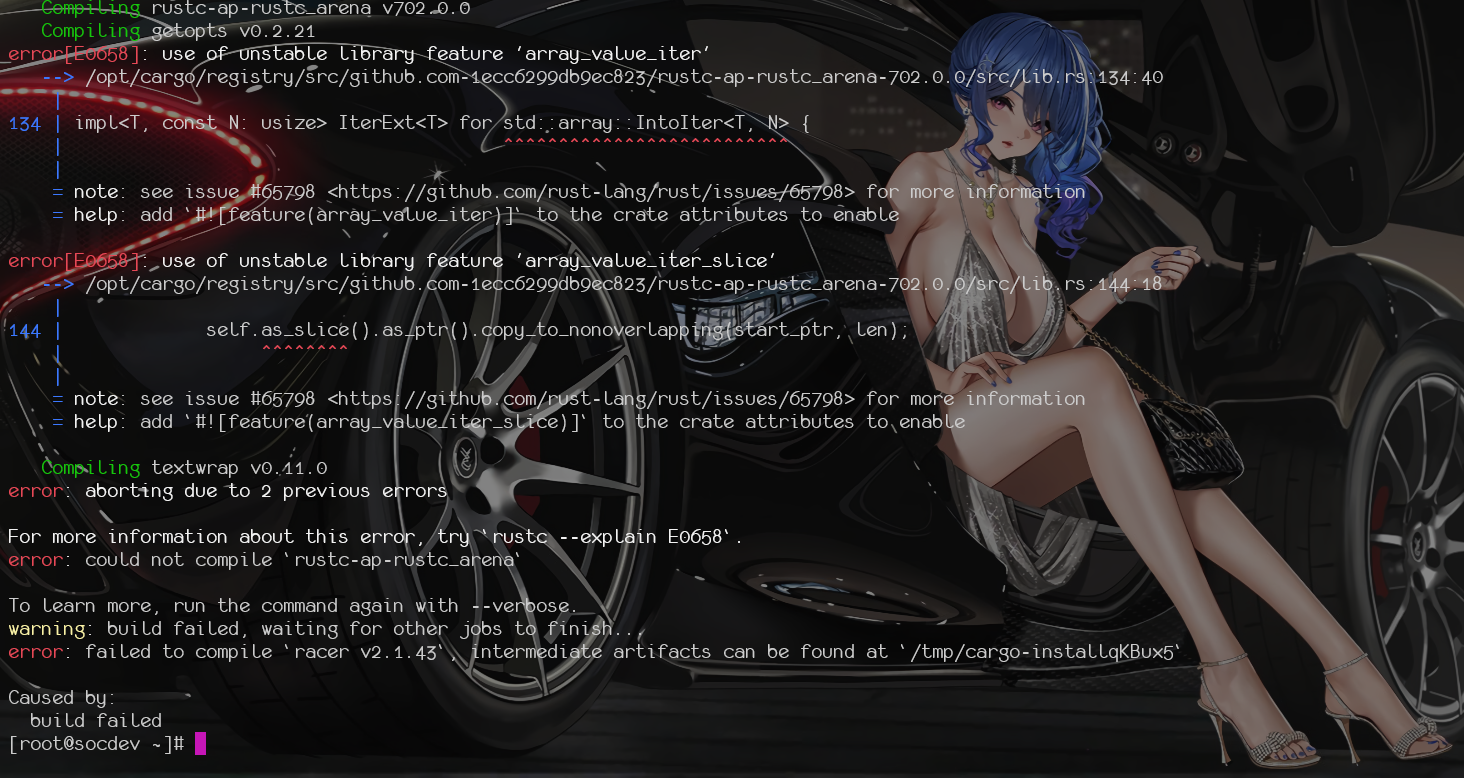
\includegraphics[width=\linewidth]{rust_feature_error.png}
  \caption{缺少特性支持编译失败}
  \label{fig:rust_feature_error}
\end{figure}
遇到这种错误,则需要直接修改对应的类库的源代码。以上述错误为例,编译的help表示
需要添加代码\codeinline{bash}{add `#![feature(array_value_iter_slice)]` to the crate attributes to enable},
则我们应当在对应的crate的lib.rs的头部当中,添加内容如下:
\begin{figure}[H]
  \centering
  
\includegraphics[width=\linewidth]{rust_feature_add.png}
  \caption{增加特性支持}
  \label{fig:rust_feature_add}
\end{figure}

\section{死灵书与实践}

\subsection{随机数实践}
Rust的随机数模块并不包含在标准库当中,需要使用rand这个crate,其基本的使用如下:
\begin{code-block}{rust}
use rand::distributions::{Distribution, Uniform};
use rand::seq::IteratorRandom;
use rand::Rng;
fn main() {
    let mut rng = rand::thread_rng();
    // 生成随机数
    info!("The float64 rand number is {}", rng.gen::<f64>());
    info!("The u32 rand number is {}", rng.gen::<u32>());
    info!("The i32 rand number is {}", rng.gen::<i32>());
    info!("The u8 rand number is {}", rng.gen::<u8>());
    // 从指定区间生成随机数
    info!("The range rand number is {}", rng.gen_range(0..100));
    info!(
        "The range rand float number is {}",
        rng.gen_range(10.0..50.0)
    );
    // 从[0, 5]生成随机数
    info!("The range rand number is {}", rng.gen_range(0..=5));
    // 定义[1, 7)的均匀分布
    let die = Uniform::from(1..7);
    // 从该分布当中生成采样
    let throw = die.sample(&mut rng);
    info!("The sample of uniform is {:>width$}", throw, width = 5);
    // 生成多个随机数
    let tuple: (u8, u8, u8) = rng.gen();
    info!("The tuple of random is {:?}", tuple);
    // 生成随机数组
    let array: [u8; 6] = rng.gen();
    info!("The array of random is {:?}", array);
    let mut exsit_array: [u8; 5] = [1, 2, 34, 5, 6];
    // 使用随机数填充已存在的数组
    rng.fill(&mut exsit_array);
    info!("The array of random is {:?}", exsit_array);
    // 从均匀分布当中随机采样3个数据
    // 得到的结果可能出现重复的情况
    let samples: Vec<u8> = (&mut rng).sample_iter(die).take(3).collect();
    info!("The samples of sample range 1..7 is {:?}", samples);
    let v = vec![1, 2, 3, 4, 5];
    // 从vec当中采样4个数据,得到的结果不会重复
    let sample = v.iter().choose_multiple(&mut rng, 4);
    info!("The samples of sample range 1..5 is {:?}", sample);
    let sample: Vec<u8> = (1..=10).choose_multiple(&mut rng, 4);
    info!("The samples of sample range 1..10 is {:?}", sample);
}
\end{code-block}

Rust的rand crate不仅可以生成随机数,也可以生成自定义的随机数据,比如:
\begin{code-block}{rust}
use rand::distributions::{Distribution, Standard, Uniform};
use rand::seq::IteratorRandom;
use rand::Rng;
struct Point {
    x: u8,
    y: u8,
}
impl fmt::Display for Point {
    fn fmt(&self, f: &mut fmt::Formatter) -> fmt::Result {
        write!(f, "x: {}, y: {}", self.x, self.y)
    }
}
// 在 Point 类型之上,对Standard实现Distribution trait,使得Point可以被gen函数随机生成
impl Distribution<Point> for Standard {
    // 默认的实现方法
    fn sample<R: Rng + ?Sized>(&self, rng: &mut R) -> Point {
        let (rand_x, rand_y) = rng.gen();
        Point {
            x: rand_x,
            y: rand_y,
        }
    }
}
fn main() {
    let mut rng = rand::thread_rng();
    let rand_point = rng.gen::<Point>();
    info!("The rand_point is {}", rand_point);
}
\end{code-block}

同样的,可以生成随机的字符串:
\begin{code-block}{rust}
use rand::distributions::{Alphanumeric, Distribution, Standard, Uniform};
use rand::seq::IteratorRandom;
use rand::Rng;
fn main() {
    let mut rng = rand::thread_rng();
    let rand_string: String = (&mut rng)
        // 从a-z,A-Z以及0-9当中进行选择
        .sample_iter(&Alphanumeric)
        // 获取其中的10个元素
        .take(10)
        // 默认的结果是char类型,需要继续转换成String
        .map(char::from)
        .collect();
    info!("The rand_string is {}", rand_string);
}
\end{code-block}

如果默认的字符集不满足要求,还可以自定义字符集,比如下面的示例:
\begin{code-block}{rust}
use rand::distributions::{Alphanumeric, Distribution, Standard, Uniform};
use rand::seq::IteratorRandom;
use rand::Rng;
const CHARSET: &[u8] = b"ABCDEFGHIJKLMNOPQRSTUVWXYZ\
    abcdefghijklmnopqrstuvwxyz\
    0123456789)(*&^%$#@!~";
const PASSWORD_LEN: usize = 10;
fn main() {
    let mut rng = rand::thread_rng();
    let password: String = (0..PASSWORD_LEN)
        .map(|_| {
            let idx = rng.gen_range(0..CHARSET.len());
            CHARSET[idx] as char
        })
        .collect();
    info!("The password is {}", password);
    // 也可以更换成之前的采样函数,看起来更为精炼
    let passwd: String = CHARSET
        .choose_multiple(&mut rng, 10)
        .map(|r| *r as char)
        .collect();
    info!("The password is {}", passwd);
}
\end{code-block}

同样的,针对自定义的数据类型,同样可以采用采样方法,进行随机数据的提取:
\begin{code-block}{rust}
use rand::distributions::{Alphanumeric, Distribution, Standard, Uniform};
use rand::seq::IteratorRandom;
use rand::Rng;
#[derive(Debug)]
struct Person {
    name: String,
    age: u8,
}
fn main() {
    let mut rng = rand::thread_rng();
    let persons = vec![
        Person {
            name: "lucifer".to_string(),
            age: 18,
        },
        Person {
            name: "titans".to_string(),
            age: 19,
        },
        Person {
            name: "garuda".to_string(),
            age: 36,
        },
    ];
    // 从person的vec当中,随机抽取2个元素
    let rand_person: Vec<_> = persons.choose_multiple(&mut rng, 2).collect();
    info!("The rand person is {:?}", rand_person);
}
\end{code-block}

\subsection{类型再论}
Rust的类型比较多,char,字符串,整数,浮点数等等。这些基础类型和其他语言比较类似,
但是也包含了自己的特点:比如,char类型占据4个字节,可以存放任何一个unicode字符;
对于ASCII字符,只需要一个字节即可,而一个字节的数据,则可以放在u8类型的数据当中,
因此,对于ASCII类型的字符串/字符数组,可以使用u8类型(即单字节)的数组进行存放,
这样,占用的资源空间会比char的数组小:
\begin{code-block}{rust}
fn main() {
    // 字符串前面的b,表示将对应的字面量存放在u8类型当中
    let s: &[u8] = b"hello";
    info!("{:?}", s);
}
\end{code-block}
同时,Rust支持的整数类型比较广泛,包括8bit,16bit,32bit,64bit,最大可以支持到
128bit;而特殊的isize和usize,则是和平台相关。如果平台是32位的,则isize和usize为
32位,如果是64位,则其数据宽度为64位。

整个Rust的类型当中,只有空类型占据的空间是最小的,都是0。Rust的空类型包括单元类型
(unit,即空元组)以及空结构体:
\begin{code-block}{rust}
// empty是空元组类型
let empty : () = ();
// 空结构体
struct Empty();
\end{code-block}
为了查看类型所占用的空间,可以使用size\_of函数进行查看:
\begin{code-block}{rust}
use std::mem;
struct Empty();
fn main() {
    info!("The Empty struct size is {}", mem::size_of::<Empty>());
    // 查看空元组所占据的内存大小
    info!("The none tuple size is {}", mem::size_of::<()>());
}
\end{code-block}

在Rust当中,浮点类型是非常特殊的数据类型。浮点类型当中,存在一个特殊的值:NaN,
即非法的浮点数值,因为该数据的存在,浮点数不具备全序关系(total order)。所谓的
全序,偏序,Rust当中的定义如下:对于集合X当中的元素a,b,c
\begin{itemize}
  \item 如果a<b,则!(a>b)一定成立;反之,如果a>b,则!(a<b)一定成立,即反对称性
  \item 如果a<b,b<c,则a<c,即传递性
  \item 对于X当中的所有元素,都存在a<b,或者a>b,或者a==b,三者必居其一,即完全性
\end{itemize}
如果X集合只满足前面2条,则称之为偏序;具备上述所有特征,则为全序。由于浮点数的NaN
不满足上述第3条规则,因此,Rust的浮点数属于偏序,而非全序,这回导致一个问题:浮点
数无法排序——非NaN的数值无法与NaN进行比较:
\begin{code-block}{rust}
let nan = std::f32::NAN;
let x = 0.4f32;
// 下列结果全部为false
info!("{}", nan > x);
info!("{}", nan < x);
info!("{}", nan == x);
\end{code-block}
为此,Rust设计了2个Trait表示全序与偏序:\codeinline{rust}{std::cmp::Ord}(全序)以及
\codeinline{rust}{std::cmd::PartialOrd}(偏序)。
PartialOrd这个Trait的partial\_cmp方法返回的是Option<Ordering>,而Ord返回的却是
Ordering。Rust的f32和f64都只实现了PartialOrd,因此,浮点类型无法进行排序,也同样无法
求取最值,如下列代码,则是无法运行的:
\begin{code-block}{rust}
let f_vec = vec![1f32, 2.0, 4.0, 0.0, -1.2];
let bigest_f = f_vec.iter().max();
\end{code-block}
对上诉代码进行编译,会直接提示如下类似的错误:
\begin{figure}[H]
  \centering
  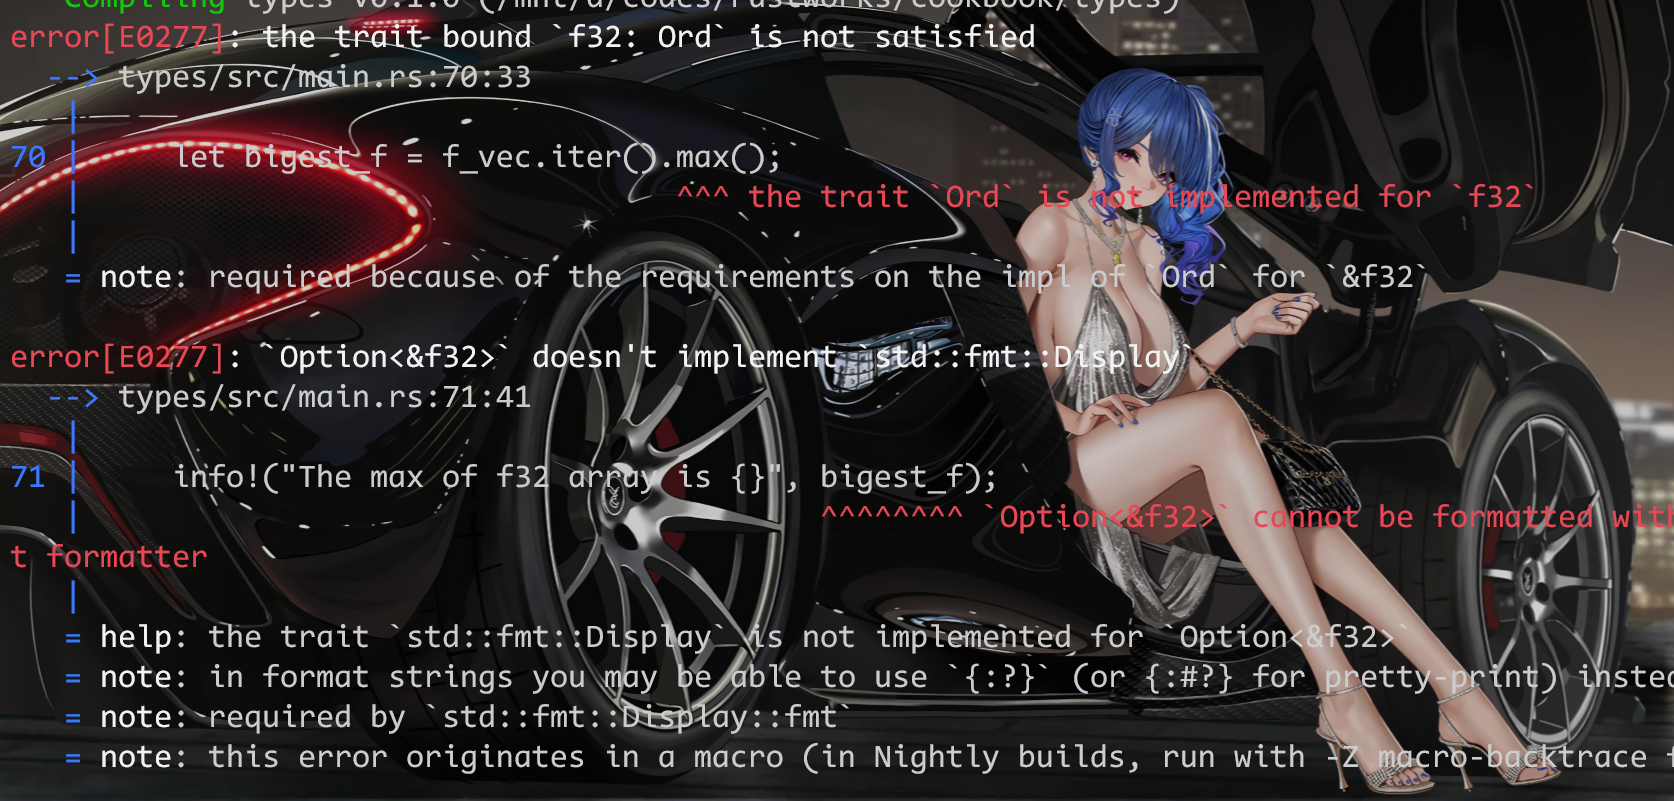
\includegraphics[scale=0.2]{rust_float_cmp_error.png}
  \caption{浮点数的最值错误求解}
  \label{fig:rust_float_cmp_error}
\end{figure}
浮点数的排序只能通过partial\_cmp(比较相等关系)进行变换处理,如下方代码:
\label{float_sort}
\begin{code-block}{rust}
let mut f_vec = vec![1f32, 2.0, 4.0, 0.0, -1.2];
// 升序排列
f_vec.sort_by(|first, second| first.partial_cmp(second).unwrap());
// 获取排序后的最后一位
let max = f_vec.last().unwrap();
// 或者如下进行
// let max = f_vec.as_slice().last().unwrap();
// 降序排列
f_vec.sort_by(|first, second| second.partial_cmp(first).unwrap());
\end{code-block}

作为常用数据类型之一,Rust的数组也存在自己的特点,比如同类型的数组之间可以相互赋值:
\begin{code-block}{rust}
let mut array: [u32; 4] = [1, 23, 4, 5];
let array_copy: [u32; 4] = [5, 6, 7, 8];
array = array_copy;
\end{code-block}
支持数组之间的直接比较,只是数组当中的元素本身就可以进行比较才行:
\begin{code-block}{rust}
let array: [u32; 4] = [1, 23, 4, 5];
let array_copy: [u32; 4] = [5, 6, 7, 8];
info!("{:?}", array < array_copy);
\end{code-block}

Rust当中的函数也可以称之为类型的一种,并且,每个函数都有自己单独的类型,函数的类型
是fn。但是,函数的参数列表会影响fn类型的判断和表达,比如下面的例子:
\begin{code-block}{rust}
fn add_tuple(t: (u32, u32)) -> u32 {
    t.0 + t.1
}
fn add_two((x, y): (u32, u32)) -> u32 {
    x + y
}
fn add_normal(x: u32, y: u32) -> u32 {
    x + y
}
\end{code-block}
实际上,add\_tuple和add\_two这2个函数被fn类型识别成为具有相同签名的类型,因此,
在理论上,我们可以使用同一个变量,接收这2个函数的指针:
\begin{code-block}{rust}
fn main() {
    let mut func = add_tuple;
    func = add_two;
    ...
}
\end{code-block}
但是,上述代码却是错误的:虽然签名相同,但是,类型不同:
\begin{figure}[H]
  \centering
  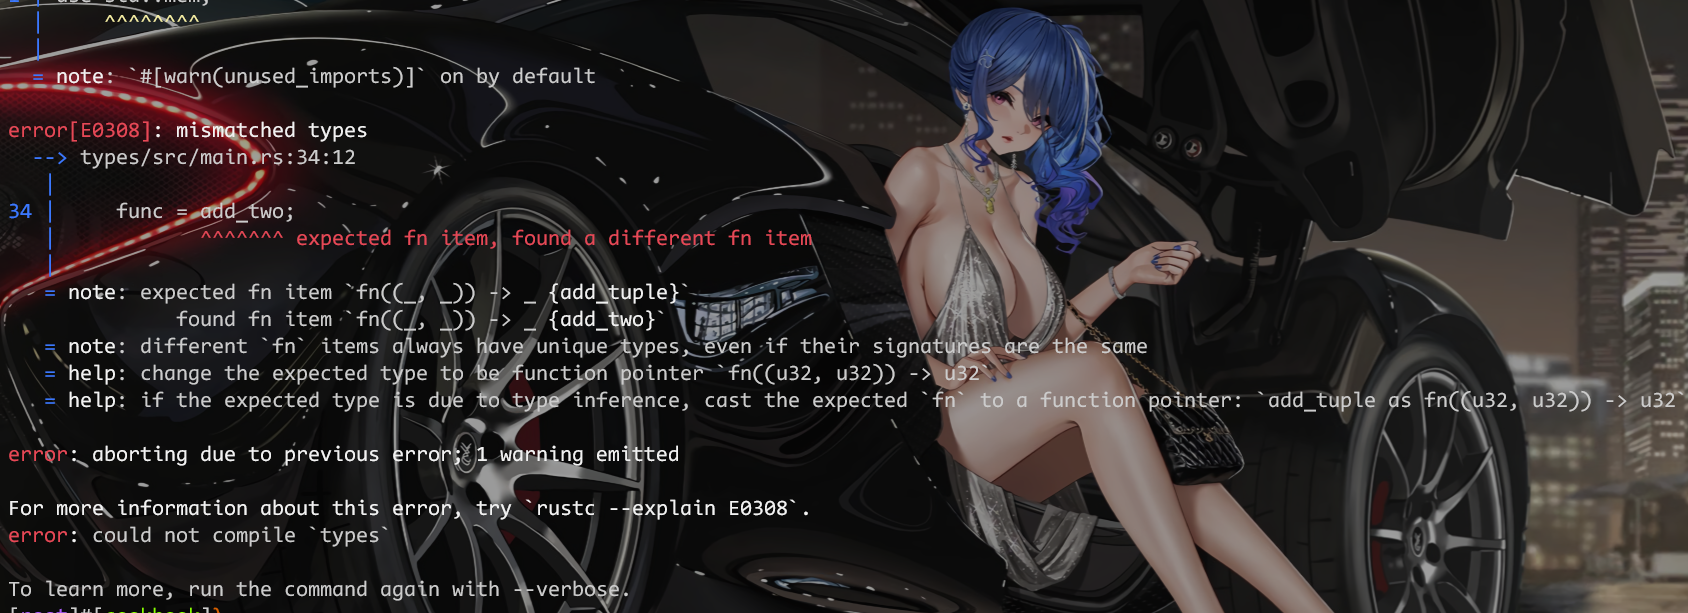
\includegraphics[width=\linewidth]{rust_func_type.png}
  \caption{相同签名的不同函数类型}
  \label{fig:rust_func_type}
\end{figure}
解决方法,则是将其转换成通用的fn类型:
\begin{code-block}{rust}
fn main() {
    // 显示指定func的类型
    let mut func: fn((u32, u32)) -> u32 = add_tuple;
    // 使用as进行类型的转换
    // let mut func = add_tuple as fn((u32, u32)) -> u32;
    func = add_two;
    ...
}
\end{code-block}
但是,需要注意,add\_normal的功能看上去和前面两个函数的功能相同,但是,他们的
函数签名完全不同,因此,不能将其转换成func。

函数是Rust的头等公民,可以在函数/方法当中定义函数,也可以在函数/方法当中定义结构
体,甚至于定义结构体的方法和实现,以及静态变量,常量等:
\begin{code-block}{rust}
fn func_as_first(x: u32, y: u32) -> (u32, u32) {
    struct Point {
        x: u32,
        y: u32,
    };
    impl Point {
        fn area(&self) -> u32 {
            self.x * self.y
        }
        fn cycle(&self) -> u32 {
            self.x + self.y
        }
    };
    let p = Point { x: x, y: y };
    (p.area(), p.cycle())
}
\end{code-block}

常规的函数类型,都会存在返回值,这些返回值要么是特定的类型,要么就是(),即类似
C/C++的返回void。如果需要什么都不返回,则可以使用!,这种函数称之为发散函数,比如
在处理panic时,有时就需要使用发散函数:
\begin{code-block}{rust}
fn diverges() -> ! {
    panic!("This function never returns!");
}
\end{code-block}
Panic操作会直接导致软件栈展开,因此,后续的操作都不会执行,其返回的就是一个!。
发散函数的最大特点,就是可以被转换成任意一个类型,虽然执行的时候最终还是会崩溃,
如下:
\begin{code-block}{rust}
let x : i32 = diverges();
let y : String = diverges();
\end{code-block}
但是,发散函数最大的作用,在于解决编译器的类型检查:
\begin{code-block}{rust}
let p = if x {
    panic!("error");
} else {
    100
};
\end{code-block}
对于let-if而言,if-else的每个分支都必须是相同的数据类型,通过发散函数的任意类型
转换特性即!与任何类型兼容,所以上述代码才能编译通过。

所有的Rust变量,函数都是类型的一种,都可以通过一定的手段和方式,获得类型的具体信息。
常见的方式有两种,一种是使用错误信息进行推断,一种则是使用标准库函数进行获得。

通过构造一个特殊的函数,然后调用该函数,则可以获得相关的类型信息:
\begin{code-block}{rust}
// 接收一个unit参数
fn type_id(_: ()) {}

fn main() {
    let ref i = 5;
    type_id(i);
}
\end{code-block}

而另外的方式,则是使用标准库函数,不过,这个标准库函数在Rust的默认stable分支当中
是不可用的,需要在nightly分支当中进行编译使用,并且,还需要启用一些特性:
\begin{code-block}{rust}
#![feature(core_intrinsics)]
use std;
// 使用泛型参数进行不同类型的数据接收
fn print_type<T>(_arg: &T) {
    println!(
        "The type name of arg is {}",
        std::intrinsics::type_name::<T>()
    );
}
fn main() {
    let ref x = 5;
    print_type(&x);
}
\end{code-block}
编译上述代码时,则需要对编译指令进行部分的调整:
\codeinline{bash}{cargo +nightly build},
然后即可实现对参数类型的打印输出。

在Rust当中,与Python不同,函数/方法并不存在默认参数,但是,结构体当中的字段,却可以
有默认值,只是,这个默认值的实现,必须和Default Trait相结合,如下:
\begin{code-block}{rust}
struct ColoredString {
    input: String,
    fg_color: String,
    bg_color: String,
}
impl Default for ColoredString {
    fn default() -> Self {
        ColoredString {
            input: String::default(),
            fg_color: String::default(),
            bg_color: String::default(),
        }
    }
}
fn main() {
    let color = ColoredString::default();
}
\end{code-block}
从上述代码当中可以看出,实际上,并不是Rust的结构体字段赋予了初始值,而是通过一个
名为default的方法,构造一个我们认为应该具有默认值的结构体。在Rust当中,常用的基本
数据类型都实现了Default Trait,可以直接使用对应的default方法。

\subsection{Trait类型与泛型再论}
关于类型,Trait也是比较重要的一个话题。在之前的示例当中,Trait全部是在具体的类型
上实现的,但是,Trait本身也可以在智能指针(Box)上实现,比如:
\begin{code-block}{rust}
trait Shape {
    fn area(self: Box<Self>) -> f64;
}
struct Circle {
    radius: f64,
}
impl Shape for Circle {
    fn area(self: Box<Self>) -> f64 {
        PI * self.radius * self.radius
    }
}
fn main() {
    let c = Box::new(Circle { radius: 4f64 });
    info!("{}", c.area());
    // 由于trait实现是在智能指针box上,因此,下面的使用是错误的
    // let c = Circle { radius: 4f64 }
    // c.area()
}
\end{code-block}
甚至在Trait上实现Trait,比如下方:
\begin{code-block}{rust}
trait Shape {
    fn area(&self) -> f64;
}
trait Round {
    fn get_radius(&self) -> f64;
}
struct Circle {
    radius: f64,
}
impl Round for Circle {
    fn get_radius(&self) -> f64 {
        self.radius
    }
}
impl Shape for dyn Round {
    fn area(&self) -> f64 {
        let radius = self.get_radius();
        PI * radius * radius
    }
}
\end{code-block}
Shape是一个Trait,Round同样也是一个Trait,Circle实现了Round,Round实现了Shape,
但是,由于Round本身是一个Trait,拥有不确定性,因此,在实现Shape的时候,需要添加
dyn关键字,提示这个Round不是普通的类型,而是一个Trait。上述代码当中,Circle间接
的实现了Shape,但是,Circle的类型无法直接使用Shape的方法,只能通过智能指针的方
式,将Circle转换成Round的类型,再进行使用,如下:
\begin{code-block}{rust}
fn main() {
    let c: Box<dyn Round> = Box::new(Circle { radius: 4f64 });
    info!("{}", c.area());
}
\end{code-block}
如果再把这个例子改得复杂一些,让Circle和Sphere同时实现Round,则我们可以使用Round
指针计算2个不同类型数据的结果:
\begin{code-block}{rust}
trait Shape {
    fn area(&self) -> f64;
}
trait Round {
    fn calc(&self) -> f64;
}
struct Circle {
    radius: f64,
}
impl Round for Circle {
    fn calc(&self) -> f64 {
        PI * self.radius * self.radius
    }
}
struct Sphere {
    radius: f64,
}
impl Round for Sphere {
    fn calc(&self) -> f64 {
        4f64 * PI * self.radius * self.radius
    }
}
impl Shape for dyn Round {
    fn area(&self) -> f64 {
        self.calc()
    }
}
fn main() {
    let circle: Box<dyn Round> = Box::new(Circle { radius: 4f64 });
    info!("The Circle area is {}", circle.area());
    let sphere: Box<dyn Round> = Box::new(Sphere { radius: 4f64 });
    info!("The Sphere area is {}", sphere.area());
}
\end{code-block}

Trait不仅仅用于实现类型,约束类型,还可以用于为其他现有的数据类型添加方法/函数,
比如:
\begin{code-block}{rust}
impl Round for i32 {
    fn calc(&self) -> f64 {
        *self as f64
    }
}
fn main() {
    let i_struct = 4i32;
    i_struct.calc();
}
\end{code-block}
这种类型的函数/方法,则称之为扩展方法/函数。从上述例子当中,我们似乎可以使用Trait
对任意类型进行函数/方法的扩展,但是,这个是存在前提的:
\begin{itemize}
  \item impl和trait的声明/定义在同一个crate当中
  \item 或者,impl的实现需要和类型的声明在同一个crate当中
\end{itemize}
如果不满足上述条件,则容易出现bug和问题,也会违反Rust的规则。

Rust的Trait支持多种特性,自然也支持继承,但是注意,Rust的结构体和enum数据类型并不
存在继承的概念。Trait的继承方式如下:
\begin{code-block}{rust}
trait Base {}
trait Derived : Base {}
\end{code-block}
当一个结构体实现了上述的Derived这个Trait,则必须同样实现Base这个Trait,否则就会
出现语法错误:
\begin{code-block}{rust}
trait Base {}
trait Derived : Base {}
struct T;
impl Derived for T {}
impl Base for T {}
\end{code-block}

Rust的Trait不仅可以包括函数的定义,同样可以直接定义函数:
\begin{code-block}{rust}
trait Page {
    fn set_page(&self) {
        info!("Page Default: 1");
    }
}
trait PerPage {
    fn set_per_page(&self) {
        info!("Per Page Default: 1");
    }
}
struct Paginate {
    page: u32,
}
impl Page for Paginate {}
impl PerPage for Paginate {}
fn main() {
    let page = Paginate { page: 8 };
    page.set_page();
    page.set_per_page();
    page.set_skip_page();
}
\end{code-block}

甚至于,Trait可以直接给结构体提供更多的组合方法:
\begin{code-block}{rust}
trait PaginateMore: Page + PerPage {
    fn set_skip_page(&self) {
        info!("Skip the page");
    }
}
fn main() {
    ...
    page.set_skip_page();
}
\end{code-block}
结构体根本不用自行实现Trait PaginateMore,就可以直接使用该Trait当中的方法。

Trait不仅仅可以用于接口实现,在Rust当中,更重要的则是类型限定,限定某些数据只能
做某些事情。比如下方的代码:
\begin{code-block}{rust}
...
fn static_dispatch<T>(t: &T) where T: Bar {
    ...
}
fn dynamic_dispatch(t : &Bar) {
    ...
}
\end{code-block}
对于实现了Trait Bar的类型来说,上述2个函数,都可以被调用,但是,从语法上,static\_dispatch
由于使用了where,表示参数必须限定在Trait Bar类型,在编译时就能够确定;而dynamic\_dispatch
则从语法上表示,输入的参数必须是Bar的对象,即Trait Object。运行时,Trait Object会根据虚表
指针从虚表当中查出正确的指针,再进行动态调用,属于在运行时确定。

但是并不是每一个Trait都可以当着Trait Object使用,这个和类型大小是否确定有关系。每一个
Trait的隐藏类型参数Self默认限定为?Sized,?Sized trait包括了所有动态大小类型以及所有
可确定大小的类型。Rust当中大部分类型都是默认可确定大小的,即<T:Sized>。当trait对象
在运行期进行动态分发时,也必须确定大小,否则无法分配内存。只有同时满足下列条件的
trait,才可以当作Trait Object使用:
\begin{itemize}
  \item Trait的Self不能被限定为Sized
  \item Trait当中的所有方法都必须是对象安全的
\end{itemize}

而所谓的对象安全,则必须满足如下的条件\colorblock{之一}:
\begin{itemize}
  \item 当Trait的Self被限定为Sized时,方法受Self:Sized约束
  \item Trait的方法签名必须\colorblock{同时满足以下3点}
  \begin{enumerate}
    \item 不包含任何泛型参数(Self)
    \item 第一个参数必须为Self类型或可解引用为Self类型
    \item Self不能出现在除第一个参数之外的其他地方
  \end{enumerate}
  \item Trait当中不能包含关联常量
\end{itemize}

比如下面的代码,就属于标准的对象安全:
\begin{code-block}{rust}
trait Bar {
    fn bax(self, x: u32);
    fn bay(&self);
    fn baz(&mut self);
}
\end{code-block}
Trait Bar不受Sized限制,Trait的方法没有额外的Self类型参数,没有泛型参数,因此是安全的。
相对应的,不安全的Trait如下:
\begin{code-block}{rust}
// 对象不安全
trait Foo {
    fn bad<T>(&self, x:T);
    fn new() -> Self;
}
// 对象安全
trait Foo {
    fn bad<T>(&self, x: T);
    fn new() -> Self
    where
        Self: Sized;
}
\end{code-block}

当然,Sized约束也可以用于Trait定义当中。比如,自行实现一个类似any的Any Trait。
\begin{code-block}{rust}
use std::ops::Fn;
trait CustomAny {
    fn custom_any<F>(&self, f: F) -> bool
    where
        Self: Sized,
        F: Fn(u32) -> bool;
}
impl CustomAny for Vec<u32> {
    fn custom_any<F>(&self, f: F) -> bool
    where
        Self: Sized,
        F: Fn(u32) -> bool,
    {
        for &x in self {
            if f(x) {
                return true;
            }
        }
        false
    }
}
fn main() {
    let v: Vec<u32> = vec![1, 2, 3];
    info!("{}", v.iter().any(|&x| x == 3));
    info!("{}", v.custom_any(|x| x == 3));
}
\end{code-block}

Trait当中不仅可以包含函数和方法,同样可以包含变量和常量,即所谓的关联变量以及关联
常量。关联常量的使用稍微有些特殊,在Trait当中可以定义关联常量,但是,使用的时候,
却是通过Trait的实现对象来使用这些关联常量的:
\begin{code-block}{rust}
trait Colorize {
    // 定义关联常量
    const FG_RED: &'static str = "31";
    const BG_YELLOW: &'static str = "43";
    fn red(self) -> ColoredString;
    fn on_yellow(self) -> ColoredString;
}
impl Colorize for ColoredString {
    fn red(self) -> ColoredString {
        ColoredString {
            // 使用关联常量,如果是Colorize::FG_RED,则会提示错误
            fg_color: String::from(ColoredString::FG_RED),
            ..self
        }
    }
    fn on_yellow(self) -> ColoredString {
        ColoredString {
            bg_color: String::from(ColoredString::BG_YELLOW),
            ..self
        }
    }
}
\end{code-block}

Trait不仅仅可以实现泛型,泛型也不仅限于Trait和<T>,对于函数/方法,也可以使用在
泛型、生命周期以及Trait当中,比如,显式的指定闭包的生命周期:
\begin{code-block}{rust}
// 将函数作为泛型参数
struct Pick<F> {
    data: (u32, u32),
    func: F,
}
impl<F> Pick<F>
where
    // for<>只能用于标记生命周期
    F: for<'f> Fn(&'f (u32, u32)) -> &'f u32,
{
    fn call(&self) -> &u32 {
        (self.func)(&self.data)
    }
}

fn max(data: &(u32, u32)) -> &u32 {
    if data.0 > data.1 {
        return &data.0;
    }
    &data.1
}
fn main() {
    let pick = Pick {
        data: (32, 34),
        func: max,
    };
    info!("{}", pick.call());
}
\end{code-block}

\subsection{常见的设计模式}
建造者模式是Rust当中最常用的设计模式之一,其主旨思想在于将可变和不可变进行分离,
一种基本的示例如下:
\begin{code-block}{rust}
use std::f64::consts;
pub struct Circle {
    radius: f64,
}
pub struct CircleBuilder {
    radius: f64,
}
impl Circle {
    pub fn new() -> CircleBuilder {
        CircleBuilder { radius: 0.0 }
    }
    pub fn area(&self) -> f64 {
        self.radius * self.radius * consts::PI
    }
}
impl CircleBuilder {
    pub fn radius(&mut self, radius: f64) -> &mut CircleBuilder {
        self.radius = radius;
        self
    }
    pub fn build(&self) -> Circle {
        Circle {
            radius: self.radius,
        }
    }
}
\end{code-block}

\subsection{排序}
Rust的整数型数组和向量(Vector)的排序是相同的,可以使用相同的方式进行,即采用
sort以及sort\_unstable进行。其中,sort是稳定排序(即不重新排序相等的元素),
sort\_unstable是不稳定排序,\colorblock{但是通常情况下速度更快},并且不会进行辅助内存的分配。
\begin{code-block}{rust}
let mut v = vec![2, 21, 12, 32, 12, 45, 90];
v.sort_unstable();
info!("The sorted vector is {:?}", v);
let mut array = [2, 23, 12, 12, 98, 100, 21];
array.sort_unstable();
info!("The sorted array is {:?}", array);
\end{code-block}
默认情况下,排序操作使用的是升序,但是可以通过定制,修改排序方式:
\begin{code-block}{rust}
let mut v = vec![2, 21, 12, 32, 12, 45, 90];
// 降序排列,可替换成v.sort_by
v.sort_unstable_by(|a, b| b.cmp(a));
info!("The sorted vector is {:?}", v);
let mut array = [2i32, -23, 12, 12, 98, -100, 21];
// 根据绝对值升序排列,可以根据其他关键字进行排序
array.sort_unstable_by_key(|k| k.abs());
info!("The sorted array is {:?}", array);
// 根据字符顺序排列,带有缓存cache,闭包函数通常只执行一次,比无缓存的快速
let mut xx = [-5i32, 4, 32, -3, 2];
xx.sort_by_cached_key(|k| k.to_string());
// 字符串排序
let mut array = ["lucifer", "titans", "asura", "garuda"];
array.sort_unstable_by_key(|item| item.to_string());
info!("The string array is {:?}", array);
let mut array = [
    "lucifer".to_string(),
    "titans".to_string(),
    "asura".to_string(),
    "garuda".to_string(),
];
// 可以转换成切片
// array[..].sort_unstable_by_key(|item| item.to_string());
// info!("The string array is {:?}", array);
array.sort_unstable_by_key(|item| item.to_string());
info!("The string array is {:?}", array);
\end{code-block}

浮点数的排序和最值操作,参见\colorunderlineref{float_sort}

除了基础数据类型可以进行排序,同样可以针对复合数据类型进行排序。在针对复合数据
类型排序时,需要实现\colorblock{Eq,PartialEq,Ord和PartialOrd}这几个trait:
\begin{code-block}{rust}
#[derive(Eq, PartialEq, Ord, PartialOrd, Debug)]
struct Student {
    name: String,
    age: u8,
}
fn main() {
    let mut stu = [
        Student {
            name: "lucifer".to_string(),
            age: 18,
        },
        Student {
            name: "garuda".to_string(),
            age: 36,
        },
    ];
    // 按照自然序列(name)
    stu.sort();
    info!("The students is {:?}", stu);
    // 根据年龄
    stu.sort_unstable_by(|first, second| first.age.cmp(&second.age));
    info!("The students is {:?}", stu);
}
\end{code-block}

\subsection{压缩与解压}
Rust可以实现文件的压缩与解压,在Linux环境下,通常使用\href{https://github.com/alexcrichton/tar-rs}{tar}(归档)
和\href{https://github.com/rust-lang/flate2-rs}{flate2}(压缩解压),比如Linux下常见的tar.gz文件的处理:
\begin{code-block}{rust}
use flate2::read::GzDecoder;
use flate2::write::GzEncoder;
use flate2::Compression;
use tar::Archive;

let path = "/root/py3.tar.gz";
let targz = match File::open(path) {
    Ok(file) => file,
    Err(error) => {
        crit!("Failed to open the file {}: {}", path, error.to_string());
    }
};
// gz文件的解码器
let tar = GzDecoder::new(targz);
// tar的管理器
let mut archive = Archive::new(tar);
// 将tar.gz解压
match archive.unpack(".") {
    Ok(_) => info!("Sucess to unpack the tar.gz file"),
    Err(error) => {
        crit!("Failed to unpark the tar.gz file: {:?}", error);
    }
}
// 创建tar.gz文件
let targz = match File::create("log.tar.gz") {
    Ok(file) => file,
    Err(error) => {
        crit!(
            "Failed to create the log.tar.gz file : {}",
            error.to_string()
        );
    }
};
// 创建gz文件的编码器,压缩算法使用默认
let encoder = GzEncoder::new(targz, Compression::default());
let mut tarfile = tar::Builder::new(encoder);
// 将文件添加到tar.gz文件当中
match tarfile.append_dir_all("log", "/var/log") {
    Ok(_) => info!("log.tar.gz created sucessful"),
    Err(error) => {
        fs::remove_file("log.tar.gz").unwrap_or_else(|why| {
            error!("Cannot remove the log.tar.gz: {:?}", why.to_string())
        });
        crit!("Failed to park the tar.gz file: {:?}", error);
    }
}
\end{code-block}

当然,归档和压缩也可以单独使用:
\begin{code-block}{rust}
use flate2::read::GzDecoder;
use flate2::write::GzEncoder;
use flate2::Compression;
use tar::Archive;
let tarf = match File::create("log.tar") {
    Ok(file) => file,
    Err(error) => {
        crit!("Failed to create the log.tar file : {}", error.to_string());
    }
};
// 注意和gz文件不一样,只是归档,则不需要创建编码器
let mut tar_file = tar::Builder::new(tarf);
match tar_file.append_dir_all("log", "/var/log") {
    Ok(_) => info!("log.tar created sucessful"),
    Err(error) => {
        fs::remove_file("log.tar")
            .unwrap_or_else(|why| error!("Cannot remove the log.tar: {:?}", why.to_string()));
        crit!("Failed to park the tar.gz file: {:?}", error);
    }
}
let path = "/root/log.tar";
let tarball = match File::open(path) {
    Ok(file) => file,
    Err(error) => {
        crit!("Failed to open the file {}: {}", path, error.to_string());
    }
};
// 同样的,解压tar文件,不需要创建解码器
let mut archive = Archive::new(tarball);
match archive.unpack(".") {
    Ok(_) => info!("Sucess to unpack the tar file"),
    Err(error) => {
        crit!("Failed to unpark the tar file: {:?}", error);
    }
}
\end{code-block}



